% !TeX root = thesis.tex
% !BIB program = biber
% !TEX program = xelatex

%!TEX root = ../thesis.tex

% This information is used in titlepage, colophon, preface and hyperref setup (pdf metainfo), and other options.

%\def\thesistypeabbr{B.Eng.}
%\def\thesistype    {Bachelor of Engineering}
%\def\thesistypeabbr{B.Sc.Eng.}
%\def\thesistype    {Bachelor of Science in Engineering}
%\def\thesistypeabbr{M.Sc.}
%\def\thesistype    {Master of Science in Engineering}
\def\thesistypeabbr{Ph.D.}
\def\thesistype    {Doctor of Philosophy}

\def\thesisdepshort{DTU Compute}
\def\thesisdep     {Department of Applied Mathematics and Computer Science}

\def\thesisauthor  {Jakob Drachmann Havtorn}
\def\thesistitle   {Uncertainty Estimation for Machine Learning Systems}
\def\thesissubtitle{Self-assessment on Medical Conversations}
\def\thesislocation{Copenhagen}
\def\thesisyear    {2023}
\def\thesismonth   {August}
\def\thesisday     {31}

\def\papersize     {b5paper} % Final papersize (b5paper/a4paper), recommended papersize for DTU Compute is b5paper
\def\showtrims     {false}   % Print on larger paper than \papersize and show trim marks (true/false)?
\def\showframe     {false}   % Show frame of writeable area, marginparsep and marginpar (true/false)?

\def\showtodos     {true}    % Show todos (true/false)?
\def\confidential  {false}   % Confidential thesis (true/false)?

\def\skippaperbody {true}    % Skip compiling paper bodies (true/false)?

%!TEX root = ../thesis.tex

% Package that captures and warns against deprecated LaTeX patterns and syntax.
% Included first to capture from document top.
\RequirePackage[l2tabu,orthodox]{nag}

% Paper size switch command (used in \documentclass which is in main file, in order to identify it as such)
\newcommand{\papersizeswitch}[3]{\ifnum\strcmp{\papersize}{#1}=0#2\else#3\fi}
\papersizeswitch{a4paper}{\def\classfontsize{10pt}}{\def\classfontsize{12pt}}


\documentclass[\classfontsize,\papersize,twoside,showtrims,extrafontsizes]{memoir}  % identifies main document in Overleaf

%!TEX root = ../thesis.tex

\RequireXeTeX

\showtrimsoff
\papersizeswitch{b5paper}{
    % Stock and paper layout
    \pagebv
    \setlrmarginsandblock{24mm}{20mm}{*}
    \setulmarginsandblock{30mm}{30mm}{*}
    \setheadfoot{8mm}{10mm}
    \setlength{\headsep}{7mm}
    \setlength{\marginparwidth}{18mm}
    \setlength{\marginparsep}{2mm}
}{
    \papersizeswitch{a4paper}{
        \pageaiv
        \setlength{\trimtop}{0pt}
        \setlength{\trimedge}{\stockwidth}
        \addtolength{\trimedge}{-\paperwidth}
        \settypeblocksize{634pt}{448.13pt}{*}
        \setulmargins{2cm}{*}{*}
        \setlrmargins{*}{*}{*}
        \setmarginnotes{17pt}{51pt}{\onelineskip}
        \setheadfoot{\onelineskip}{2\onelineskip}
        \setheaderspaces{*}{2\onelineskip}{*}
    }{
    }
}
\ifnum\strcmp{\showtrims}{true}=0
    % For printing B5 on A4 with trimmarks
    \showtrimson
    \papersizeswitch{b5paper}{\stockaiv}{\stockaiii}
    \setlength{\trimtop}{\stockheight}
    \addtolength{\trimtop}{-\paperheight}
    \setlength{\trimtop}{0.5\trimtop}
    \setlength{\trimedge}{\stockwidth}
    \addtolength{\trimedge}{-\paperwidth}
    \setlength{\trimedge}{0.5\trimedge}
    
    % bigger todos if trim marks
    \setmarginnotes{10pt}{95pt}{\onelineskip}

    \trimLmarks
    
    % put jobname in left top trim mark
    \renewcommand*{\tmarktl}{%
      \begin{picture}(0,0)
        \unitlength 1mm
        \thinlines
        \put(-2,0){\line(-1,0){18}}
        \put(0,2){\line(0,1){18}}
        \put(3,15){\normalfont\ttfamily\fontsize{8bp}{10bp}\selectfont\jobname\ \
          \today\ \ 
          \printtime\ \ 
          Page \thepage}
      \end{picture}}

    % Remove middle trim marks for cleaner layout
    \renewcommand*{\tmarktm}{}
    \renewcommand*{\tmarkml}{}
    \renewcommand*{\tmarkmr}{}
    \renewcommand*{\tmarkbm}{}
\fi

\checkandfixthelayout                 % Check if errors in paper format!
\sideparmargin{outer}                 % Put sidemargins in outer position

% Large environments
\usepackage{microtype}
\usepackage{mathtools}
\usepackage{listings}                 % Source code printer for LaTeX
\usepackage{tikz}
\usepackage{ragged2e}

% Links
\usepackage[hyphens]{url}             % Allow hyphens in URL's
\usepackage[unicode=false,psdextra]{hyperref}                 % References package

% Graphics and colors
\usepackage{graphicx}                 % Including graphics and using colours
\usepackage{xcolor}                   % Defined more color names
\usepackage{eso-pic}                  % Watermark and other bag
\usepackage{preamble/dtucolors}
\graphicspath{{graphics/}}
\usepackage{caption}
\usepackage[labelformat=simple]{subcaption}
\usepackage[figuresleft]{rotating}
% Enable replacing all sidewaystable environments with regular table environments
\ifthenelse{\equal{\usesidewaystables}{true}}{}{
  \renewenvironment{sidewaystable}{%
      \begin{table}%
  }{%
      \end{table}%
      \ignorespacesafterend%
  }
  \renewenvironment{sidewaystable*}{%
      \begin{table*}%
  }{%
      \end{table*}%
      \ignorespacesafterend%
  }
}


% Language
% \usepackage{polyglossia}    % multilingual typesetting and appropriate hyphenation
% \setdefaultlanguage{english}
\usepackage[english]{babel}
\usepackage{csquotes}       % language sensitive quotation facilities

% Bibliography (references)
% https://tex.stackexchange.com/questions/89842/how-to-print-only-year-no-day-month-with-biblatex            
\usepackage[
  backend=biber,
  natbib=true, 
  style=numeric,
  abbreviate=false,
  dateabbrev=false,
  maxbibnames=14,
  urldate=short,
  backref=true,
  alldates=year
]{biblatex}
\renewcommand*{\bibfont}{\normalfont\footnotesize}  % make bibliography font smaller


\DefineBibliographyStrings{english}{%
  backrefpage = {cited on page},  % originally "cited on page"
  backrefpages = {cited on pages},  % originally "cited on pages"
}

% \newcommand{\printpublication}[1]{\AtNextCite{\defcounter{maxnames}{99}}\fullcite{#1}}  % create new command \printpublication that lists all authors
\preto\fullcite{\AtNextCite{\defcounter{maxnames}{99}}}  % make \fullcite list all authors

\DefineBibliographyExtras{english}{%
  \protected\def\mkbibdatelong#1#2#3{%
    \iffieldundef{#3}
      {}
      {\thefield{#3}%
       \iffieldundef{#2}{}{\nobreakspace}}%
    \iffieldundef{#2}
      {}
      {\mkbibmonth{\thefield{#2}}%
       \iffieldundef{#1}{}{\space}}%
    \iffieldbibstring{#1}{\bibstring{\thefield{#1}}}{\stripzeros{\thefield{#1}}}}%
}


% Highlight own author name
\usepackage{xstring}
\usepackage{etoolbox}
\newboolean{bold}
\newcommand{\makeauthorsbold}[1]{%
  \DeclareNameFormat{author}{%
  \setboolean{bold}{false}%
    \renewcommand{\do}[1]{\expandafter\ifstrequal\expandafter{\namepartfamily}{####1}{\setboolean{bold}{true}}{}}%
    \docsvlist{#1}%
    \ifthenelse{\value{listcount}=1}
    {%
      {\expandafter\ifthenelse{\boolean{bold}}{\mkbibbold{\namepartfamily\addcomma\addspace \namepartgiveni}}{\namepartfamily\addcomma\addspace \namepartgiveni}}%
    }{\ifnumless{\value{listcount}}{\value{liststop}}
      {\expandafter\ifthenelse{\boolean{bold}}{\mkbibbold{\addcomma\addspace \namepartfamily\addcomma\addspace \namepartgiveni}}{\addcomma\addspace \namepartfamily\addcomma\addspace \namepartgiveni}}%
      {\expandafter\ifthenelse{\boolean{bold}}{\mkbibbold{\addcomma\addspace \namepartfamily\addcomma\addspace \namepartgiveni\addcomma\isdot}}{\addcomma\addspace \namepartfamily\addcomma\addspace \namepartgiveni\addcomma\isdot}}%
      }
    \ifthenelse{\value{listcount}<\value{liststop}}
    {\addcomma\space}{}
  }
}
\makeauthorsbold{Havtorn}


% Floating objets, captions and references
% \usepackage{flafter}  % floats is positioned after or where it is defined! 
\setfloatlocations{figure}{tbhp}   % Set floats for all figures
\setfloatlocations{table}{tbhp}    % Set floats for all tables
\setFloatBlockFor{section}         % Typeset floats before each section
\usepackage[noabbrev,nameinlink]{cleveref}  % Clever references. Options: "fig. !1!" --> "!Figure 1!"
\hangcaption
\captionnamefont{\bfseries}
\subcaptionlabelfont{\bfseries}
\newsubfloat{figure}
\newsubfloat{table}
%\letcountercounter{figure}{table}         % Consecutive table and figure numbering
%\letcountercounter{lstlisting}{table}     % Consecutive table and listings numbering
\captiontitlefinal{.}
% strip things from equation references, making them "(1)" instead of "Equation~1"
% from http://tex.stackexchange.com/questions/122174/how-to-strip-eq-from-cleveref
\crefformat{equation}{(#2#1#3)}
\crefrangeformat{equation}{(#3#1#4) to~(#5#2#6)}
\crefmultiformat{equation}{(#2#1#3)}%
{ and~(#2#1#3)}{, (#2#1#3)}{ and~(#2#1#3)}


% Lowercase and uppercase versions of \nameref 
% (from https://tex.stackexchange.com/questions/445404/capitalization-variants-of-nameref)
% - fucnameref: First letter in first word is uppercased
% - ucnameref: All words are uppercased
% - lcnameref: All words are lowercased
\makeatletter
\AtBeginDocument{%
  \newcommand\My@Macro[1]{#1}%
  \newcommand\My@Thirdoffive[5]{\My@Macro{#3}}%
  \renewcommand*\@namerefstar[1]{%
    \HyRef@StarSetRef{#1}\My@Thirdoffive
  }%
  \renewcommand*\T@nameref[1]{%
    \begingroup
    \let\label\@gobble
    \NR@setref{#1}\My@Thirdoffive{#1}%
    \endgroup
  }%
  \DeclareRobustCommand\fucnameref{%
    \@ifstar\fucnameref@star\fucnameref@nostar
  }%
  \newcommand\callemakefirstuc[1]{%
    \MakeLowercase{\emakefirstuc{#1}}%
  }%
  \newcommand\fucnameref@star[1]{%
    \begingroup
    \let\My@Macro=\callemakefirstuc
    \nameref*{#1}%
    \endgroup
  }%
  \newcommand\fucnameref@nostar[1]{%
    \begingroup
    \let\My@Macro=\callemakefirstuc
    \nameref{#1}%
    \endgroup
  }%
  \DeclareRobustCommand\ucnameref{%
    \@ifstar\ucnameref@star\ucnameref@nostar
  }%
  \newcommand\ucnameref@star[1]{%
    \begingroup
    \MFUhyphentrue
    \let\My@Macro=\ecapitalisefmtwords
    \nameref*{#1}%
    \endgroup
  }%
  \newcommand\ucnameref@nostar[1]{%
    \begingroup
    \MFUhyphentrue
    \let\My@Macro=\ecapitalisefmtwords
    \nameref{#1}%
    \endgroup
  }%
  \DeclareRobustCommand\lcnameref{%
    \@ifstar\lcnameref@star\lcnameref@nostar
  }%
  \newcommand\lcnameref@star[1]{%
    \begingroup
    \let\My@Macro=\MakeLowercase
    \nameref*{#1}%
    \endgroup
  }%
  \newcommand\lcnameref@nostar[1]{%
    \begingroup
    \let\My@Macro=\MakeLowercase
    \nameref{#1}%
    \endgroup
  }%
}%
\makeatother


% Table of contents (TOC)
\setcounter{tocdepth}{1}                    % Depth of table of content
\setcounter{secnumdepth}{2}                 % Depth of section numbering
\setcounter{maxsecnumdepth}{3}              % Max depth of section numbering
\renewcommand{\cftdot}{}                    % Remove dots in ToC

\RequirePackage{tocloft}
\PassOptionsToPackage{titles}{tocloft}

% \MakeUppercase breaks hyperlinks
% https://tex.stackexchange.com/questions/605022/how-can-i-use-makeuppercase-in-patchcmd-without-breaking-hyperlinks
% https://groups.google.com/g/comp.text.tex/c/eiLmTiZjKcM
\def\tocnumbersize{\footnotesize}

\renewcommand{\cftpartpresnum}{\scshape}
\renewcommand{\cftpartfont}{\normalsize\color{dtured}\scshape\MakeLowercase}              % \part font in ToC
\renewcommand{\cftpartpagefont}{\tocnumbersize}                                           % \part font in ToC

\renewcommand{\cftchapterpresnum}{\tocnumbersize}%
\renewcommand{\cftchapterfont}{\normalsize\scshape}                                       % \chapter font in ToC
\renewcommand{\cftchapterpagefont}{\tocnumbersize}                                        % \chapter font in ToC

\renewcommand{\cftsectionpresnum}{\tocnumbersize}%
\renewcommand{\cftsectionfont}{\small}                                                    % \section font in ToC
\renewcommand{\cftsectionpagefont}{\tocnumbersize}                                        % \section font in ToC

\renewcommand{\cftsubsectionpresnum}{\tocnumbersize}%
\renewcommand{\cftsubsectionfont}{\small}                                                 % \subsection font in ToC
\renewcommand{\cftsubsectionpagefont}{\tocnumbersize}                                     % \subsection font in ToC

\renewcommand{\cftsubsubsectionpresnum}{\tocnumbersize}%
\renewcommand{\cftsubsubsectionfont}{\small}                                              % \subsubsection font in ToC
\renewcommand{\cftsubsubsectionpagefont}{\tocnumbersize}                                  % \subsubsection font in ToC

\setlength{\cftbeforepartskip}{1em}%
\setlength{\cftbeforechapterskip}{.3em}%
% \setlength{\cftbib}{\cftbeforepartskip}%


% \renewcommand*{\parttitlefont}{\normalfont\large\MakeUppercase}  % font for part title
% \renewcommand*{\partnamefont}{\normalfont\scshape} % font for part name
% \renewcommand*{\partnumfont}{\normalfont\scshape\MakeLowercase}  % font for part number



% Todos
\usepackage{totcount}                                                               % For total counting of counters
\def\todoshowing{}
\ifnum\strcmp{\showtodos}{false}=0
    \def\todoshowing{disable}
\fi
\usepackage[colorinlistoftodos,\todoshowing]{todonotes}                             % Todonotes package for nice todos
\newtotcounter{todocounter}                                                         % Creates counter in todo
\let\oldtodo\todo
\newcommand*{\newtodo}[2][]{\stepcounter{todocounter}\oldtodo[#1]{\thesection~(\thetodocounter)~#2}}
\let\todo\newtodo
\let\oldmissingfigure\missingfigure
\newcommand*{\newmissingfigure}[2][]{\stepcounter{todocounter}\oldmissingfigure[#1]{\thesection~(\thetodocounter)~#2}}
\let\missingfigure\newmissingfigure
\makeatletter
\newcommand*{\mylistoftodos}{% Only show list if there are todos
\if@todonotes@disabled
\else
    \ifnum\totvalue{todocounter}>0
        \markboth{\@todonotes@todolistname}{\@todonotes@todolistname}
        \phantomsection\todototoc
        \listoftodos
    \else
    \fi
\fi
}
\makeatother
\newcommand{\lesstodo}[2][]{\todo[color=green!40,#1]{#2}}
\newcommand{\moretodo}[2][]{\todo[color=red!40,#1]{#2}}


% Chapterstyle
\makeatletter
\makechapterstyle{mychapterstyle}{
    % \chapnamefont
    % \chaptitlefont
    % \printchaptername
    % \printchapternum
    % \printchapternonum
    % \chapternamenum

    \chapterstyle{default}

    \setlength\beforechapskip{0mm}

    \def\format{\normalfont}  % \def\format{\normalfont\sffamily}
    \renewcommand*{\chapnamefont}{\format\fontshape{sc}\selectfont}  % font for chapter text
    % \renewcommand*{\chapnumfont}{\format\fontsize{30}{30}\fontshape{sc}\selectfont}  % font for chapter number
    \renewcommand*{\chapnumfont}{\format\fontsize{13}{13}\fontfamily{eulervm}\selectfont}  % font for chapter number
    \renewcommand*{\chaptitlefont}{\format\fontsize{13}{13}\fontshape{sc}\selectfont}  % font for chapter title

    \renewcommand*{\printchaptername}{\chapnamefont\MakeUppercase{\@chapapp}}  % Uppercase all characters in name
    \patchcommand{\printchaptername}{\begingroup\color{dtured}}{\endgroup}
    \renewcommand*{\chapternamenum}{\space}
    \patchcommand{\printchapternum}{\begingroup\color{dtured}}{\endgroup}
    % \renewcommand*{\printchapternonum}{%
    %     \vphantom{\printchaptername\chapternamenum\chapnumfont 1}
    %     \afterchapternum
    % }

    \setlength\midchapskip{1ex}

    % \renewcommand*{\printchaptertitle}[1]{\raggedleft \chaptitlefont ##1}
    \renewcommand*{\printchaptertitle}[1]{\raggedright \chaptitlefont ##1}
    \renewcommand*{\afterchaptertitle}{\vskip0.5\onelineskip \hrule \vskip1.3\onelineskip}
}
\makeatother
\chapterstyle{mychapterstyle}


% Part style
% \renewcommand*{\thepart}{\arabic{part}}  % redefine the format of the part counter
\renewcommand*{\parttitlefont}{\normalfont\LARGE\scshape}  % font for part title
\renewcommand*{\partnamefont}{\normalfont\large\scshape} % font for part name
\renewcommand*{\partnumfont}{\normalfont\large\scshape}  % font for part number
% Part name and number
\renewcommand*{\printpartname}{{\color{dtured}\partnamefont PART}}  % Command for printing the part name
\renewcommand*{\printpartnum}{{\color{dtured}\partnumfont\thepart}} % Command for printing the part number
% Define skips (used to add horizontal rule)
\renewcommand{\midpartskip}{\par\parbox{0.25\textwidth}{\hrulefill}\par}
\renewcommand{\beforepartskip}{\vspace*{\fill}}
\renewcommand{\afterpartskip}{\vspace*{\fill}}
% For table of contents
\renewcommand*{\cftpartname}{Part}
\renewcommand*{\cftpartpresnum}{\space}
\renewcommand*{\cftpartaftersnum}{.}
\renewcommand*{\cftpartaftersnumb}{\space}


% Header and footer
\def\hffont{\scshape\small}
\makepagestyle{myruled}
\makeheadrule{myruled}{\textwidth}{\normalrulethickness}
\makeevenhead{myruled}{\hffont\thepage}{}{\hffont\leftmark}
\makeoddhead{myruled}{\hffont\rightmark}{}{\hffont\thepage}
\makeevenfoot{myruled}{}{}{}
\makeoddfoot{myruled}{}{}{}
\makepsmarks{myruled}{
    \nouppercaseheads
    \createmark{chapter}{both}{shownumber}{}{\space}
    \createmark{section}{right}{shownumber}{}{\space}
    \createplainmark{toc}{both}{\contentsname}
    \createplainmark{lof}{both}{\listfigurename}
    \createplainmark{lot}{both}{\listtablename}
    \createplainmark{bib}{both}{\bibname}
    \createplainmark{index}{both}{\indexname}
    \createplainmark{glossary}{both}{\glossaryname}
}
\pagestyle{myruled}
\copypagestyle{cleared}{myruled}      % When \cleardoublepage, use myruled instead of empty
\makeevenhead{cleared}{\hffont\thepage}{}{} % Remove leftmark on cleared pages

\makeevenfoot{plain}{}{}{}            % No page number on plain even pages (chapter begin)
\makeoddfoot{plain}{}{}{}             % No page number on plain odd pages (chapter begin)

% \*section, \*paragraph font styles
\setsecheadstyle              {\Large\scshape\raggedright} %{\LARGE\sffamily\raggedright}
\setsubsecheadstyle           {\large\scshape\raggedright} %{\Large\sffamily\raggedright}
\setsubsubsecheadstyle        {\normalsize\scshape\raggedright} %{\large\sffamily\raggedright}
% \setparaheadstyle             {\normalsize\sffamily\itseries\raggedright}
% \setsubparaheadstyle          {\normalsize\sffamily\raggedright}


% Hypersetup
\hypersetup{
    pdfauthor={\thesisauthor{}},
    pdftitle={\thesistitle{}},
    pdfsubject={\thesissubtitle{}},
    pdfdisplaydoctitle,
    bookmarksnumbered=true,
    bookmarksopen,
    breaklinks,
    linktoc=all,
    plainpages=false,
    unicode=true,
    colorlinks=false,
    citebordercolor=dtured,           % color of links to bibliography
    filebordercolor=dtured,           % color of file links
    linkbordercolor=dtured,           % color of internal links (change box color with linkbordercolor)
    urlbordercolor=s13,               % color of external links
    hidelinks,                        % Do not show boxes or colored links.
}
% Hack to make right pdfbookmark link. The normal behavior links just below the chapter title. This hack put the link just above the chapter like any other normal use of \chapter.
% Another solution can be found in http://tex.stackexchange.com/questions/59359/certain-hyperlinks-memoirhyperref-placed-too-low
\makeatletter
\renewcommand{\@memb@bchap}{%
  \ifnobibintoc\else
    \phantomsection
    \addcontentsline{toc}{chapter}{\bibname}%
  \fi
  \chapter*{\bibname}%
  \bibmark
  \prebibhook
}
\let\oldtableofcontents\tableofcontents
\newcommand{\newtableofcontents}{
    \@ifstar{\oldtableofcontents*}{
        \phantomsection\addcontentsline{toc}{chapter}{\contentsname}\oldtableofcontents*}}
\let\tableofcontents\newtableofcontents
\makeatother

% Confidential
\newcommand{\confidentialbox}[1]{
    \put(0,0){\parbox[b][\paperheight]{\paperwidth}{
        \begin{vplace}
            \centering
            \scalebox{1.3}{
                \begin{tikzpicture}
                    \node[very thick,draw=red!#1,color=red!#1,
                          rounded corners=2pt,inner sep=8pt,rotate=-20]
                          {\sffamily \HUGE \MakeUppercase{Confidential}};
                \end{tikzpicture}
            }
        \end{vplace}
    }}
}

% Prefrontmatter
\newcommand{\prefrontmatter}{
    \pagenumbering{alph}
    \ifnum\strcmp{\confidential}{true}=0
        \AddToShipoutPictureBG{\confidentialbox{10}}   % 10% classified box in background on each page
        \AddToShipoutPictureFG*{\confidentialbox{100}} % 100% classified box in foreground on first page
    \fi
}

% DTU frieze
\newcommand{\frieze}[2]{%
    \AddToShipoutPicture*{
        \put(#1,#2){
            \parbox[b][\paperheight]{\paperwidth}{%
                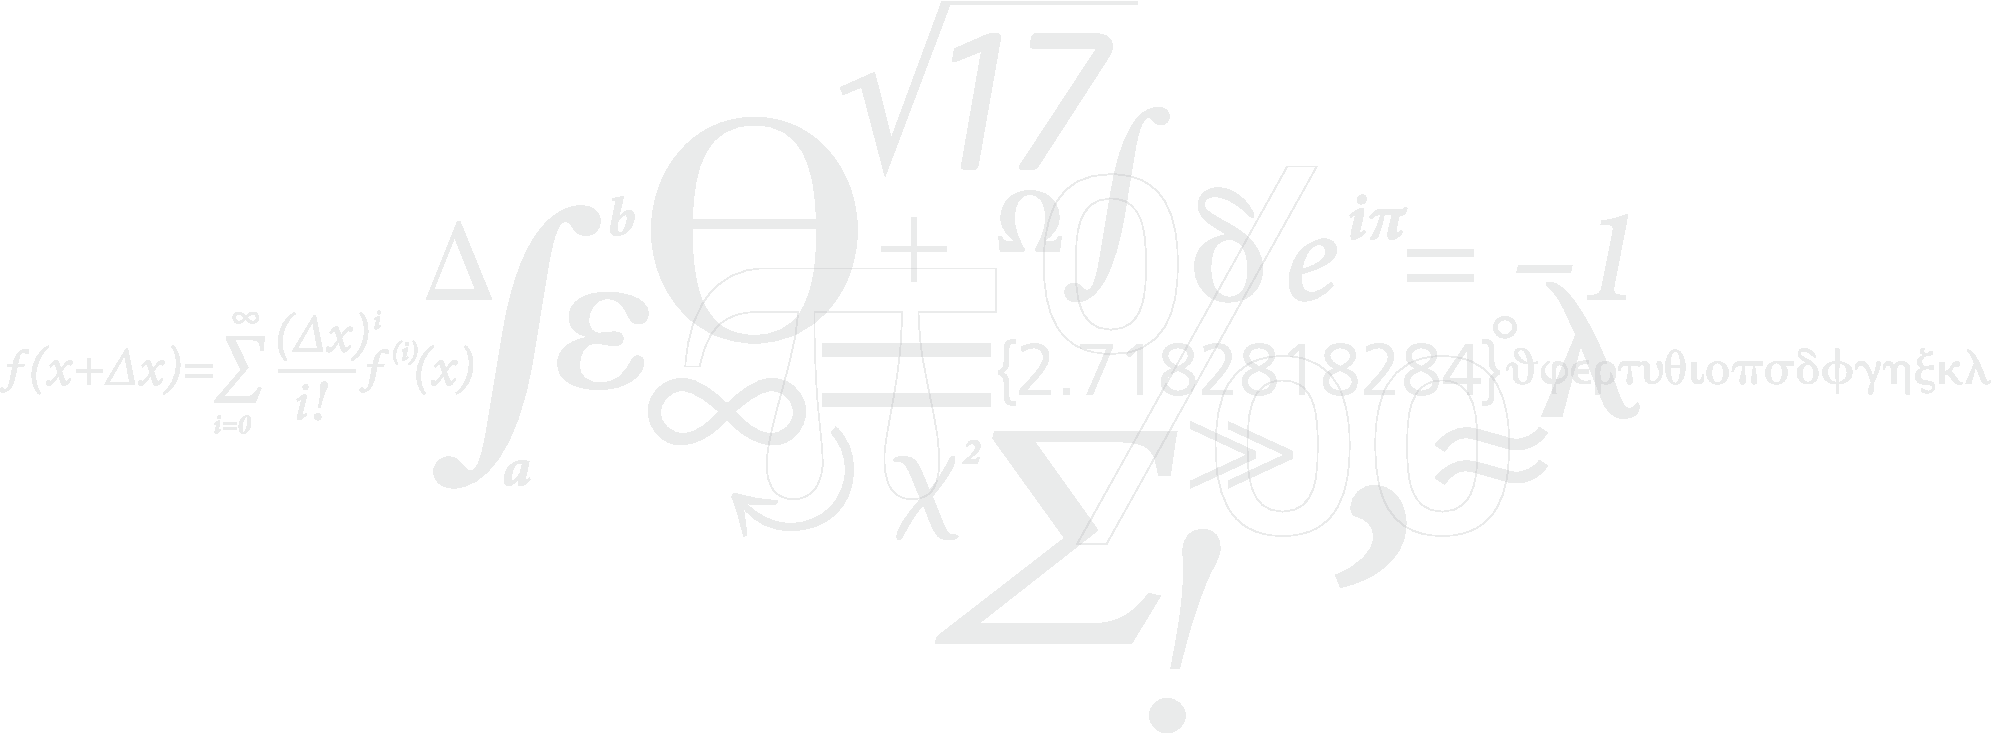
\includegraphics[trim=130mm 0 0 0,width=0.9\textwidth]{DTU-frise-SH-15}
                \vspace*{2.5cm}
            }
        }
    }
}

% This is a double sided book. If there is a last empty page lets use it for some fun e.g. the frieze.
% NB: For a fully functional hack the \clearpage used in \include does some odd things with the sequence numbering. Thefore use \input instead of \include at the end of the book. If bibliography is used at last everything should be ok.
\makeatletter
% Adjust so gatherings is allowd for single sheets too! (hacking functions in memoir.dtx)
\patchcmd{\leavespergathering}{\ifnum\@memcnta<\tw@}{\ifnum\@memcnta<\@ne}{
    \leavespergathering{1}
    % Insert the frieze
    \patchcmd{\@memensuresigpages}{\repeat}{\repeat\frieze{0}{0}}{}{}
}{}
\makeatother


% %% Sharelatex fix for microtype warnings
% \makeatletter
% \def\MT@is@composite#1#2\relax{%
%   \ifx\\#2\\\else
%     \expandafter\def\expandafter\MT@char\expandafter{\csname\expandafter
%                     \string\csname\MT@encoding\endcsname
%                     \MT@detokenize@n{#1}-\MT@detokenize@n{#2}\endcsname}%
%     % 3 lines added:
%     \ifx\UnicodeEncodingName\@undefined\else
%       \expandafter\expandafter\expandafter\MT@is@uni@comp\MT@char\iffontchar\else\fi\relax
%     \fi
%     \expandafter\expandafter\expandafter\MT@is@letter\MT@char\relax\relax
%     \ifnum\MT@char@ < \z@
%       \ifMT@xunicode
%         \edef\MT@char{\MT@exp@two@c\MT@strip@prefix\meaning\MT@char>\relax}%
%           \expandafter\MT@exp@two@c\expandafter\MT@is@charx\expandafter
%             \MT@char\MT@charxstring\relax\relax\relax\relax\relax
%       \fi
%     \fi
%   \fi
% }
% % new:
% \def\MT@is@uni@comp#1\iffontchar#2\else#3\fi\relax{%
%   \ifx\\#2\\\else\edef\MT@char{\iffontchar#2\fi}\fi
% }
% \makeatother\makeatother

%!TEX root = ../thesis.tex

% Text fonts (http://www.macfreek.nl/memory/Fonts_in_LaTeX)
% Install fonts from /usr/local/texlive/<version>/texmf-dist/fonts/opentype/public
\usepackage{fontspec}
\usepackage[T1]{fontenc}
\usepackage{lmodern}
\usepackage{slantsc}
% \RequirePackage{fix-cm}
\usepackage{bold-extra}
\usepackage{upgreek}

% \DeclareFontShape{T1}{texgyrepagella}{b}{sc}{<->ssub*cmr/bx/sc}{}
% \DeclareFontShape{T1}{texgyrepagella}{bx}{sc}{<->ssub*cmr/bx/sc}{}


% % Euler math fonts
% \usepackage[OT1,euler-digits,euler-hat-accent]{eulervm}
% \usepackage[bb=stixtwo]{mathalpha}
% \renewcommand{\mathbf}{\mathbold}  % euler requires \mathbold for bold math

% \usepackage{newtxmath}



% Serif font
% \usepackage{newpxtext}
% \setmainfont{TeX Gyre Pagella}
% \setmainfont{texgyrepagella}



\usepackage{mathpazo} % add possibly `sc` and `osf` options
\usepackage{eulervm}
\renewcommand{\mathbf}{\mathbold}  % euler requires \mathbold for bold math

% % Remove: "Font shape `T1/eulervm/m/n' undefined (Font) using `T1/cmr/m/n' instead."
% \usepackage{substitutefont}
% \substitutefont{TS1}{eulervm}{cmr}

%
% [
%   Extension=.otf,
%   UprightFont=*-regular,
%   ItalicFont=*-italic,
%   BoldFont=*-bold,
%   BoldItalicFont=*-bolditalic,
%   BoldSmallCapsFont=*-boldsmallcaps,
%   Numbers=OldStyle,
% ]

% \setmainfont{QTPalatine}

% \DeclareCharacterInheritance
%    { encoding = {TU,EU1,EU2},
%      family   = {QTPalatine} }
%    { A = {\`A,\'A,\^A,\~A,\"A,\r A},
%      a = {\`a,\'a,\^a,\~a,\"a,\r a},
%      C = {\c C},
%      c = {\c c},
%      D = {\DH},
%      d = {\dj},
%      E = {\`E,\'E,\^E,\"E},
%      e = {\`e,\'e,\^e,\"e},
%      I = {\`I,\'I,\^I,\"I},
%      i = {\`i,\'i,\^i,\"i,\i},
%      L = {\L},
%      l = {\l},
%      N = {\~N},
%      n = {\~n},
%      O = {\O,\`O,\'O,\^O,\~O,\"O},
%      o = {\o,\`o,\'o,\^o,\~o,\"o},
%      S = {\v S},
%      s = {\v s},
%      U = {\`U,\'U,\^U,\"U},
%      u = {\`u,\'u,\^u,\"u},
%      Y = {\'Y,\"Y},
%      y = {\'y,\"y},
%      Z = {\v Z},
%      z = {\v z}
%    }


% % Sans-serif font
% \setsansfont[
%     Ligatures=TeX,
%     Extension=.otf,
%     UprightFont=*-regular,
%     BoldFont=*-bold,
%     ItalicFont=*-italic,
%     BoldItalicFont=*-bolditalic,
%     % SlantedFont=,
%     % BoldSlantedFont=,
%     % SmallCapsFont=
%     Scale=0.8      % Adjustmens when using math in sections
% ]{texgyreadventor}


% Monospaced
% \setmonofont[Scale=MatchLowercase]{Linux Biolinum O}

%\setsansfont[Ligatures=TeX]{Neo Sans Intel}    % Neo Sans Intel – Like DTU font but more symbols
%\setsansfont[
%    Ligatures=TeX,
%    Scale=0.8
%]{NeoSans}           % NeoSans – DTU font (missing `+' symbols and other)
% \setsansfont[Ligatures=TeX]{CMU Sans Serif}    % Computer Modern Unicode font
%\setsansfont[Ligatures=TeX]{Latin Modern Sans} % Latin Modern Sans serif font

% Use this for more convienent sans serif font in math mode.
%\setmathsf{Latin Modern Sans}

%!TEX root = ../thesis.tex

% Content specific packages.

\usepackage{blindtext}
\usepackage{algorithm}
\usepackage{algpseudocode}
\usepackage{multicol}
\usepackage{multirow}
\usepackage{makecell}
\usepackage{booktabs}
\usepackage{enumerate}
\usepackage{enumitem}
% \usepackage{layouts}
\usepackage[showframe=\showframe,xetex]{geometry}
\usepackage{adjustbox}
\usepackage{siunitx}
\usepackage{nomencl}
\usepackage{amsmath}
\usepackage{amssymb}
\usepackage[acronym,toc]{glossaries}
%!TEX root = ../thesis.tex

% \makeglossaries
\makenoidxglossaries


% Glossary

\newglossaryentry{encoder}
{
    name=encoder,
    description={A general term for a function that maps an input to a different representation.}
}

\newglossaryentry{decoder}
{
    name=decoder,
    description={A general term for a function that maps a representation to an output.}
}


% Abbreviations
\newacronym{AI}{AI}{artificial intelligence}

\newacronym{MLP}{MLP}{multilayer perceptron}
\newacronym{FNN}{FNN}{feedforward neural network}
\newacronym{CNN}{CNN}{convolutional neural network}
\newacronym{RNN}{RNN}{recurrent neural network}
\newacronym{LSTM}{LSTM}{long short-term memory}
\newacronym{GRU}{GRU}{gated recurrent unit}
\newacronym{BNN}{BNN}{Bayesian neural network}

\newacronym{ReLU}{ReLU}{rectified linear unit}

\newacronym{SGD}{SGD}{stochastic gradient descent}

\newacronym{SGVB}{SGVB}{stochastic gradient variational Bayes}
\newacronym{VAE}{VAE}{variational autoencoder}
\newacronym{LVM}{LVM}{latent variable model}
\newacronym{KL}{KL}{Kullback-Leibler}

\newacronym{NLL}{NLL}{negative log-likelihood}
\newacronym{MSE}{MSE}{mean squared error}
\newacronym{CCE}{CCE}{categorical cross entropy}
\newacronym{MLE}{MLE}{maximum likelihood estimate}

\newacronym{PCA}{PCA}{principal components analysis}

\newacronym{PDF}{PDF}{probability density function}
\newacronym{PMF}{PMF}{probability mass function}

\newacronym{iid}{iid}{independent and identically distributed}

\newacronym{CPU}{CPU}{central processing unit}
\newacronym{GPU}{GPU}{graphics processing unit}
\newacronym{HPC}{HPC}{high performance computing}



%\usepackage{pgfplots}                 % Plot tools
%\pgfplotsset{compat=1.7}
\usetikzlibrary{
    arrows,
    matrix,
    positioning,
    shapes,
    shapes.multipart,
    topaths,
    bayesnet,
}
% tikzlibrary.code.tex
%
% Copyright 2010-2011 by Laura Dietz
% Copyright 2012 by Jaakko Luttinen
%
% This file may be distributed and/or modified
%
% 1. under the LaTeX Project Public License and/or
% 2. under the GNU General Public License.
%
% See the files LICENSE_LPPL and LICENSE_GPL for more details.

% Load other libraries
\usetikzlibrary{shapes}
\usetikzlibrary{fit}
\usetikzlibrary{chains}
\usetikzlibrary{arrows}

% Latent node
\tikzstyle{latent} = [circle,fill=white,draw=black,inner sep=1pt,
minimum size=20pt, font=\fontsize{10}{10}\selectfont, node distance=1]
% Observed node
\tikzstyle{obs} = [latent,fill=gray!25]
% Constant node
\tikzstyle{const} = [rectangle, inner sep=0pt, node distance=1]
% Factor node
\tikzstyle{factor} = [rectangle, fill=black,minimum size=5pt, inner
sep=0pt, node distance=0.4]
% Deterministic node
\tikzstyle{det} = [latent, diamond]

% Plate node
\tikzstyle{plate} = [draw, rectangle, rounded corners, fit=#1]
% Invisible wrapper node
\tikzstyle{wrap} = [inner sep=0pt, fit=#1]
% Gate
\tikzstyle{gate} = [draw, rectangle, dashed, fit=#1]

% Caption node
\tikzstyle{caption} = [font=\footnotesize, node distance=0] %
\tikzstyle{plate caption} = [caption, node distance=0, inner sep=0pt,
below left=5pt and 0pt of #1.south east] %
\tikzstyle{factor caption} = [caption] %
\tikzstyle{every label} += [caption] %

\tikzset{>={triangle 45}}

%\pgfdeclarelayer{b}
%\pgfdeclarelayer{f}
%\pgfsetlayers{b,main,f}

% \factoredge [options] {inputs} {factors} {outputs}
\renewcommand{\factoredge}[4][]{ %
  % Connect all nodes #2 to all nodes #4 via all factors #3.
  \foreach \f in {#3} { %
    \foreach \x in {#2} { %
      \path (\x) edge[-,#1] (\f) ; %
      %\draw[-,#1] (\x) edge[-] (\f) ; %
    } ;
    \foreach \y in {#4} { %
      \path (\f) edge[->,#1] (\y) ; %
      %\draw[->,#1] (\f) -- (\y) ; %
    } ;
  } ;
}

% \edge [options] {inputs} {outputs}
\renewcommand{\edge}[3][]{ %
  % Connect all nodes #2 to all nodes #3.
  \foreach \x in {#2} { %
    \foreach \y in {#3} { %
      \path (\x) edge [->,#1] (\y) ;%
      %\draw[->,#1] (\x) -- (\y) ;%
    } ;
  } ;
}

% \factor [options] {name} {caption} {inputs} {outputs}
\renewcommand{\factor}[5][]{ %
  % Draw the factor node. Use alias to allow empty names.
  \node[factor, label={[name=#2-caption]#3}, name=#2, #1,
  alias=#2-alias] {} ; %
  % Connect all inputs to outputs via this factor
  \factoredge {#4} {#2-alias} {#5} ; %
}

% \plate [options] {name} {fitlist} {caption}
\renewcommand{\plate}[4][]{ %
  \node[wrap=#3] (#2-wrap) {}; %
  \node[plate caption=#2-wrap] (#2-caption) {#4}; %
  \node[plate=(#2-wrap)(#2-caption), #1] (#2) {}; %
}

% \gate [options] {name} {fitlist} {inputs}
\renewcommand{\gate}[4][]{ %
  \node[gate=#3, name=#2, #1, alias=#2-alias] {}; %
  \foreach \x in {#4} { %
    \draw [-*,thick] (\x) -- (#2-alias); %
  } ;%
}

% \vgate {name} {fitlist-left} {caption-left} {fitlist-right}
% {caption-right} {inputs}
\renewcommand{\vgate}[6]{ %
  % Wrap the left and right parts
  \node[wrap=#2] (#1-left) {}; %
  \node[wrap=#4] (#1-right) {}; %
  % Draw the gate
  \node[gate=(#1-left)(#1-right)] (#1) {}; %
  % Add captions
  \node[caption, below left=of #1.north ] (#1-left-caption)
  {#3}; %
  \node[caption, below right=of #1.north ] (#1-right-caption)
  {#5}; %
  % Draw middle separation
  \draw [-, dashed] (#1.north) -- (#1.south); %
  % Draw inputs
  \foreach \x in {#6} { %
    \draw [-*,thick] (\x) -- (#1); %
  } ;%
}

% \hgate {name} {fitlist-top} {caption-top} {fitlist-bottom}
% {caption-bottom} {inputs}
\renewcommand{\hgate}[6]{ %
  % Wrap the left and right parts
  \node[wrap=#2] (#1-top) {}; %
  \node[wrap=#4] (#1-bottom) {}; %
  % Draw the gate
  \node[gate=(#1-top)(#1-bottom)] (#1) {}; %
  % Add captions
  \node[caption, above right=of #1.west ] (#1-top-caption)
  {#3}; %
  \node[caption, below right=of #1.west ] (#1-bottom-caption)
  {#5}; %
  % Draw middle separation
  \draw [-, dashed] (#1.west) -- (#1.east); %
  % Draw inputs
  \foreach \x in {#6} { %
    \draw [-*,thick] (\x) -- (#1); %
  } ;%
}



\definecolor{customgreen} {RGB}{217	234	212}
\definecolor{customblue}  {RGB}{205	226	242}
\definecolor{custommorered}{RGB}{218 46 42}
\definecolor{customred}{RGB}{255 182 173}%{255 149 150}

\colorlet{observed-color}{customgreen}
\colorlet{latent-color}{customblue}
\colorlet{deterministic-color}{gray!15}
\colorlet{deterministic-skip-color}{custommorered}
\colorlet{shared-function-color}{blue}


% Listings
\lstset{
    basicstyle=\footnotesize\ttfamily,% the size of the fonts that are used for the code
    breakatwhitespace=false,          % sets if automatic breaks should only happen at whitespace
    breaklines=true,                  % sets automatic line breaking
    captionpos=b,                     % sets the caption-position to bottom
    commentstyle=\color{s14a},        % comment style
    deletekeywords={},                % if you want to delete keywords from the given language
    escapeinside={\%*}{*)},           % if you want to add LaTeX within your code
    frame=single,                     % adds a frame around the code
    keywordstyle=\bfseries\ttfamily\color{s09}, % keyword style
    language=Python,                  % the language of the code
    morekeywords={*,...},             % if you want to add more keywords to the set
    numbers=left,                     % where to put the line-numbers; possible values are (none, left, right)
    numbersep=5pt,                    % how far the line-numbers are from the code
    numberstyle=\sffamily\tiny\color{dtugray}, % the style that is used for the line-numbers
    rulecolor=\color{dtugray},        % if not set, the frame-color may be changed on line-breaks within not-black text (e.g. comments (green here))
    showspaces=false,                 % show spaces everywhere adding particular underscores; it overrides 'showstringspaces'
    showstringspaces=false,           % underline spaces within strings only
    showtabs=false,                   % show tabs within strings adding particular underscores
    stepnumber=1,                     % the step between two line-numbers. If it's 1, each line will be numbered
    stringstyle=\color{s07},          % string literal style
    tabsize=2,                        % sets default tabsize to 2 spaces
    title=\lstname,                   % show the filename of files included with \lstinputlisting; also try caption instead of title
}


%!TEX root = ../thesis.tex

% Parenthesis
\providecommand{\pa}[1]{{\left(#1\right)}}
  \renewcommand{\pa}[1]{{\left(#1\right)}}
\providecommand{\bra}[1]{{\left[#1\right]}}
  \renewcommand{\bra}[1]{{\left[#1\right]}}
\providecommand{\cbra}[1]{{\left\{#1\right\}}}
  \renewcommand{\cbra}[1]{{\left\{#1\right\}}}
\providecommand{\vbra}[1]{{\left\langle#1\right\rangle}}
  \renewcommand{\vbra}[1]{{\left\langle#1\right\rangle}}

% Matrices for displayed expressions
\providecommand{\mat}[1]{{\begin{matrix}#1\end{matrix}}}
  \renewcommand{\mat}[1]{{\begin{matrix}#1\end{matrix}}}
\providecommand{\pmat}[1]{{\begin{pmatrix}#1\end{pmatrix}}}
  \renewcommand{\pmat}[1]{{\begin{pmatrix}#1\end{pmatrix}}}
\providecommand{\bmat}[1]{{\begin{bmatrix}#1\end{bmatrix}}}
  \renewcommand{\bmat}[1]{{\begin{bmatrix}#1\end{bmatrix}}}

% Variations of \frac and \sfrac
\providecommand{\pfrac}[2]{{\left(\frac{#1}{#2}\right)}}
  \renewcommand{\pfrac}[2]{{\left(\frac{#1}{#2}\right)}}
\providecommand{\bfrac}[2]{{\left[\frac{#1}{#2}\right]}}
  \renewcommand{\bfrac}[2]{{\left[\frac{#1}{#2}\right]}}
\providecommand{\psfrac}[2]{{\left(\sfrac{#1}{#2}\right)}}
  \renewcommand{\psfrac}[2]{{\left(\sfrac{#1}{#2}\right)}}
\providecommand{\bsfrac}[2]{{\left[\sfrac{#1}{#2}\right]}}
  \renewcommand{\bsfrac}[2]{{\left[\sfrac{#1}{#2}\right]}}

% for small matrices to be used in in-line expressions
\providecommand{\sm}[1]{{\left\{#1\right\}}}
  \renewcommand{\sm}[1]{{\left\{#1\right\}}}
\providecommand{\psm}[1]{{\pa{\sm{#1}}}}
  \renewcommand{\psm}[1]{{\pa{\sm{#1}}}}
\providecommand{\bsm}[1]{{\bra{\sm{#1}}}}
  \renewcommand{\bsm}[1]{{\bra{\sm{#1}}}}

% Norm
\providecommand{\norm}[1]{{\left\lVert#1\right\rVert}}
  \renewcommand{\norm}[1]{{\left\lVert#1\right\rVert}}
% Size
\providecommand{\size}[1]{{\left\lvert#1\right\rvert}}
  \renewcommand{\size}[1]{{\left\lvert#1\right\rvert}}
% Trace
\providecommand{\Tr}[1]{{\text{Tr}\left[#1\right]}}
  \renewcommand{\Tr}[1]{{\text{Tr}\left[#1\right]}}
% Tranpose
\providecommand{\transpose}{{^\mathrm{T}}}
  \renewcommand{\transpose}{{^\mathrm{T}}}

% Derivatives
\providecommand{\od}[3][]{{\frac{\text{d}^{#1}#2}{\text{d}^{#1}#3}}}
  \renewcommand{\od}[3][]{{\frac{\text{d}^{#1}#2}{\text{d}^{#1}#3}}}
\providecommand{\pd}[3][]{{\frac{\partial^{#1}#2}{\partial^{#1}#3}}}
  \renewcommand{\pd}[3][]{{\frac{\partial^{#1}#2}{\partial^{#1}#3}}}

% Bold upright letters
\providecommand{\ab}{{\mathbf{a}}}
  \renewcommand{\ab}{{\mathbf{a}}}
\providecommand{\bb}{{\mathbf{b}}}
  \renewcommand{\bb}{{\mathbf{b}}}
\providecommand{\cb}{{\mathbf{c}}}
  \renewcommand{\cb}{{\mathbf{c}}}
\providecommand{\db}{{\mathbf{d}}}
  \renewcommand{\db}{{\mathbf{d}}}
\providecommand{\eb}{{\mathbf{e}}}
  \renewcommand{\eb}{{\mathbf{e}}}
\providecommand{\fb}{{\mathbf{f}}}
  \renewcommand{\fb}{{\mathbf{f}}}
\providecommand{\gb}{{\mathbf{g}}}
  \renewcommand{\gb}{{\mathbf{g}}}
\providecommand{\hb}{{\mathbf{h}}}
  \renewcommand{\hb}{{\mathbf{h}}}
\providecommand{\ib}{{\mathbf{i}}}
  \renewcommand{\ib}{{\mathbf{i}}}
\providecommand{\jb}{{\mathbf{j}}}
  \renewcommand{\jb}{{\mathbf{j}}}
\providecommand{\kb}{{\mathbf{k}}}
  \renewcommand{\kb}{{\mathbf{k}}}
\providecommand{\lb}{{\mathbf{l}}}
  \renewcommand{\lb}{{\mathbf{l}}}
\providecommand{\mb}{{\mathbf{m}}}
  \renewcommand{\mb}{{\mathbf{m}}}
\providecommand{\nb}{{\mathbf{n}}}
  \renewcommand{\nb}{{\mathbf{n}}}
\providecommand{\ob}{{\mathbf{o}}}
  \renewcommand{\ob}{{\mathbf{o}}}
\providecommand{\pb}{{\mathbf{p}}}
  \renewcommand{\pb}{{\mathbf{p}}}
\providecommand{\qb}{{\mathbf{q}}}
  \renewcommand{\qb}{{\mathbf{q}}}
\providecommand{\rb}{{\mathbf{r}}}
  \renewcommand{\rb}{{\mathbf{r}}}
\providecommand{\vs}{{\mathbf{s}}}
  \renewcommand{\vs}{{\mathbf{s}}}
\providecommand{\tb}{{\mathbf{t}}}
  \renewcommand{\tb}{{\mathbf{t}}}
\providecommand{\ub}{{\mathbf{u}}}
  \renewcommand{\ub}{{\mathbf{u}}}
\providecommand{\vb}{{\mathbf{v}}}
  \renewcommand{\vb}{{\mathbf{v}}}
\providecommand{\wb}{{\mathbf{w}}}
  \renewcommand{\wb}{{\mathbf{w}}}
\providecommand{\xb}{{\mathbf{x}}}
  \renewcommand{\xb}{{\mathbf{x}}}
\providecommand{\yb}{{\mathbf{y}}}
  \renewcommand{\yb}{{\mathbf{y}}}
\providecommand{\zb}{{\mathbf{z}}}
  \renewcommand{\zb}{{\mathbf{z}}}
\providecommand{\Ab}{{\mathbf{A}}}
  \renewcommand{\Ab}{{\mathbf{A}}}
\providecommand{\Bb}{{\mathbf{B}}}
  \renewcommand{\Bb}{{\mathbf{B}}}
\providecommand{\Cb}{{\mathbf{C}}}
  \renewcommand{\Cb}{{\mathbf{C}}}
\providecommand{\Db}{{\mathbf{D}}}
  \renewcommand{\Db}{{\mathbf{D}}}
\providecommand{\Eb}{{\mathbf{E}}}
  \renewcommand{\Eb}{{\mathbf{E}}}
\providecommand{\Fb}{{\mathbf{F}}}
  \renewcommand{\Fb}{{\mathbf{F}}}
\providecommand{\Gb}{{\mathbf{G}}}
  \renewcommand{\Gb}{{\mathbf{G}}}
\providecommand{\Hb}{{\mathbf{H}}}
  \renewcommand{\Hb}{{\mathbf{H}}}
\providecommand{\Ib}{{\mathbf{I}}}
  \renewcommand{\Ib}{{\mathbf{I}}}
\providecommand{\Jb}{{\mathbf{J}}}
  \renewcommand{\Jb}{{\mathbf{J}}}
\providecommand{\Kb}{{\mathbf{K}}}
  \renewcommand{\Kb}{{\mathbf{K}}}
\providecommand{\Lb}{{\mathbf{L}}}
  \renewcommand{\Lb}{{\mathbf{L}}}
\providecommand{\Mb}{{\mathbf{M}}}
  \renewcommand{\Mb}{{\mathbf{M}}}
\providecommand{\Nb}{{\mathbf{N}}}
  \renewcommand{\Nb}{{\mathbf{N}}}
\providecommand{\Ob}{{\mathbf{O}}}
  \renewcommand{\Ob}{{\mathbf{O}}}
\providecommand{\Pb}{{\mathbf{P}}}
  \renewcommand{\Pb}{{\mathbf{P}}}
\providecommand{\Qb}{{\mathbf{Q}}}
  \renewcommand{\Qb}{{\mathbf{Q}}}
\providecommand{\Rb}{{\mathbf{R}}}
  \renewcommand{\Rb}{{\mathbf{R}}}
\providecommand{\Sb}{{\mathbf{S}}}
  \renewcommand{\Sb}{{\mathbf{S}}}
\providecommand{\Tb}{{\mathbf{T}}}
  \renewcommand{\Tb}{{\mathbf{T}}}
\providecommand{\Ub}{{\mathbf{U}}}
  \renewcommand{\Ub}{{\mathbf{U}}}
\providecommand{\Vb}{{\mathbf{V}}}
  \renewcommand{\Vb}{{\mathbf{V}}}
\providecommand{\Wb}{{\mathbf{W}}}
  \renewcommand{\Wb}{{\mathbf{W}}}
\providecommand{\Xb}{{\mathbf{X}}}
  \renewcommand{\Xb}{{\mathbf{X}}}
\providecommand{\Yb}{{\mathbf{Y}}}
  \renewcommand{\Yb}{{\mathbf{Y}}}
\providecommand{\Zb}{{\mathbf{Z}}}
  \renewcommand{\Zb}{{\mathbf{Z}}}
% Bold upright numbers
\providecommand{\0}{{\mathbf{0}}}
  \renewcommand{\0}{{\mathbf{0}}}
\providecommand{\1}{{\mathbf{1}}}
  \renewcommand{\1}{{\mathbf{1}}}
\providecommand{\2}{{\mathbf{2}}}
  \renewcommand{\2}{{\mathbf{2}}}
\providecommand{\3}{{\mathbf{3}}}
  \renewcommand{\3}{{\mathbf{3}}}
\providecommand{\4}{{\mathbf{4}}}
  \renewcommand{\4}{{\mathbf{4}}}
\providecommand{\5}{{\mathbf{5}}}
  \renewcommand{\5}{{\mathbf{5}}}
\providecommand{\6}{{\mathbf{6}}}
  \renewcommand{\6}{{\mathbf{6}}}
\providecommand{\7}{{\mathbf{7}}}
  \renewcommand{\7}{{\mathbf{7}}}
\providecommand{\8}{{\mathbf{8}}}
  \renewcommand{\8}{{\mathbf{8}}}
\providecommand{\9}{{\mathbf{9}}}
  \renewcommand{\9}{{\mathbf{9}}}
% Bold upright greek symbols
\providecommand{\alphab}{{\boldsymbol{\upalpha}}}
  \renewcommand{\alphab}{{\boldsymbol{\upalpha}}}
\providecommand{\thetab}{{\boldsymbol{\uptheta}}}
  \renewcommand{\thetab}{{\boldsymbol{\uptheta}}}
\providecommand{\taub}{{\boldsymbol{\uptau}}}
  \renewcommand{\taub}{{\boldsymbol{\uptau}}}
\providecommand{\betab}{{\boldsymbol{\upbeta}}}
  \renewcommand{\betab}{{\boldsymbol{\upbeta}}}
\providecommand{\varthetab}{{\boldsymbol{\upvartheta}}}
  \renewcommand{\varthetab}{{\boldsymbol{\upvartheta}}}
\providecommand{\pib}{{\boldsymbol{\uppi}}}
  \renewcommand{\pib}{{\boldsymbol{\uppi}}}
\providecommand{\upsilonb}{{\boldsymbol{\upupsilon}}}
  \renewcommand{\upsilonb}{{\boldsymbol{\upupsilon}}}
\providecommand{\gammab}{{\boldsymbol{\upgamma}}}
  \renewcommand{\gammab}{{\boldsymbol{\upgamma}}}
\providecommand{\gammab}{{\boldsymbol{\upgamma}}}
  \renewcommand{\gammab}{{\boldsymbol{\upgamma}}}
\providecommand{\varpib}{{\boldsymbol{\upvarpi}}}
  \renewcommand{\varpib}{{\boldsymbol{\upvarpi}}}
\providecommand{\phib}{{\boldsymbol{\upphi}}}
  \renewcommand{\phib}{{\boldsymbol{\upphi}}}
\providecommand{\deltab}{{\boldsymbol{\updelta}}}
  \renewcommand{\deltab}{{\boldsymbol{\updelta}}}
\providecommand{\kappab}{{\boldsymbol{\upkappa}}}
  \renewcommand{\kappab}{{\boldsymbol{\upkappa}}}
\providecommand{\rhob}{{\boldsymbol{\uprho}}}
  \renewcommand{\rhob}{{\boldsymbol{\uprho}}}
\providecommand{\varphib}{{\boldsymbol{\upvarphi}}}
  \renewcommand{\varphib}{{\boldsymbol{\upvarphi}}}
\providecommand{\epsilonb}{{\boldsymbol{\upepsilon}}}
  \renewcommand{\epsilonb}{{\boldsymbol{\upepsilon}}}
\providecommand{\lambdab}{{\boldsymbol{\uplambda}}}
  \renewcommand{\lambdab}{{\boldsymbol{\uplambda}}}
\providecommand{\varrhob}{{\boldsymbol{\upvarrho}}}
  \renewcommand{\varrhob}{{\boldsymbol{\upvarrho}}}
\providecommand{\chib}{{\boldsymbol{\upchi}}}
  \renewcommand{\chib}{{\boldsymbol{\upchi}}}
\providecommand{\varepsilonb}{{\boldsymbol{\upvarepsilon}}}
  \renewcommand{\varepsilonb}{{\boldsymbol{\upvarepsilon}}}
\providecommand{\mub}{{\boldsymbol{\upmu}}}
  \renewcommand{\mub}{{\boldsymbol{\upmu}}}
\providecommand{\sigmab}{{\boldsymbol{\upsigma}}}
  \renewcommand{\sigmab}{{\boldsymbol{\upsigma}}}
\providecommand{\psib}{{\boldsymbol{\uppsi}}}
  \renewcommand{\psib}{{\boldsymbol{\uppsi}}}
\providecommand{\zetab}{{\boldsymbol{\upzeta}}}
  \renewcommand{\zetab}{{\boldsymbol{\upzeta}}}
\providecommand{\nub}{{\boldsymbol{\upnu}}}
  \renewcommand{\nub}{{\boldsymbol{\upnu}}}
\providecommand{\varsigmab}{{\boldsymbol{\upvarsigma}}}
  \renewcommand{\varsigmab}{{\boldsymbol{\upvarsigma}}}
\providecommand{\omegab}{{\boldsymbol{\upomega}}}
  \renewcommand{\omegab}{{\boldsymbol{\upomega}}}
\providecommand{\etab}{{\boldsymbol{\upeta}}}
  \renewcommand{\etab}{{\boldsymbol{\upeta}}}
\providecommand{\xib}{{\boldsymbol{\upxi}}}
  \renewcommand{\xib}{{\boldsymbol{\upxi}}}
\providecommand{\Gammab}{{\boldsymbol{\Upgamma}}}
  \renewcommand{\Gammab}{{\boldsymbol{\Upgamma}}}
\providecommand{\Lambdab}{{\boldsymbol{\Uplambda}}}
  \renewcommand{\Lambdab}{{\boldsymbol{\Uplambda}}}
\providecommand{\Sigmab}{{\boldsymbol{\Upsigma}}}
  \renewcommand{\Sigmab}{{\boldsymbol{\Upsigma}}}
\providecommand{\Psib}{{\boldsymbol{\Uppsi}}}
  \renewcommand{\Psib}{{\boldsymbol{\Uppsi}}}
\providecommand{\Deltab}{{\boldsymbol{\Updelta}}}
  \renewcommand{\Deltab}{{\boldsymbol{\Updelta}}}
\providecommand{\Xib}{{\boldsymbol{\Upxi}}}
  \renewcommand{\Xib}{{\boldsymbol{\Upxi}}}
\providecommand{\Upsilonb}{{\boldsymbol{\Upupsilon}}}
  \renewcommand{\Upsilonb}{{\boldsymbol{\Upupsilon}}}
\providecommand{\Omegab}{{\boldsymbol{\Upomega}}}
  \renewcommand{\Omegab}{{\boldsymbol{\Upomega}}}
\providecommand{\Thetab}{{\boldsymbol{\Uptheta}}}
  \renewcommand{\Thetab}{{\boldsymbol{\Uptheta}}}
\providecommand{\Pib}{{\boldsymbol{\Uppi}}}
  \renewcommand{\Pib}{{\boldsymbol{\Uppi}}}
\providecommand{\Phib}{{\boldsymbol{\Upphi}}}
  \renewcommand{\Phib}{{\boldsymbol{\Upphi}}}

% Bold letters
\providecommand{\abs}{{{\boldsymbol{a}}}}
  \renewcommand{\abs}{{{\boldsymbol{a}}}}
\providecommand{\bbs}{{{\boldsymbol{b}}}}
  \renewcommand{\bbs}{{{\boldsymbol{b}}}}
\providecommand{\cbs}{{{\boldsymbol{c}}}}
  \renewcommand{\cbs}{{{\boldsymbol{c}}}}
\providecommand{\dbs}{{{\boldsymbol{d}}}}
  \renewcommand{\dbs}{{{\boldsymbol{d}}}}
\providecommand{\ebs}{{{\boldsymbol{e}}}}
  \renewcommand{\ebs}{{{\boldsymbol{e}}}}
\providecommand{\fbs}{{{\boldsymbol{f}}}}
  \renewcommand{\fbs}{{{\boldsymbol{f}}}}
\providecommand{\gbs}{{{\boldsymbol{g}}}}
  \renewcommand{\gbs}{{{\boldsymbol{g}}}}
\providecommand{\hbs}{{{\boldsymbol{h}}}}
  \renewcommand{\hbs}{{{\boldsymbol{h}}}}
\providecommand{\ibs}{{{\boldsymbol{i}}}}
  \renewcommand{\ibs}{{{\boldsymbol{i}}}}
\providecommand{\jbs}{{{\boldsymbol{j}}}}
  \renewcommand{\jbs}{{{\boldsymbol{j}}}}
\providecommand{\kbs}{{{\boldsymbol{k}}}}
  \renewcommand{\kbs}{{{\boldsymbol{k}}}}
\providecommand{\lbs}{{{\boldsymbol{l}}}}
  \renewcommand{\lbs}{{{\boldsymbol{l}}}}
\providecommand{\mbs}{{{\boldsymbol{m}}}}
  \renewcommand{\mbs}{{{\boldsymbol{m}}}}
\providecommand{\nbs}{{{\boldsymbol{n}}}}
  \renewcommand{\nbs}{{{\boldsymbol{n}}}}
\providecommand{\obs}{{{\boldsymbol{o}}}}
  \renewcommand{\obs}{{{\boldsymbol{o}}}}
\providecommand{\pbs}{{{\boldsymbol{p}}}}
  \renewcommand{\pbs}{{{\boldsymbol{p}}}}
\providecommand{\qbs}{{{\boldsymbol{q}}}}
  \renewcommand{\qbs}{{{\boldsymbol{q}}}}
\providecommand{\rbs}{{{\boldsymbol{r}}}}
  \renewcommand{\rbs}{{{\boldsymbol{r}}}}
\providecommand{\sbs}{{{\boldsymbol{s}}}}
  \renewcommand{\sbs}{{{\boldsymbol{s}}}}
\providecommand{\tbs}{{{\boldsymbol{t}}}}
  \renewcommand{\tbs}{{{\boldsymbol{t}}}}
\providecommand{\ubs}{{{\boldsymbol{u}}}}
  \renewcommand{\ubs}{{{\boldsymbol{u}}}}
\providecommand{\vbs}{{{\boldsymbol{v}}}}
  \renewcommand{\vbs}{{{\boldsymbol{v}}}}
\providecommand{\wbs}{{{\boldsymbol{w}}}}
  \renewcommand{\wbs}{{{\boldsymbol{w}}}}
\providecommand{\xbs}{{{\boldsymbol{x}}}}
  \renewcommand{\xbs}{{{\boldsymbol{x}}}}
\providecommand{\ybs}{{{\boldsymbol{y}}}}
  \renewcommand{\ybs}{{{\boldsymbol{y}}}}
\providecommand{\zbs}{{{\boldsymbol{z}}}}
  \renewcommand{\zbs}{{{\boldsymbol{z}}}}
\providecommand{\Abs}{{{\boldsymbol{A}}}}
  \renewcommand{\Abs}{{{\boldsymbol{A}}}}
\providecommand{\Bbs}{{{\boldsymbol{B}}}}
  \renewcommand{\Bbs}{{{\boldsymbol{B}}}}
\providecommand{\Cbs}{{{\boldsymbol{C}}}}
  \renewcommand{\Cbs}{{{\boldsymbol{C}}}}
\providecommand{\Dbs}{{{\boldsymbol{D}}}}
  \renewcommand{\Dbs}{{{\boldsymbol{D}}}}
\providecommand{\Ebs}{{{\boldsymbol{E}}}}
  \renewcommand{\Ebs}{{{\boldsymbol{E}}}}
\providecommand{\Fbs}{{{\boldsymbol{F}}}}
  \renewcommand{\Fbs}{{{\boldsymbol{F}}}}
\providecommand{\Gbs}{{{\boldsymbol{G}}}}
  \renewcommand{\Gbs}{{{\boldsymbol{G}}}}
\providecommand{\Hbs}{{{\boldsymbol{H}}}}
  \renewcommand{\Hbs}{{{\boldsymbol{H}}}}
\providecommand{\Ibs}{{{\boldsymbol{I}}}}
  \renewcommand{\Ibs}{{{\boldsymbol{I}}}}
\providecommand{\Jbs}{{{\boldsymbol{J}}}}
  \renewcommand{\Jbs}{{{\boldsymbol{J}}}}
\providecommand{\Kbs}{{{\boldsymbol{K}}}}
  \renewcommand{\Kbs}{{{\boldsymbol{K}}}}
\providecommand{\Lbs}{{{\boldsymbol{L}}}}
  \renewcommand{\Lbs}{{{\boldsymbol{L}}}}
\providecommand{\Mbs}{{{\boldsymbol{M}}}}
  \renewcommand{\Mbs}{{{\boldsymbol{M}}}}
\providecommand{\Nbs}{{{\boldsymbol{N}}}}
  \renewcommand{\Nbs}{{{\boldsymbol{N}}}}
\providecommand{\Obs}{{{\boldsymbol{O}}}}
  \renewcommand{\Obs}{{{\boldsymbol{O}}}}
\providecommand{\Pbs}{{{\boldsymbol{P}}}}
  \renewcommand{\Pbs}{{{\boldsymbol{P}}}}
\providecommand{\Qbs}{{{\boldsymbol{Q}}}}
  \renewcommand{\Qbs}{{{\boldsymbol{Q}}}}
\providecommand{\Rbs}{{{\boldsymbol{R}}}}
  \renewcommand{\Rbs}{{{\boldsymbol{R}}}}
\providecommand{\Sbs}{{{\boldsymbol{S}}}}
  \renewcommand{\Sbs}{{{\boldsymbol{S}}}}
\providecommand{\Tbs}{{{\boldsymbol{T}}}}
  \renewcommand{\Tbs}{{{\boldsymbol{T}}}}
\providecommand{\Ubs}{{{\boldsymbol{U}}}}
  \renewcommand{\Ubs}{{{\boldsymbol{U}}}}
\providecommand{\Vbs}{{{\boldsymbol{V}}}}
  \renewcommand{\Vbs}{{{\boldsymbol{V}}}}
\providecommand{\Wbs}{{{\boldsymbol{W}}}}
  \renewcommand{\Wbs}{{{\boldsymbol{W}}}}
\providecommand{\Xbs}{{{\boldsymbol{X}}}}
  \renewcommand{\Xbs}{{{\boldsymbol{X}}}}
\providecommand{\Ybs}{{{\boldsymbol{Y}}}}
  \renewcommand{\Ybs}{{{\boldsymbol{Y}}}}
\providecommand{\Zbs}{{{\boldsymbol{Z}}}}
  \renewcommand{\Zbs}{{{\boldsymbol{Z}}}}
% Bold greek symbols
\providecommand{\alphabs}{{{\boldsymbol{\alpha}}}}
  \renewcommand{\alphabs}{{{\boldsymbol{\alpha}}}}
\providecommand{\thetabs}{{{\boldsymbol{\theta}}}}
  \renewcommand{\thetabs}{{{\boldsymbol{\theta}}}}
\providecommand{\taubs}{{{\boldsymbol{\tau}}}}
  \renewcommand{\taubs}{{{\boldsymbol{\tau}}}}
\providecommand{\betabs}{{{\boldsymbol{\beta}}}}
  \renewcommand{\betabs}{{{\boldsymbol{\beta}}}}
\providecommand{\varthetabs}{{{\boldsymbol{\vartheta}}}}
  \renewcommand{\varthetabs}{{{\boldsymbol{\vartheta}}}}
\providecommand{\pibs}{{{\boldsymbol{\pi}}}}
  \renewcommand{\pibs}{{{\boldsymbol{\pi}}}}
\providecommand{\upsilonbs}{{{\boldsymbol{\upsilon}}}}
  \renewcommand{\upsilonbs}{{{\boldsymbol{\upsilon}}}}
\providecommand{\gammabs}{{{\boldsymbol{\gamma}}}}
  \renewcommand{\gammabs}{{{\boldsymbol{\gamma}}}}
\providecommand{\gammabs}{{{\boldsymbol{\gamma}}}}
  \renewcommand{\gammabs}{{{\boldsymbol{\gamma}}}}
\providecommand{\varpibs}{{{\boldsymbol{\varpi}}}}
  \renewcommand{\varpibs}{{{\boldsymbol{\varpi}}}}
\providecommand{\phibs}{{{\boldsymbol{\phi}}}}
  \renewcommand{\phibs}{{{\boldsymbol{\phi}}}}
\providecommand{\deltabs}{{{\boldsymbol{\delta}}}}
  \renewcommand{\deltabs}{{{\boldsymbol{\delta}}}}
\providecommand{\kappabs}{{{\boldsymbol{\kappa}}}}
  \renewcommand{\kappabs}{{{\boldsymbol{\kappa}}}}
\providecommand{\rhobs}{{{\boldsymbol{\rho}}}}
  \renewcommand{\rhobs}{{{\boldsymbol{\rho}}}}
\providecommand{\varphibs}{{{\boldsymbol{\varphi}}}}
  \renewcommand{\varphibs}{{{\boldsymbol{\varphi}}}}
\providecommand{\epsilonbs}{{{\boldsymbol{\epsilon}}}}
  \renewcommand{\epsilonbs}{{{\boldsymbol{\epsilon}}}}
\providecommand{\lambdabs}{{{\boldsymbol{\lambda}}}}
  \renewcommand{\lambdabs}{{{\boldsymbol{\lambda}}}}
\providecommand{\varrhobs}{{{\boldsymbol{\varrho}}}}
  \renewcommand{\varrhobs}{{{\boldsymbol{\varrho}}}}
\providecommand{\chibs}{{{\boldsymbol{\chi}}}}
  \renewcommand{\chibs}{{{\boldsymbol{\chi}}}}
\providecommand{\varepsilonbs}{{{\boldsymbol{\varepsilon}}}}
  \renewcommand{\varepsilonbs}{{{\boldsymbol{\varepsilon}}}}
\providecommand{\mubs}{{{\boldsymbol{\mu}}}}
  \renewcommand{\mubs}{{{\boldsymbol{\mu}}}}
\providecommand{\sigmabs}{{{\boldsymbol{\sigma}}}}
  \renewcommand{\sigmabs}{{{\boldsymbol{\sigma}}}}
\providecommand{\psibs}{{{\boldsymbol{\psi}}}}
  \renewcommand{\psibs}{{{\boldsymbol{\psi}}}}
\providecommand{\zetabs}{{{\boldsymbol{\zeta}}}}
  \renewcommand{\zetabs}{{{\boldsymbol{\zeta}}}}
\providecommand{\nubs}{{{\boldsymbol{\nu}}}}
  \renewcommand{\nubs}{{{\boldsymbol{\nu}}}}
\providecommand{\varsigmabs}{{{\boldsymbol{\varsigma}}}}
  \renewcommand{\varsigmabs}{{{\boldsymbol{\varsigma}}}}
\providecommand{\omegabs}{{{\boldsymbol{\omega}}}}
  \renewcommand{\omegabs}{{{\boldsymbol{\omega}}}}
\providecommand{\etabs}{{{\boldsymbol{\eta}}}}
  \renewcommand{\etabs}{{{\boldsymbol{\eta}}}}
\providecommand{\xibs}{{{\boldsymbol{\xi}}}}
  \renewcommand{\xibs}{{{\boldsymbol{\xi}}}}
\providecommand{\Gammabs}{{{\boldsymbol{\Gamma}}}}
  \renewcommand{\Gammabs}{{{\boldsymbol{\Gamma}}}}
\providecommand{\Lambdabs}{{{\boldsymbol{\Lambda}}}}
  \renewcommand{\Lambdabs}{{{\boldsymbol{\Lambda}}}}
\providecommand{\Sigmabs}{{{\boldsymbol{\Sigma}}}}
  \renewcommand{\Sigmabs}{{{\boldsymbol{\Sigma}}}}
\providecommand{\Psibs}{{{\boldsymbol{\Psi}}}}
  \renewcommand{\Psibs}{{{\boldsymbol{\Psi}}}}
\providecommand{\Deltabs}{{{\boldsymbol{\Delta}}}}
  \renewcommand{\Deltabs}{{{\boldsymbol{\Delta}}}}
\providecommand{\Xibs}{{{\boldsymbol{\Xi}}}}
  \renewcommand{\Xibs}{{{\boldsymbol{\Xi}}}}
\providecommand{\Upsilonbs}{{{\boldsymbol{\Upsilon}}}}
  \renewcommand{\Upsilonbs}{{{\boldsymbol{\Upsilon}}}}
\providecommand{\Omegabs}{{{\boldsymbol{\Omega}}}}
  \renewcommand{\Omegabs}{{{\boldsymbol{\Omega}}}}
\providecommand{\Thetabs}{{{\boldsymbol{\Theta}}}}
  \renewcommand{\Thetabs}{{{\boldsymbol{\Theta}}}}
\providecommand{\Pibs}{{{\boldsymbol{\Pi}}}}
  \renewcommand{\Pibs}{{{\boldsymbol{\Pi}}}}
\providecommand{\Phibs}{{{\boldsymbol{\Phi}}}}
  \renewcommand{\Phibs}{{{\boldsymbol{\Phi}}}}

% \mathbb{} shortcuts
\providecommand{\abb}{{\mathbb{a}}}
  \renewcommand{\abb}{{\mathbb{a}}}
\providecommand{\bbb}{{\mathbb{b}}}
  \renewcommand{\bbb}{{\mathbb{b}}}
\providecommand{\cbb}{{\mathbb{c}}}
  \renewcommand{\cbb}{{\mathbb{c}}}
\providecommand{\dbb}{{\mathbb{d}}}
  \renewcommand{\dbb}{{\mathbb{d}}}
\providecommand{\ebb}{{\mathbb{e}}}
  \renewcommand{\ebb}{{\mathbb{e}}}
\providecommand{\fbb}{{\mathbb{f}}}
  \renewcommand{\fbb}{{\mathbb{f}}}
\providecommand{\gbb}{{\mathbb{g}}}
  \renewcommand{\gbb}{{\mathbb{g}}}
\providecommand{\hbb}{{\mathbb{h}}}
  \renewcommand{\hbb}{{\mathbb{h}}}
\providecommand{\ibb}{{\mathbb{i}}}
  \renewcommand{\ibb}{{\mathbb{i}}}
\providecommand{\jbb}{{\mathbb{j}}}
  \renewcommand{\jbb}{{\mathbb{j}}}
\providecommand{\kbb}{{\mathbb{k}}}
  \renewcommand{\kbb}{{\mathbb{k}}}
\providecommand{\lbb}{{\mathbb{l}}}
  \renewcommand{\lbb}{{\mathbb{l}}}
\providecommand{\mbb}{{\mathbb{m}}}
  \renewcommand{\mbb}{{\mathbb{m}}}
\providecommand{\nbb}{{\mathbb{n}}}
  \renewcommand{\nbb}{{\mathbb{n}}}
\providecommand{\obb}{{\mathbb{o}}}
  \renewcommand{\obb}{{\mathbb{o}}}
\providecommand{\pbb}{{\mathbb{p}}}
  \renewcommand{\pbb}{{\mathbb{p}}}
\providecommand{\qbb}{{\mathbb{q}}}
  \renewcommand{\qbb}{{\mathbb{q}}}
\providecommand{\rbb}{{\mathbb{r}}}
  \renewcommand{\rbb}{{\mathbb{r}}}
\providecommand{\sbb}{{\mathbb{s}}}
  \renewcommand{\sbb}{{\mathbb{s}}}
\providecommand{\tbb}{{\mathbb{t}}}
  \renewcommand{\tbb}{{\mathbb{t}}}
\providecommand{\ubb}{{\mathbb{u}}}
  \renewcommand{\ubb}{{\mathbb{u}}}
\providecommand{\vbb}{{\mathbb{v}}}
  \renewcommand{\vbb}{{\mathbb{v}}}
\providecommand{\wbb}{{\mathbb{w}}}
  \renewcommand{\wbb}{{\mathbb{w}}}
\providecommand{\xbb}{{\mathbb{x}}}
  \renewcommand{\xbb}{{\mathbb{x}}}
\providecommand{\ybb}{{\mathbb{y}}}
  \renewcommand{\ybb}{{\mathbb{y}}}
\providecommand{\zbb}{{\mathbb{z}}}
  \renewcommand{\zbb}{{\mathbb{z}}}
\providecommand{\Abb}{{\mathbb{A}}}
  \renewcommand{\Abb}{{\mathbb{A}}}
\providecommand{\Bbb}{{\mathbb{B}}}
  \renewcommand{\Bbb}{{\mathbb{B}}}
\providecommand{\Cbb}{{\mathbb{C}}}
  \renewcommand{\Cbb}{{\mathbb{C}}}
\providecommand{\Dbb}{{\mathbb{D}}}
  \renewcommand{\Dbb}{{\mathbb{D}}}
\providecommand{\Ebb}{{\mathbb{E}}}
  \renewcommand{\Ebb}{{\mathbb{E}}}
\providecommand{\Fbb}{{\mathbb{F}}}
  \renewcommand{\Fbb}{{\mathbb{F}}}
\providecommand{\Gbb}{{\mathbb{G}}}
  \renewcommand{\Gbb}{{\mathbb{G}}}
\providecommand{\Hbb}{{\mathbb{H}}}
  \renewcommand{\Hbb}{{\mathbb{H}}}
\providecommand{\Ibb}{{\mathbb{I}}}
  \renewcommand{\Ibb}{{\mathbb{I}}}
\providecommand{\Jbb}{{\mathbb{J}}}
  \renewcommand{\Jbb}{{\mathbb{J}}}
\providecommand{\Kbb}{{\mathbb{K}}}
  \renewcommand{\Kbb}{{\mathbb{K}}}
\providecommand{\Lbb}{{\mathbb{L}}}
  \renewcommand{\Lbb}{{\mathbb{L}}}
\providecommand{\Mbb}{{\mathbb{M}}}
  \renewcommand{\Mbb}{{\mathbb{M}}}
\providecommand{\Nbb}{{\mathbb{N}}}
  \renewcommand{\Nbb}{{\mathbb{N}}}
\providecommand{\Obb}{{\mathbb{O}}}
  \renewcommand{\Obb}{{\mathbb{O}}}
\providecommand{\Pbb}{{\mathbb{P}}}
  \renewcommand{\Pbb}{{\mathbb{P}}}
\providecommand{\Qbb}{{\mathbb{Q}}}
  \renewcommand{\Qbb}{{\mathbb{Q}}}
\providecommand{\Rbb}{{\mathbb{R}}}
  \renewcommand{\Rbb}{{\mathbb{R}}}
\providecommand{\Sbb}{{\mathbb{S}}}
  \renewcommand{\Sbb}{{\mathbb{S}}}
\providecommand{\Tbb}{{\mathbb{T}}}
  \renewcommand{\Tbb}{{\mathbb{T}}}
\providecommand{\Ubb}{{\mathbb{U}}}
  \renewcommand{\Ubb}{{\mathbb{U}}}
\providecommand{\Vbb}{{\mathbb{V}}}
  \renewcommand{\Vbb}{{\mathbb{V}}}
\providecommand{\Wbb}{{\mathbb{W}}}
  \renewcommand{\Wbb}{{\mathbb{W}}}
\providecommand{\Xbb}{{\mathbb{X}}}
  \renewcommand{\Xbb}{{\mathbb{X}}}
\providecommand{\Ybb}{{\mathbb{Y}}}
  \renewcommand{\Ybb}{{\mathbb{Y}}}
\providecommand{\Zbb}{{\mathbb{Z}}}
  \renewcommand{\Zbb}{{\mathbb{Z}}}

% \mathcal{} shortcuts
\providecommand{\ac}{{\mathcal{a}}}
  \renewcommand{\ac}{{\mathcal{a}}}
\providecommand{\bc}{{\mathcal{b}}}
  \renewcommand{\bc}{{\mathcal{b}}}
\providecommand{\cc}{{\mathcal{c}}}
  \renewcommand{\cc}{{\mathcal{c}}}
\providecommand{\dc}{{\mathcal{d}}}
  \renewcommand{\dc}{{\mathcal{d}}}
\providecommand{\ec}{{\mathcal{e}}}
  \renewcommand{\ec}{{\mathcal{e}}}
\providecommand{\fc}{{\mathcal{f}}}
  \renewcommand{\fc}{{\mathcal{f}}}
\providecommand{\gc}{{\mathcal{g}}}
  \renewcommand{\gc}{{\mathcal{g}}}
\providecommand{\hc}{{\mathcal{h}}}
  \renewcommand{\hc}{{\mathcal{h}}}
\providecommand{\ic}{{\mathcal{i}}}
  \renewcommand{\ic}{{\mathcal{i}}}
\providecommand{\jc}{{\mathcal{j}}}
  \renewcommand{\jc}{{\mathcal{j}}}
\providecommand{\kc}{{\mathcal{k}}}
  \renewcommand{\kc}{{\mathcal{k}}}
\providecommand{\lc}{{\mathcal{l}}}
  \renewcommand{\lc}{{\mathcal{l}}}
\providecommand{\mc}{{\mathcal{m}}}
  \renewcommand{\mc}{{\mathcal{m}}}
\providecommand{\nc}{{\mathcal{n}}}
  \renewcommand{\nc}{{\mathcal{n}}}
\providecommand{\oc}{{\mathcal{o}}}
  \renewcommand{\oc}{{\mathcal{o}}}
\providecommand{\pc}{{\mathcal{p}}}
  \renewcommand{\pc}{{\mathcal{p}}}
\providecommand{\qc}{{\mathcal{q}}}
  \renewcommand{\qc}{{\mathcal{q}}}
\providecommand{\rc}{{\mathcal{r}}}
  \renewcommand{\rc}{{\mathcal{r}}}
\providecommand{\sc}{{\mathcal{s}}}
  \renewcommand{\sc}{{\mathcal{s}}}
\providecommand{\tc}{{\mathcal{t}}}
  \renewcommand{\tc}{{\mathcal{t}}}
\providecommand{\uc}{{\mathcal{u}}}
  \renewcommand{\uc}{{\mathcal{u}}}
\providecommand{\vc}{{\mathcal{v}}}
  \renewcommand{\vc}{{\mathcal{v}}}
\providecommand{\wc}{{\mathcal{w}}}
  \renewcommand{\wc}{{\mathcal{w}}}
\providecommand{\xc}{{\mathcal{x}}}
  \renewcommand{\xc}{{\mathcal{x}}}
\providecommand{\yc}{{\mathcal{y}}}
  \renewcommand{\yc}{{\mathcal{y}}}
\providecommand{\zc}{{\mathcal{z}}}
  \renewcommand{\zc}{{\mathcal{z}}}
\providecommand{\Ac}{{\mathcal{A}}}
  \renewcommand{\Ac}{{\mathcal{A}}}
\providecommand{\Bc}{{\mathcal{B}}}
  \renewcommand{\Bc}{{\mathcal{B}}}
\providecommand{\Cc}{{\mathcal{C}}}
  \renewcommand{\Cc}{{\mathcal{C}}}
\providecommand{\Dc}{{\mathcal{D}}}
  \renewcommand{\Dc}{{\mathcal{D}}}
\providecommand{\Ec}{{\mathcal{E}}}
  \renewcommand{\Ec}{{\mathcal{E}}}
\providecommand{\Fc}{{\mathcal{F}}}
  \renewcommand{\Fc}{{\mathcal{F}}}
\providecommand{\Gc}{{\mathcal{G}}}
  \renewcommand{\Gc}{{\mathcal{G}}}
\providecommand{\Hc}{{\mathcal{H}}}
  \renewcommand{\Hc}{{\mathcal{H}}}
\providecommand{\Ic}{{\mathcal{I}}}
  \renewcommand{\Ic}{{\mathcal{I}}}
\providecommand{\Jc}{{\mathcal{J}}}
  \renewcommand{\Jc}{{\mathcal{J}}}
\providecommand{\Kc}{{\mathcal{K}}}
  \renewcommand{\Kc}{{\mathcal{K}}}
\providecommand{\Lc}{{\mathcal{L}}}
  \renewcommand{\Lc}{{\mathcal{L}}}
\providecommand{\Mc}{{\mathcal{M}}}
  \renewcommand{\Mc}{{\mathcal{M}}}
\providecommand{\Nc}{{\mathcal{N}}}
  \renewcommand{\Nc}{{\mathcal{N}}}
\providecommand{\Oc}{{\mathcal{O}}}
  \renewcommand{\Oc}{{\mathcal{O}}}
\providecommand{\Pc}{{\mathcal{P}}}
  \renewcommand{\Pc}{{\mathcal{P}}}
\providecommand{\Qc}{{\mathcal{Q}}}
  \renewcommand{\Qc}{{\mathcal{Q}}}
\providecommand{\Rc}{{\mathcal{R}}}
  \renewcommand{\Rc}{{\mathcal{R}}}
\providecommand{\Sc}{{\mathcal{S}}}
  \renewcommand{\Sc}{{\mathcal{S}}}
\providecommand{\Tc}{{\mathcal{T}}}
  \renewcommand{\Tc}{{\mathcal{T}}}
\providecommand{\Uc}{{\mathcal{U}}}
  \renewcommand{\Uc}{{\mathcal{U}}}
\providecommand{\Vc}{{\mathcal{V}}}
  \renewcommand{\Vc}{{\mathcal{V}}}
\providecommand{\Wc}{{\mathcal{W}}}
  \renewcommand{\Wc}{{\mathcal{W}}}
\providecommand{\Xc}{{\mathcal{X}}}
  \renewcommand{\Xc}{{\mathcal{X}}}
\providecommand{\Yc}{{\mathcal{Y}}}
  \renewcommand{\Yc}{{\mathcal{Y}}}
\providecommand{\Zc}{{\mathcal{Z}}}
  \renewcommand{\Zc}{{\mathcal{Z}}}


\addbibresource{bibliography/zotero-references.bib}

\begin{document}


\prefrontmatter
%!TEX root = ../thesis.tex 

\thispagestyle{empty}             % No page numbers
\calccentering{\unitlength}
\begin{adjustwidth*}{\unitlength}{-\unitlength}
    \begin{adjustwidth}{-0.5cm}{-0.5cm}
        \scshape
        % \MakeUppercase
        \begin{flushright}
            \scriptsize  % \fontsize{10}{10}\selectfont
            \def\arraystretch{1.2}
            \begin{tabular}{rc}
            & \multirow{4}{*}{
\includegraphics[height=1.5cm]{DTU-logo-CMYK}}\\[-0.1cm]
            \thesistypeabbr{} Thesis & \\
            \thesistype{} & \\
            Technical University of Denmark &
            \end{tabular}        
        \end{flushright}
        % \begin{flushright}
        %     \small
        %     \thesistypeabbr{} Thesis\\*[0cm]
        %     \thesistype{}\\
        %     
\includegraphics[scale=0.7]{DTU-logo-CMYK}
        % \end{flushright}
        \vspace*{\fill}
        \begin{center}
        {\color{dtured}\noindent\large\thesistitle}\\*[0.2cm]
        \large{\thesissubtitle}\\*[1.2cm]
        % \parbox[b]{0.5\linewidth}{%
            \normalsize
            \thesisauthor\\*[1.2cm]
            % \thesislocation{}\\*[0.5cm]
            \thesismonth\ \thesisyear, \thesislocation
        % }
        \end{center}
        \vspace*{\fill}
        % 
\includegraphics[width=0.75\textwidth]{DTU-Compute-B-UK}\\*[0.5cm]
        % \normalsize
        % \vspace{1.2cm}
        % \begin{tabular}{d{1mm}l}
        % \thesisdepshort \\
        % {\color{dtugray!150}\thesisdep}
        % \end{tabular}
    \end{adjustwidth}
\end{adjustwidth*}
\normalfont
\normalsize

\cleartoevenpage
%!TEX root = ../thesis.tex

\thispagestyle{empty} % No page numbers
\frieze{0}{0.5\paperheight}

\vspace*{\fill}
% \vspace*{0.15\textheight}
\small%\sffamily
\noindent
\textsc{\textbf{Technical University of Denmark}}\\
\textsc{\textbf{Department of Applied Mathematics and Computer Science}}
\smallskip\\
\href{https://goo.gl/maps/Dx6rNjGT9Ad5xKgZ6}{%
Richard Petersens Plads, Building 324\\
2800 Kongens Lyngby, Denmark}\\
% Phone +45 4525 3031\\
\href{mailto:compute@compute.dtu.dk}{compute@compute.dtu.dk}\\
\href{www.compute.dtu.dk}{www.compute.dtu.dk}
\bigskip\\
\noindent
\textsc{\textbf{Corti}}\\
\textsc{\textbf{Department for Research and Development}}
\smallskip\\
\href{https://goo.gl/maps/X7en4p8vaHkfVuyJ7}{%
Store Strandstræde 21. 4.\\
1255 København K, Denmark}\\
\href{mailto:info@corti.ai}{info@corti.ai}\\
\href{www.corti.ai}{www.corti.ai}\\

\normalsize
\normalfont
\cleartooddpage
%!TEX root = ../thesis.tex
% \chapter*{Supervision}

\thispagestyle{empty} % No page numbers

\hfill\vfill

\noindent
\sffamily
\textsc{\textbf{Academic supervision}}
\medskip
\\Jes Frellsen\\
\textit{Supervisor, Technical University of Denmark}
\medskip
\\Søren Hauberg\\
\textit{Co-supervisor, Technical University of Denmark}
\medskip
\\Ole Winther\\
\textit{Co-supervisor, Technical University of Denmark}
\medskip

\bigskip
\noindent
\textsc{\textbf{Industrial supervision}}
\medskip
\\Lars Maaløe\\
\textit{Supervisor, Corti \& Technical University of Denmark}
\medskip
\\Željko Agi\'c\\
\textit{Co-supervisor, Unity Technologies}
\medskip

\bigskip
\noindent
\textsc{\textbf{Assessment committee}}
\medskip
\\Person 1\\
\textit{University of Copenhagen}
\medskip
\\Person 2\\
\textit{Toyota Technological Institute at Chicago}
\medskip
\\Person 3\\
\textit{Carnegie Mellon University}
\medskip

\bigskip
\noindent
\textsc{\textbf{Author}}
\medskip
\\\thesisauthor\\
\textit{Technical University of Denmark \& Corti}\\
\thesistypeabbr\ thesis\\
\textit{\thesistitle}\\
\textcopyright\ \thesismonth\ \thesisyear

\normalsize
\normalfont

% \clearforchapter
\cleartoevenpage

\frontmatter
%!TEX root = ../thesis.tex


% Ph.D. Bekendtgørelsen
% Bekendtgørelse om ph.d.-uddannelsen ved universiteterne og visse kunstneriske uddannelsesinstitutioner
% https://www.retsinformation.dk/eli/lta/2013/1039
%
% Universitetsloven
% Bekendtgørelse af lov nr. 778 af 7. august 2019 om universiteter
% https://www.retsinformation.dk/eli/lta/2019/778

\chapter*[declaration]{Declaration}
\thispagestyle{empty}
This \thesistypeabbr\ thesis was prepared at the \thesisdep\ at the Technical University of Denmark in fulfillment of the requirements for acquiring a \thesistypeabbr\ degree.
\bigskip
 
\noindent\textit{\thesislocation, \thesismonth\ \thesisday,\ \thesisyear}

\smallskip

\begin{flushright}
    \renewcommand{\arraystretch}{0.5}
    \begin{tabular}{c}
        
\includegraphics[width=0.3\textwidth]{graphics/signature.pdf} \\
        \rule{0.4\textwidth}{0.4pt} \\
        \\
        \thesisauthor \\
    \end{tabular}
    \hspace*{0.05\textwidth}
\end{flushright}



% \begin{flushright}
%     \begin{tabular}{m{0.4\textwidth}}
%         \\ 
\includegraphics[scale=0.1]{graphics/signature.pdf} \ \\ %
%         \\ \hline \\
%         \vspace{1pt}\centering\thesisauthor \\
%     \end{tabular}
%     \hspace*{0.05\textwidth}
% \end{flushright}

%!TEX root = ../thesis.tex

\chapter[abstract]{Abstract}

Natural language plays a pivotal role in patient interactions within healthcare systems worldwide. Despite significant advancements in medicine and medical technology, patient interviews and general medical communication have remained largely unchanged. Typically, a single healthcare professional, whether a medical helpline operator, paramedic, general practitioner, or medical coder, is tasked with understanding patient needs and taking appropriate action. With aging populations, expanding treatment options, administrative burdens, and strict documentation requirements, healthcare professionals face mounting pressure in an increasingly complex environment. These challenges pose risks to staff retention, quality of care, and the potential for medical errors.

Machine learning presents an opportunity to support healthcare professionals in different medical settings, including primary care clinics and emergency services. Previous machine learning applications in healthcare have often neglected natural language, focusing on tasks involving structured data like predicting medical imaging outcomes and analyzing electronic health records. However, the utilization of machine learning systems to interpret natural language can alleviate the administrative and documentation burdens on healthcare professionals and help ensure that critical information is not overlooked or forgotten.

Developing machine learning systems for medical conversations is challenging due to the high-stakes nature of healthcare decisions and the complexity of unstructured language data, including speech and text. While neural network-based machine learning systems have demonstrated impressive performance in other domains, their application in healthcare can be hindered by interpretability issues and their poor ability to quantify predictive uncertainty, particularly in dynamic environments and for rare cases commonly referred to as out-of-distribution data.

This thesis explores machine learning techniques for medical conversations, with a primary focus on uncertainty estimation and natural language processing. The first part investigates unsupervised methods for detecting out-of-distribution data and modeling speech using variational autoencoders, making the following contributions:
%
\begin{enumerate}[label=(\roman*)] 
    \item Empirical and theoretical evidence which demonstrates that low-level features dominate the likelihood estimate of hierarchical variational autoencoders and impedes detection of out-of-distribution data, as well as a novel likelihood-ratio score that requires data to be in-distribution across all feature levels.
    % \item A novel likelihood-ratio score for unsupervised out-of-distribution detection with hierarchical variational autoencoders that requires data to be in-distribution across all feature-levels. 
    \item A model-agnostic statistical test employing Fisher's method to combine Rao's score test and the recently introduced typicality test, applicable with likelihoods from any differentiable generative model.
    \item Demonstrated improvements in likelihoods on speech data and latent spaces that capture information relevant for speech by using hierarchical variational autoencoders compared to shallow variants.
\end{enumerate}
%
The second part of this thesis explores self-supervised methods for speech representation and comprehension and contributes with:
%
\begin{enumerate}[resume, label=(\roman*)] 
    \item A comprehensive review of self-supervised speech representation learning that categorizes methods into contrastive, autoregressive, and generative approaches, provides a comparison of training objectives, model architectures, and downstream task performance, and discusses promising future research directions.
\end{enumerate}
%
The final part centers on medical applications of machine learning and makes the following contributions:
%
\begin{enumerate}[resume, label=(\roman*)] 
    \item An analysis of state-of-the-art models for automated medical coding on MIMIC-III and IV datasets. This analysis identifies suboptimal training practices, evaluation methods, and non-stratified data splits as factors contributing to poor performance. It subsequently presents a revised comparison using improved data splits and identical experimental setups shedding light on the true comparative performance of the methods.
    \item A retrospective study demonstrating that an audio-based machine learning framework can significantly improve stroke recognition in calls made to the prehospital medical helpline, 1813, serving the Copenhagen area.
\end{enumerate}
%
In summary, this thesis advances the field of machine learning in healthcare by addressing challenges in natural language processing, uncertainty estimation, and medical applications which might ultimately contribute to improved patient care and clinical decision-making.

%!TEX root = ../thesis.tex
% LTeX: language=da-DK

\chapter[resumé (abstract in danish)]{Resumé (Abstract in Danish)}

Naturligt sprog spiller en nøglerolle i sundhedssystemer verden over. Alligevel har den medicinske interviewproces kun oplevet en lille udvikling sammenlignet fremskridtene inden for medicinsk teknologi.
Traditionelt udføres medicinske interviews af sundhedspersonale, der primært afhænger af deres individuelle erfaring for at forstå en situation.
Med aldrende befolkninger, strenge dokumentationskrav, og fremskridt inden for diagnostiske muligheder og behandlingsmuligheder, er denne tilgang dyr og risikerer at komme til kort, hvilket potentielt kompromitterer nøjagtigheden og kvaliteten af medicinsk behandling.

Nylige fremskridt inden for naturlig sprogbehandling gør det muligt for maskinlæringsmodeller at deltage aktivt i medicinske interviews for at lette administrative byrder, forbedre dokumentation, og assistere i realtid.
Sundhedsplejen adskiller sig dog fra andre domæner på grund af den høje risiko forbundet med selv små fejl. Da ingen model er fejlfri, tilskynder dette til at associere modelprædiktioner med robuste usikkerhedsestimater, især i scenarier, der involverer ude-af-fordeling (UAF) data, såsom sjældne sygdomme.

Denne afhandling tager udgangspunkt i hovedhypotesen, at usuperviseret repræsentationslæring er nyttig til usikkerhedsestimering i medicinske opgaver.
Den giver følgende bidrag:
%
\begin{enumerate}[topsep=3pt, partopsep=0pt, itemsep=3pt, parsep=0pt, leftmargin=2em, label=(\alph*)] %, label=(\roman*)]
    \item En likelihood-ratio score til UAF-detektion med variationelle autoenkodere, der afhjælper den bevist negative effekt af lav-niveau features.
    \item En statistisk test til UAF-detektion, der kombinerer score- og typikalitetstests og kan bruges med likelihoods fra enhver differentiabel generativ model.
    \item Et benchmark for probabilistiske talerepræsentationsmodeller og en ny metode til at lære hierarkiske repræsentationer.
    \item En oversigt over usuperviseret repræsentationslæring til neural talebehandling og en tilsvarende modeltaksonomi.
    \item En fejlanalyse og revideret evaluering af state-of-the-art modeller til automatiseret medicinsk kodning på MIMIC-III og IV datasættene.
    \item Et retrospektivt studie af talebaseret genkendelse af stroke i præhospitale akuttelefonopkald der viser betydelig forbedring i forhold til opkaldstagere.
\end{enumerate}
%

Sammenfattende adresserer denne afhandling udfordringer indenfor usikkerhedsestimering og repræsentationslæring til tale og udforsker medicinske anvendelser af maskinlæring. 
Dens bidrag er afgørende i udviklingen af et operationelt beslutningsstøttesystem til medicinske interviews, der søger at øge kvaliteten af patientbehandlingen ved at understøtte effektiv, informeret beslutningstagen.

%!TEX root = ../thesis.tex

\chapter[publications]{Publications}

This thesis consists of the following papers which are categorized as either \textsc{primary} and \textsc{secondary}. 
Each \textsc{primary} paper makes up a chapter of the thesis while \textsc{secondary} papers are included in the appendix. 
Published papers have been reformatted to fit the layout, but the content has not been changed. 

\vspace{5mm}

\raggedright\par\noindent\hspace{8mm}{\large\scshape primary}\\[-2mm]

\raggedleft\rule{\textwidth - 8mm}{0.4pt}

\begin{enumerate}[leftmargin=8mm,topsep=0mm,label={[\Alph*]}]

    \item \fullcite{havtorn_hierarchical_2021}
    \item \fullcite{havtorn_benchmarking_2022} 
    \item \fullcite{mohamed_selfsupervised_2022}
    % \item \fullcite{havtorn_uncertainty_for_asr_2023}
    % \item \fullcite{wenstrup_ml_for_stroke_2023}

\end{enumerate}

\vspace{5mm}

\raggedright\par\noindent\hspace{8mm}{\large\scshape secondary}\\[-2mm]

\raggedleft\rule{\textwidth - 8mm}{0.4pt}

\begin{enumerate}[leftmargin=8mm,topsep=0mm,label={[\Alph*]}]
    \setcounter{enumi}{2}

    \item \fullcite{borgholt_endtoend_2020}
    \item \fullcite{havtorn_multiqt_2020}
    \item \fullcite{borgholt_scaling_2021}
    \item \fullcite{borgholt_we_2021}
    \item \fullcite{borgholt_brief_2022}

\end{enumerate}

% \raggedright

\justifying

\vspace*{\fill}

%!TEX root = ../thesis.tex

\chapter[acknowledgements]{Acknowledgements}
First, I want to thank my supervisors. Jes, you have been an amazing support through this project. 
Your positivity and insightfulness were essential to me daring to take on this project, and to its success. 
Lars, you have been a completely indispensable source of purpose, energy, and direction throughout my time with Corti. I look forward to many more fruitful discussions in the future.

I also want to thank the brilliant researchers at the section for Cognitive Systems that I have had the privilege of working with. 
Søren, as my co-supervisor, you have been a fantastic discussion partner. Your wit and your ability to pose genuinely significant questions have been invaluable. 
I want to also convey appreciation for the researchers in my group, for the open, inclusive, and relaxed culture, and for many good discussions, often over coffee and pastries.

I want to thank Lars, Andreas, and Michael for letting me become part of the Corti project after graduating back in 2018. 
The foundational will to invest and believe in people, and to dare to have bold visions, has made Corti a fantastic place for me to develop, professionally and personally. 
I want to also thank the members of the machine learning team during the first years of my time at Corti. Lasse, Tycho, Marco, Jan, Janek, and Joakim, you all played a part in inspiring and enabling me to dive into this project. 
A special thanks should go to Joakim. Your honest curiosity and dedication has been a wonderful addition to the research team. 
I also want to thank Lasse. The numerous inspirational discussions with you and our combined efforts through the years have been instrumental in shaping this thesis. It has been a privilege to carry out this PhD project in the company of you both. 

I want to also thank my friends and my family who have provided much needed diversion and encouragement throughout the years. 
Last, but not least, I want to thank my wife, Rikke, who has been an unbelievably patient and absolutely essential supporter at every step of this undertaking. I am excited about what lies ahead for us and our daughter Vigga, and I cannot wait to build our future together. 

\vspace*{\fill}
\noindent \textit{The project was funded by Corti and Innovation Fund Denmark through industrial PhD grant no.\@ 0153-00167B.}

    %!TEX root = ../thesis.tex

\makenomenclature
%\markboth{\MakeUppercase\nomname}{\MakeUppercase\nomname}

% Correct header on multiple page nomenclature
\patchcmd{\thenomenclature}
  {\chapter*{\nomname}}% usually only \chapter*{\nomname} is issued
  {\chapter*{\nomname}\markboth{\MakeUppercase\nomname}{\MakeUppercase\nomname}}
  {}{}

\renewcommand{\nomname}{Notation}  % Rename Nomenclature to Notation

\setlength{\nomlabelwidth}{3cm}  % Increase width of box for mathematical symbol on left
% \setlength{\nomitemsep}{-\parsep}

% Command for the group subtitles
\newcommand{\nommenclaturesubtitle}[1]{%
    \bigskip
    \item[\bfseries \hspace{3cm}\: #1
        % \vspace{1cm}\\
        % \hspace{2.4cm} #1 \hfill\\
        % \par\noindent\rule{\widthof{#1}}{1pt}
    ]
    %\par\noindent\rule{\widthof{#1}}{1pt}%
    %   \hspace*{-\leftmargin}%
    %   \rule[2pt]{0.45\linewidth}{1pt}%
    %   \hfill #1\hfill
    %   \rule[2pt]{0.45\linewidth}{1pt}%
}

% Introductory text to notation section
\renewcommand{\nompreamble}{%
    This section collects definitions of the notation used in the thesis. Much of this is defined in the thesis in the order that it is used but is collected here for reference and convenience. There are no major departures from convention.
}

% Definition of the groups
\renewcommand\nomgroup[1]{%
      \ifstrequal{#1}{A}{\nommenclaturesubtitle{Numbers and arrays}}{%
      \ifstrequal{#1}{B}{\nommenclaturesubtitle{Sets}}{%
      \ifstrequal{#1}{C}{\nommenclaturesubtitle{Indexing}}{%
      \ifstrequal{#1}{D}{\nommenclaturesubtitle{Linear algebra operations}}{%
      \ifstrequal{#1}{E}{\nommenclaturesubtitle{Calculus}}{%
      \ifstrequal{#1}{F}{\nommenclaturesubtitle{Probability theory}}{%
      \ifstrequal{#1}{G}{\nommenclaturesubtitle{Functions}}{%
      }}}}}}}
}

% Notation entries
\nomenclature[A, 01]{$a$}{A scalar; integer or real}
\nomenclature[A, 02]{$\ab$}{A column vector}
\nomenclature[A, 03]{$\Ab$}{A matrix}
\nomenclature[A, 04]{$\text{diag}(\ab)$}{A square diagonal matrix of the elements of $\ab$}
\nomenclature[A, 05]{$\e$}{A vector of ones, $\e=\bmat{1 & \cdots & 1}\transpose$}
\nomenclature[A, 06]{$\Ib$}{The identity matrix, $\Ib=\text{diag}\pa{\e}$}

\nomenclature[B, 01]{$\mathcal{A}, \mathbb{A}$}{A set}
\nomenclature[B, 02]{$\mathbb{R}$}{Set of real numbers}
\nomenclature[B, 03]{$\cbra{s_1, s_2, \dots, s_n}$}{Set of scalars $s_1, s_2, \dots, s_n$; also written as $\cbra{s_i}_{i=1}^n$}
%\nomenclature[B, 04]{$\bra{a, b}$}{Inclusive real interval between $a$ and $b$, $\bra{a, b}=\cbra{x\in\mathbb{R}\mid a\leq x \leq b}$}
%\nomenclature[B, 05]{$\pa{a, b}$}{Exclusive real interval between $a$ and $b$, $\pa{a, b}=\cbra{x\in\mathbb{R}\mid a<x<b}$}
\nomenclature[B, 06]{$\left(a, b\right]$}{Semi-inclusive real interval between $a$ and $b$, $\left(a, b\right]=\cbra{x\in\mathbb{R}\mid a<x\leq b}$}

\nomenclature[C, 01]{$a_i$}{Element $i$ of vector $\ab$ with first index $1$}
\nomenclature[C, 02]{$A_{i,j}$}{Element $i,j$ of matrix $\Ab$. Comma omitted when unambiguous.}
\nomenclature[C, 03]{$A_{i,:}$}{Row $i$ of matrix $\Ab$ (a row vector)}
\nomenclature[C, 04]{$A_{:,j}$}{Column $j$ of matrix $\Ab$ (a column vector)}
\nomenclature[C, 05]{$\ab^\bra{l}$}{Neural network layer indexing; a vector in layer $l$}
\nomenclature[C, 06]{$\ab^\vbra{t}$}{Recurrent neural network sequence indexing; vector at timestep $t$ in sequence $\cbra{\ab^\vbra{t}}_{t=1}^T$}

\nomenclature[D, 01]{$\ab\transpose$}{Transpose of column vector $\ab$ to give row vector}
\nomenclature[D, 02]{$\Ab\transpose$}{Transpose of matrix $\Ab$}
\nomenclature[D, 03]{$\ab\transpose\bb$}{Inner product of $\ab$ and $\bb$, $\ab\transpose\bb=\ab\cdot\bb$}
\nomenclature[D, 04]{$\ab\bb\transpose$}{Outer product of $\ab$ and $\bb$}
\nomenclature[D, 05]{$\Ab\Bb$}{Matrix product of $\Ab$ and $\Bb$}
\nomenclature[D, 06]{$\Ab*\Bb$}{Convolution (actually cross-correlation) of $\Ab$ and $\Bb$}
\nomenclature[D, 07]{$\Ab\odot\Bb$}{Elementwise, or Hadamard, product of $\Ab$ and $\Bb$}
\nomenclature[D, 08]{$\det{\Ab}$}{Determinant of matrix $\Ab$}
\nomenclature[D, 09]{$\norm{\ab}$}{$L^2$ norm of $\ab$}
\nomenclature[D, 10]{$\norm{\ab}_p$}{$L^p$ norm of $\ab$}
\nomenclature[D, 11]{$\Tr{\Ab}$}{Trace of matrix $\Ab$, $\Tr{\Ab}=\sum_i A_{i,i}$}

\nomenclature[E, 01]{$\frac{\text{d}y}{\text{d}x}$}{Derivative of $y$ with respect to $x$}
\nomenclature[E, 02]{$\pd{y}{x}$}{Partial derivative of $y$ with respect to $x$}
\nomenclature[E, 03]{$\nabla_\xb$}{Del, nabla or Laplacian operator, $\nabla_\xb = \bmat{\pd{}{x_1} & \cdots & \pd{}{x_n}}^\text{T}, \; \xb\in\mathbb{R}^{n}$}
\nomenclature[E, 04]{$\nabla_\xb y$}{Gradient of $y$ with respect to $\xb$, $\nabla_\xb y = \bmat{\pd{y}{x_1} & \cdots & \pd{y}{x_n}}^\text{T}, \; \xb\in\mathbb{R}^{n}$}
\nomenclature[E, 05]{$\Hb_\xb$}{Hessian operator, $\Hb_\xb = \nabla_\xb\nabla_\xb\transpose = \bmat{
	    \pd[2]{}{x_1} & \frac{\partial^2}{\partial x_1 \partial x_2} & \cdots & \frac{\partial^2}{\partial x_1 \partial x_n}\\
	    \frac{\partial^2}{\partial x_2 \partial x_1} & \pd[2]{}{x_2} & \cdots & \frac{\partial^2}{\partial x_2 \partial x_n}\\
	    \vdots & \vdots & \ddots & \vdots\\
	    \frac{\partial^2}{\partial x_n \partial x_1} & \frac{\partial^2}{\partial x_n \partial x_2} & \cdots & \pd[2]{}{x_n}
	    }$}
\nomenclature[E, 06]{$\Hb_\xb y$}{Hessian matrix of $y$ with respect to $\xb$; matrix of all second order partial derivatives}
\nomenclature[E, 07]{$\nabla^2_\xb$}{Laplacian operator, $\nabla^2_\xb=\nabla_\xb\transpose\nabla_\xb = \nabla_\xb\cdot\nabla_\xb=\sum_i \pd[2]{}{x_i}=\Tr{\Hbb_\xb}$}
\nomenclature[E, 08]{$\nabla^2_\xb y$}{Laplacian of $y$ with respect to $\xb$; sum of the unmixed second order partial derivatives}
\nomenclature[E, 09]{$\pd{\y}{\xb}$}{Jacobian matrix of $\y$ w.r.t. $\xb$, $\pd{\y}{\xb} = \bmat{
	    \nabla_\xb y_1 &
	    \cdots &
	    \nabla_x y_n}^\text{T}, \; \y\in\mathbb{R}^{n}$; matrix of all possible first order partial derivatives}
\nomenclature[E, 10]{$\int f(\xb)\,\text{d}\xb$}{Definite integral over the domain of $\xb$}
\nomenclature[E, 11]{$\int_\mathcal{D} f(\xb)\,\text{d}\xb$}{Definite integral over the domain $\mathcal{D}$}

\nomenclature[F, 01]{$a\sim p$}{$a$ is a random variable with distribution $p$}
\nomenclature[F, 02]{$\text{E}\bra{f(x)}$}{Expectation of $f(x)$ with respect to $p(x)$; sometimes also $\text{E}\bra{f(x)}_{x\sim p(x)}$}
\nomenclature[F, 03]{$\text{Var}\bra{f(x)}$}{Variance of $f(x)$ under $p(x)$}
\nomenclature[F, 04]{$\text{Cov}\bra{f(x), g(x)}$}{Covariance of $f(x)$ and $g(x)$ under $p(x)$}
\nomenclature[F, 05]{$D_\text{KL}\pa{p\mid\mid q}$}{Kullback-Leibler divergence of $p$ and $q$}
\nomenclature[F, 06]{$D_\text{KL}\pa{p,q}$}{Symmetrized Kullback-Leibler divergence of $p$ and $q$}
\nomenclature[F, 07]{$\mathcal{N}\pa{\xb\mid\mub,\Sigmab}$}{Gaussian distribution over $\xb$ with mean $\mub$ and covariance $\Sigmab$}

\nomenclature[G, 01]{$f:\mathcal{D}\rightarrow\mathcal{C}$}{Function $f$ with domain $\mathcal{D}$ and co-domain $\mathcal{C}$}
\nomenclature[G, 02]{$\log x$}{Natural logarithm of $x$}
\nomenclature[G, 03]{$\text{ReLU}\pa{x}$}{Linear rectifier function, $\text{ReLU}\pa{x}=\max\cbra{0,x}$ (Rectified Linear Unit)}


\clearforchapter
\printglossary[title=Abbreviations, toctitle=abbrevations, type=\acronymtype]
\clearforchapter
\printnomenclature
\addcontentsline{toc}{chapter}{notation}
\clearforchapter
\listoffigures*
\addcontentsline{toc}{chapter}{list of figures}
\clearforchapter
\listoftables*
\addcontentsline{toc}{chapter}{list of tables}
\clearforchapter
\tableofcontents*
\clearforchapter
\mylistoftodos

\mainmatter
\part[introduction and background]{introduction and background}
% %!TEX root = ../thesis.tex
\chapter{Introduction}

\begin{itemize}
    \item \textup{Upright shape}
    \item \textit{Italic shape}
    \item \textsl{Slanted shape}
    \item \textsc{Small Caps shape}
    \item \textmd{Medium series}
    \item \textbf{Bold sereies}
    \item \textrm{Roman family}
    \item \textsf{Sans serif family}
    \item \texttt{Typewriter family}
\end{itemize}

I love to write special characters like øæå indside my \TeX{} document. Also á, à, ü, û, ë, ê, î, ï could be nice. So waht about the ``π'' chracter. What about ° é ® † ¥ ü | œ π ‘ @ ö ä ¬ ∆ ‹ « © ƒ ∂ ß ª Ω … ç √ ∫ ñ µ ‚ · ¡ “ £ ∞ ™ [ ] ≠ ± '.

Some dashes - – —, and the latex form - -- ---
\begin{equation*}
    x = \mathtt{x}, \mathbf{x}, \mathit{x}, x_{1_{2_{3_{4}}}}^{1^{2^{3^{4}}}} \cdot hello * \text{hello world} ⋅ \text{my world} · \text{third world} ⊗ t
\end{equation*}

Lorem ipsum dolor sit amet, consectetur adipisicing elit, sed do eiusmod tempor incididunt ut labore et dolore magna aliqua. Ut enim ad minim veniam, quis nostrud exercitation ullamco laboris nisi ut aliquip ex ea commodo consequat. Duis aute irure dolor in reprehenderit in voluptate velit esse cillum dolore eu fugiat nulla pariatur. Excepteur sint occaecat cupidatat non proident, sunt in culpa qui officia deserunt mollit anim id est laborum \parencite{adams1980hitchhiker}.

Mauris id quam non magna fermentum malesuada id mattis lorem. In a dapibus neque. Etiam lacus dui, malesuada ac eleifend imperdiet, imperdiet ut ipsum. Vestibulum id ultricies est. Phasellus augue mauris, semper a luctus vel, faucibus in risus. Fusce commodo augue quis elit sagittis non viverra turpis bibendum. Nunc placerat sem non sapien malesuada malesuada ullamcorper orci luctus \parencite{adams1980hitchhiker}. Morbi pharetra ligula integer mollis mi nec neque ultrices vitae volutpat leo ullamcorper. In at tellus magna. Curabitur quis posuere purus. Cum sociis natoque penatibus et magnis dis parturient montes, nascetur ridiculus mus. Suspendisse tristique placerat feugiat. Aliquam vitae est at enim auctor ultrices eleifend a urna. Donec non tincidunt felis. Maecenas at suscipit orci. See \cref{myFigure}.
\begin{figure}
    \centering
        \missingfigure[figwidth=6cm]{}
    \caption[Short caption to special figure.]{This is my special figure. Aliquam ultricies, arcu quis tempor rhoncus, tellus nisl tempus justo, condimentum tempor erat odio ac purus. Integer quis ipsum felis. Aliquam volutpat, leo ac consequat egestas, lectus lacus adipiscing quam, id iaculis dolor quam in erat. Phasellus tempor interdum arcu quis vestibulum}
    \label{myFigure}
\end{figure}

Fusce id suscipit sem. Aliquam venenatis nibh nec nisl luctus vel consectetur neque dapibus. Nulla feugiat egestas turpis, ac viverra eros cursus sit amet. Cras tincidunt felis vel tellus ultrices condimentum. Quisque vehicula, arcu vitae interdum dignissim, purus tortor cursus libero, sit amet accumsan quam magna in neque. Phasellus luctus leo odio. Aliquam ultricies, arcu quis tempor rhoncus, tellus nisl tempus justo, condimentum tempor erat odio ac purus. Integer quis ipsum felis. Aliquam volutpat, leo ac consequat egestas, lectus lacus adipiscing quam, id iaculis dolor quam in erat. Phasellus tempor interdum arcu quis vestibulum. Pellentesque sit amet augue purus. See \cref{myTable}.

\begin{table}
    \caption{This is a caption to the table}
    \centering
        \begin{tabular}{c | r l}
            h & h & h \\
            e & e & e \\
        \end{tabular}
    \label{myTable}
\end{table}

\section{Torquent Arcu}
Curabitur condimentum suscipit arcu, sit amet convallis urna pellentesque ac. Quisque fringilla tincidunt risus nec accumsan. Curabitur vel sagittis ante. Integer eget placerat leo. Class aptent taciti sociosqu ad litora torquent per conubia nostra, per inceptos himenaeos. Vestibulum quis risus in nulla fermentum pellentesque dictum et erat. Nulla vel pretium nunc. Integer tortor lorem, suscipit sit amet ultricies non, porta at metus. Sed pharetra, ante facilisis interdum porta, mi dolor fringilla quam, ac porttitor urna dolor quis massa. Proin viverra semper tincidunt. Vivamus pulvinar pharetra condimentum. Pellentesque rutrum mollis tellus ac scelerisque.

\begin{figure}
    \centering
        \subbottom[1 pass]{
            \missingfigure[figwidth=6cm]{}
            \label{twoFigures1}
        }
        ~
        \subbottom[5 passes]{
            \missingfigure[figwidth=6cm]{}
            \label{twoFigures2}
        }
        \caption{loop performance comparison}
    \label{twoFigures}
\end{figure}

\subsection{Vestibulum}
Mauris luctus sollicitudin vestibulum. Class aptent taciti sociosqu ad litora torquent per conubia nostra, per inceptos himenaeos \cref{twoFigures2}. Duis eu nisl nec turpis porttitor bibendum eget sed orci. Aliquam consequat lorem a dui viverra porta facilisis augue rutrum. Cras luctus tellus in lectus egestas eu consequat magna cursus. Aenean aliquam neque a nibh elementum ornare. Integer eleifend imperdiet commodo. Morbi auctor, dui vel laoreet congue, purus est accumsan augue, sit amet feugiat neque nisl vel lorem. Curabitur ante sem, lacinia id adipiscing quis, viverra tristique nulla. Pellentesque ullamcorper pellentesque metus varius facilisis. Cras ac dui id odio tempor scelerisque. Curabitur a egestas risus. Pellentesque quis velit in sapien accumsan auctor. Phasellus aliquam, sapien eget lobortis volutpat, libero metus porttitor nisl, sed hendrerit urna dolor nec mi. See \cref{fibonacci}.

\begin{adjustwidth*}{0cm}{-0.4cm}
\begin{lstlisting}[language=Python,caption=Fibonacci,label=fibonacci]
# This is a comment
import easy
str = "I am a string"
str2 = "Now i have an awsome string with ´ '' `` which are not TeX'ed"
str3 = "What about awsome unicode characters? Like “, π, ”, Ω, ç. \" This"
def fib(n):
    if n == 0:
        return 0
    elif n == 1:
        return 1
    else:
        return fib(n-1) + fib(n-2)
str4 = "Yes it is possible with 80 charactes. Which this string proves. Wiiii."
str5 = "It adjusts according to the spine"
\end{lstlisting}
\end{adjustwidth*}

\section{Luctus}
Praesent et pellentesque arcu. Phasellus venenatis mi eu lorem convallis et iaculis ante aliquet. Aenean rhoncus placerat metus, vel convallis leo suscipit eu. Integer dapibus venenatis commodo. Cras laoreet faucibus sem nec luctus. Class aptent taciti sociosqu ad litora torquent per conubia nostra, per inceptos himenaeos. Cras consectetur lacinia dolor at gravida. Phasellus ipsum arcu, vulputate fermentum ultricies eget, tempor eu odio. Aenean accumsan vestibulum risus a mattis. See it on \cref{modifiedminibatch}.

\begin{algorithm}
\caption{Modified mini-batch $K$-means} \label{modifiedminibatch}
\begin{algorithmic}[1]
\State Given: $K$, mini-batch size $B$, iterations $T$, dataset $X$, correlation~matrix~$\mathrm{P}$.
\State Initialize $C = \{\mathbf{c}^{(1)}, \mathbf{c}^{(2)}, \ldots, \mathbf{c}^{(K)}\}$ with random $\mathbf{x}$'es picked from $X$.
\State $A \gets B \cdot T$ sorted random indexes to $X$, denoted $a_1, a_2, \ldots, a_{B\cdot T}$.
\State $X' \gets \{\mathbf{x}^{(a_1)}, \mathbf{x}^{(a_2)}, \ldots, \mathbf{x}^{(a_{B\cdot T})}\}$ \Comment{Cache all points}
\State $\textbf{size} \gets 0$
\For {$i = 1$ to $T$}
    \State $M \gets B$ examples picked randomly from $X'$
    
    \For{$\mathbf{x} \in M$} \Comment{\textit{Assignment step}}
        \State $\textbf{d}[\textbf{x}] \gets f(C,\mathbf{x}, \mathrm{P})$ \Comment{Cache closest center}
    \EndFor
    
    \For {$\mathbf{x} \in M$} \Comment{\textit{Update step}}
        \State $\textbf{c} \gets \textbf{d[x]}$ \Comment{Get cached center for current \textbf{x}}
        \State $\textbf{size}[\textbf{c}] \gets \textbf{size}[\textbf{c}] + 1$ \Comment{Update cluster size}
        \State $\eta \gets \frac{1}{\textbf{size}[\textbf{c}]}$       \Comment{Get learning rate}
        \State $\textbf{c} \gets (1 - \eta)\textbf{c}+\eta\textbf{x}$ \Comment{Take gradient step}
    \EndFor
\EndFor
\State \Return {$C$, \textbf{size}}
\end{algorithmic}
\end{algorithm}

Fusce id suscipit sem. Aliquam venenatis nibh nec nisl luctus vel consectetur neque dapibus. Nulla feugiat egestas turpis, ac viverra eros cursus sit amet. Cras tincidunt felis vel tellus ultrices condimentum. Quisque vehicula, arcu vitae interdum dignissim, purus tortor cursus libero, sit amet accumsan quam magna in neque. Phasellus luctus leo odio. Aliquam ultricies, arcu quis tempor rhoncus, tellus nisl tempus justo, condimentum tempor erat odio ac purus. Integer quis ipsum felis. Aliquam volutpat, leo ac consequat egestas, lectus lacus adipiscing quam, id iaculis dolor quam in erat. Phasellus tempor interdum arcu quis vestibulum. Pellentesque sit amet augue purus. 
\begin{figure}[htbp]
    \centering
        \missingfigure[figwidth=6cm]{}
    \caption{This is the caption I wrote}
    \label{fig:label}
\end{figure}
Curabitur condimentum suscipit arcu, sit amet convallis urna pellentesque ac. Quisque fringilla tincidunt risus nec accumsan. Curabitur vel sagittis ante. Integer eget placerat leo. Class aptent taciti sociosqu ad litora torquent per conubia nostra, per inceptos himenaeos. Vestibulum quis risus in nulla fermentum pellentesque dictum et erat. Nulla vel pretium nunc. Integer tortor lorem, suscipit sit amet ultricies non, porta at metus. Sed pharetra, ante facilisis interdum porta, mi dolor fringilla quam, ac porttitor urna dolor quis massa. Proin viverra semper tincidunt. Vivamus pulvinar pharetra condimentum. Pellentesque rutrum mollis tellus ac scelerisque.

\section{Sollicitudin vestibulum}
Mauris luctus sollicitudin vestibulum. Class aptent taciti sociosqu ad litora torquent per conubia nostra, per inceptos himenaeos. Duis eu nisl nec turpis porttitor bibendum eget sed orci. Aliquam consequat lorem a dui viverra porta facilisis augue rutrum. Cras luctus tellus in lectus egestas eu consequat magna cursus. Aenean aliquam neque a nibh elementum ornare. Integer eleifend imperdiet commodo. Morbi auctor, dui vel laoreet congue, purus est accumsan augue, sit amet feugiat neque nisl vel lorem. Curabitur ante sem, lacinia id adipiscing quis, viverra tristique nulla. Pellentesque ullamcorper pellentesque metus varius facilisis. Cras ac dui id odio tempor scelerisque. Curabitur a egestas risus. Pellentesque quis velit in sapien accumsan auctor. Phasellus aliquam, sapien eget lobortis volutpat, libero metus porttitor nisl, sed hendrerit urna dolor nec mi.

Praesent et pellentesque arcu. Phasellus venenatis mi eu lorem convallis et iaculis ante aliquet. Aenean rhoncus placerat metus, vel convallis leo suscipit eu. Integer dapibus venenatis commodo. Cras laoreet faucibus sem nec luctus. Class aptent taciti sociosqu ad litora torquent per conubia nostra, per inceptos himenaeos. Cras consectetur lacinia dolor at gravida. Phasellus ipsum arcu, vulputate fermentum ultricies eget, tempor eu odio. Aenean accumsan vestibulum risus a mattis.

\begin{adjustwidth*}{0cm}{-0.4cm}
\begin{lstlisting}[language=Python,caption=Fibonacci2,label=Fibonacci2]
# This is a comment
import easy
str = "I am a string"
str2 = "Now i have an awsome string with ´ '' `` which are not TeX'ed"
str3 = "What about awsome unicode characters? Like “, π, ”, Ω, ç. \" This"
def fib(n):
    if n == 0:
        return 0
    elif n == 1:
        return 1
    else:
        return fib(n-1) + fib(n-2)
str4 = "Yes it is possible with 80 charactes. Which this string proves. Wiiii."
str5 = "It adjusts according to the spine"
\end{lstlisting}
\end{adjustwidth*}
%!TEX root = ../thesis.tex

\chapter[introduction]{Introduction}\label{chp:introduction}

% ~9 pages

Uncertainty is a fundamental part of human experience. The ability to understand and quantify uncertainty is crucial in making informed decisions, drawing meaningful conclusions, and assessing the reliability of predictions made from observations. Yet, capturing this ability in a mathematical model is a difficult task. 

Uncertainty estimation has long been a central topic in the field of statistics. It has traditionally been addressed through methods like confidence intervals, hypothesis testing, and Bayesian inference. Confidence intervals provide a range of plausible values for a parameter, while hypothesis testing evaluates the significance of differences between groups or variables \cite{blitzstein_introduction_2019}. Bayesian inference, on the other hand, offers a powerful framework to incorporate prior knowledge and update beliefs based on observed data using probability theory. These approaches have been extensively studied and applied in various domains, from social sciences to natural sciences, to improve the robustness and generalizability of statistical analyses \cite{gelman_bayesian_2013}. However, the widespread adoption in diverse applications of machine learning, and in particular deep neural networks, has posed new challenges in dealing with uncertainty. 

Machine learning algorithms are designed to learn patterns from data and make predictions or decisions based on those patterns. Since many applications of machine learning are concerned with real-world phenomena, it is important to understand the uncertainty associated with the predictions made by such a model. For instance, in medical diagnosis, knowing the uncertainty in a model's prediction is crucial when the consequences of a false positive or false negative can be significant. In speech recognition, knowing that a certain word was hard to understand for the model can help avoid misinterpretation of the transcribed text.


% The performance of machine learning models is highly dependent on the quality and quantity of data used for training. In many cases, the data used to train machine learning models are collected from the real world, and therefore, may contain biases and errors which models may learn to mirror. In addition, the complexity of modern machine learning models makes it difficult to understand how they arrive at their predictions. This is especially true for deep neural networks, which are often referred to as black-box models. The lack of interpretability makes it difficult to assess the reliability of the model's predictions.

% Modern speech processing relies on high-performance parallel computing [40, 157], large volumes of data [136, 213], and years of innovation in model design [109, 266].

% 40: High performance convolutional neural networks for document processing \cite{chellapilla_high_2006}
% 157: Imagenet classification with deep convolutional neural networks \cite{krizhevsky_imagenet_2012}
% 136: Libri-light: A benchmark for asr with limited or no supervision \cite{kahn_libri-light_2020}
% 213: Librispeech: an ASR corpus based on public domain audio books \cite{panayotov_librispeech_2015}
% 109:  Long short-term memory \cite{hochreiter_long_1997}
% 266: Attention Is All You Need \cite{vaswani_attention_2017}


\section{Machine learning and societal risk}
\todo[inline]{Discuss the role of uncertainty aware models in the context of risk.}
\cite{europeancommission_briefing_2021}


\section{Motivation: Speech recognition}


\section{Motivation: Automated medical coding}


\section{Scope of the thesis}

The complete set of research published as part of this project covers a varied set of topics. One group of the produced studies is concerned with generative latent variable models and their applications to uncertainty estimation and speech modelling \cite{havtorn_hierarchical_2021,havtorn_benchmarking_2022,bergamin_modelagnostic_2022}. Another group of studies are concerned with self-supervised speech representation learning and automatic speech recognition \cite{borgholt_scaling_2021,borgholt_we_2021,mohamed_selfsupervised_2022,borgholt_brief_2022}. A final group deals with applications within the medical domain including recognition of stroke cases in calls to medical helplines \cite{wenstrup_retrospective_2023} and medical coding of clinical notes \cite{edin_automated_2023}. 

This first part of the thesis ties together these different studies by providing a high-level overview of the research topic and summarizing the main contributions of the thesis.



\iffalse

General challenges in uncertainty estimation:
\begin{enumerate}
    \item \textbf{Accuracy}: The uncertainty estimation method should be accurate.
    \item \textbf{Interpretability}: The uncertainty estimation method should be interpretable.
    \item \textbf{Robustness}: The uncertainty estimation method should be robust to adversarial attacks.
    \item \textbf{Applicability}: The uncertainty estimation method should be applicable to a wide range of models without requiring extensive modifications.
    \item \textbf{Efficiency}: The uncertainty estimation method should be computationally efficient at training and prediction time.
    \item \textbf{Scalability}: The uncertainty estimation method should scale to large datasets.
\end{enumerate}


\begin{enumerate}
    \item How can we learn representations that can form the basis of both prediction and uncertainty estimation?
    \item 
\end{enumerate}



\subsection{Scope of the thesis}








Uncertainty is a fundamental part of human experience. Yet, capturing it in a mathematical model is a difficult task. Historically, uncertainty estimation has been a central topic in the field of statistics. While classical statistical methods have provided valuable insights, they often assume well-defined probability distributions and may not fully capture the complexities of uncertainty in real-world scenarios. Moreover, they tend to rely heavily on parametric assumptions, which might not hold true for complex data with high-dimensional features and non-linear relationships. Therefore, in recent years, researchers have turned their attention towards more flexible and data-driven approaches to model uncertainty in various domains.

In the field of machine learning, uncertainty is often represented by a probability distribution. The most common approach is to use Bayesian methods, where uncertainty is captured by posterior distributions over model parameters and predictions. Bayesian neural networks, for instance, offer a powerful framework to model uncertainty in deep learning architectures. By incorporating prior beliefs and updating them based on observed data, these networks can produce probabilistic predictions that provide a measure of uncertainty. This is particularly useful in applications where high-confidence predictions are required, and the consequences of errors can be significant.

Recently, another promising approach to uncertainty estimation in machine learning is the use of Monte Carlo Dropout (MC Dropout). MC Dropout leverages the idea of dropout regularization, originally employed during training to prevent overfitting. During prediction, MC Dropout takes multiple forward passes through the network with dropout enabled, which leads to obtaining a distribution of outputs for each input sample. The variance among these sampled predictions serves as a measure of uncertainty. MC Dropout has shown remarkable success in various tasks such as image classification, object detection, and natural language processing. It is computationally efficient and can be easily incorporated into existing deep learning architectures, making it an attractive choice for uncertainty estimation.

Furthermore, there has been a surge of interest in ensemble methods for uncertainty estimation. Ensembles combine the predictions of multiple models to obtain a more robust and calibrated uncertainty measure. Bagging and boosting techniques, which have been widely used in the field of statistics, have found their way into the realm of machine learning for uncertainty estimation as well. By training multiple models with different initializations or using diverse learning algorithms, ensembles can capture different sources of uncertainty, thereby providing a comprehensive assessment of the overall uncertainty in the predictions.

Despite the progress made in uncertainty estimation for machine learning models, challenges still remain. One key concern is the interpretability of uncertainty measures. While probabilistic outputs are more informative than point estimates, effectively communicating uncertainty to end-users and decision-makers is not trivial. Developing visualization techniques and intuitive explanations for uncertainty is an ongoing area of research. Additionally, quantifying uncertainty in high-dimensional data or complex models with massive amounts of parameters requires careful consideration and efficient computational strategies.

In conclusion, uncertainty estimation is a crucial aspect of machine learning models, enabling them to make more informed and reliable predictions. Researchers continue to explore innovative techniques to better represent and quantify uncertainty, allowing for safer and more trustworthy deployment of machine learning systems in real-world scenarios.





Uncertainty is a fundamental part of human experience. Yet, capturing it in a mathematical model is a difficult task. Historically, uncertainty estimation has been a central topic in the field of statistics. Understanding and quantifying uncertainty is crucial in making informed decisions, drawing meaningful conclusions, and assessing the reliability of predictions and inferences derived from data.


In the field of statistics, uncertainty is traditionally addressed through methods like confidence intervals, hypothesis testing, and Bayesian inference. Confidence intervals provide a range of plausible values for a parameter, while hypothesis testing evaluates the significance of differences between groups or variables. Bayesian inference, on the other hand, offers a powerful framework to incorporate prior knowledge and update beliefs based on observed data using probability theory. These approaches have been extensively studied and applied in various domains, from social sciences to natural sciences, to improve the robustness and generalizability of statistical analyses.
However, the advent of machine learning and its widespread adoption in diverse applications has posed new challenges and opportunities in dealing with uncertainty. 

Machine learning algorithms are designed to learn patterns from data and make predictions or decisions based on that knowledge. In many cases, it is not enough to provide a single deterministic prediction; it is equally important to convey the level of uncertainty associated with the prediction. For instance, in medical diagnosis, knowing the uncertainty in a model's prediction is crucial when the consequences of a false positive or false negative can be significant. In autonomous driving systems, understanding uncertainty becomes essential to ensure the safety of passengers and pedestrians.

To address the uncertainty challenge in machine learning, researchers have developed various techniques to represent and quantify uncertainty. One of the common approaches is the use of probabilistic models, where uncertainty is captured in the form of probability distributions. Instead of providing a single point prediction, probabilistic models generate a range of possible outcomes along with their associated probabilities. Bayesian neural networks, Gaussian processes, and variational autoencoders are some examples of such models that have gained prominence in the quest for uncertainty-aware machine learning.

Another avenue for dealing with uncertainty in machine learning is through ensemble methods. Ensemble learning combines multiple models to improve predictive accuracy and can also provide uncertainty estimates. By aggregating the outputs of diverse models, ensemble methods can identify situations where predictions are consistent among the models, leading to higher confidence, and cases where the models disagree, indicating higher uncertainty.

As the intersection of statistics and machine learning grows increasingly important, the integration of these two domains has become an active area of research. The incorporation of probabilistic modeling and Bayesian approaches into machine learning methods opens up new possibilities for developing more robust, interpretable, and calibrated models. Moreover, the synergy of statistical techniques with deep learning, reinforcement learning, and other advanced machine learning paradigms has the potential to push the boundaries of uncertainty quantification and application even further.

In this thesis, we aim to explore and contribute to the field of uncertainty in statistics and machine learning. We will investigate state-of-the-art methods for uncertainty estimation, delve into their theoretical underpinnings, and evaluate their performance in various real-world scenarios. By gaining a deeper understanding of uncertainty and its implications, we aspire to pave the way for more reliable, trustworthy, and accountable AI systems in the future.

In the following chapters, we will begin by reviewing the relevant literature on uncertainty in both statistics and machine learning, providing a comprehensive overview of the current landscape. We will then present our proposed methodologies and empirical studies, illustrating how uncertainty quantification can enhance decision-making processes and mitigate risks in practical applications. Finally, we will conclude with a discussion of our findings, potential limitations, and future research directions in this exciting and rapidly evolving field.

\fi

%!TEX root = ../thesis.tex

% ~8 pages

\chapter[technical background]{Technical background}\label{chp:technical-background}

While the papers in this thesis were written to be self-contained, page limits and the need to maintain a specific focus forced us to limit the scope of the technical background that each paper provides. In this chapter, we present a more in-depth overview of the technical background relevant to the papers in this thesis. 
We start by quantifying the concept of uncertainty relating it to information and probability. We then introduce the task of out-of-distribution detection and review the existing litterature on the topic. 
Then, we describe variational autoencoders, how they can be used to learn representations of speech, and some of their challenges. Finally, we introduce the concept of self-supervised learning and highlight important differences to variational autoencoders. 


\section{Uncertainty and information} \label{sec:uncertainty-information-theory}

In society, the concept of uncertainty goes by many names, and its meaning can vary depending on the specific context. However, across most quantitative scientific fields, a consensus definition appears to align with the following \parencite{hubbard_how_2014}:
%
\begin{center}
    \textit{Uncertainty is the lack of certainty; a state of limited knowledge where it is impossible to exactly describe the existing state, a future outcome, or more than one possible outcome.}
\end{center}
%
Although such a purely lexical definition of uncertainty might prompt a philosophical inquiry, it highlights an important connection between uncertainty, information and probability. When information is limited, we can describe the state of the world only with uncertainty; we are simply not certain. In that sense, uncertainty is a word we use to refer to missing information, whether we know what is missing or not. 
A natural way to describe an uncertain world state is to use probabilities. To our luck, information theory provides exactly that; a mathematically rigorous method for quantifying information through the language of probability theory. In the following, we shall see that, in this context, uncertainty can be understood as the information entropy of a random variable \parencite{mackay_information_2003}. 


\subsection{Entropy for discrete random variables}

First characterized by Claude Shannon in 1948 \parencite{shannon_mathematical_1948}, information entropy, $H(X)$, is a measure of the average amount of information contained in a discrete random variable $X$. Shannon's definition follows from three fundamental axioms of information theory. Let $I_X(x)$ be the information carried by a specific outcome $x$ of sampling the discrete random variable $X$ with probability mass function $p_X(x)$. Then, these axioms are as follows:
\begin{enumerate}[label=(\Roman*)]
    \item The more likely an outcome is, the less information it carries; $I_X(x)$ is a monotonically decreasing function in $p_X(x)$.
    \item Outcomes that are certain to happen carry no information; if $p_X(x) = 1$ then $I_X(x) = 0$.
    \item The joint information carried by independent outcomes is the sum of the information carried by each outcome; if $x_i$ and $x_j$ are independent then $I(x_i, x_j) = I(x_i) + I(x_j)$. 
\end{enumerate}

From these axioms, Shannon found that the \emph{information content} $I_X(x)$ of an outcome $x$ with probability $p_X(x)$ can suitably be defined as the negative logarithm of the probability of the outcome,
%
\begin{equation} \label{eq:information-content}
    I_X(x) = -\log_b p_X(x) \enspace .
\end{equation}
%

The information entropy of a discrete random variable $X$ is defined as the \emph{expected information content} of an outcome of $X$,
%
\begin{equation} \label{eq:information-entropy}
    H(X) = \mathbb{E}_X\left[I_X(x)\right] = - \sum_{x\in X} p_X(x) \log p_X(x) \enspace .
\end{equation}
%
This means that $H(X)$ measures the amount of information we can expect to gain from observing an outcome of $X$, when we know only its distribution $p_X(x)$. If all possible outcomes are equally likely, then $H(X)$ is maximized, and if only one outcome is possible, then $H(X)$ is minimized.

\todo[inline]{Come up with a suitable example explaining the intuition behind information entropy.}


\subsection{Entropy for continuous random variables}

To generalize the concept of information entropy to continuous random variables, Shannon originally replaced the sum over the probability mass function in \eqref{eq:information-entropy} with an integral over the probability density function, as suggested by the definition $H(X) = \mathbb{E}_X\left[I_X(x)\right]$. This approach leads to the definition of the information entropy of a continuous random variable $X$ as, 
%
\begin{equation} \label{eq:differential-entropy}
    H(X) = - \int_{\mathcal{X}} p_X(x) \log p_X(x) \, dx \enspace ,
\end{equation}
%
which is called the \emph{differential entropy} \parencite{shannon_mathematical_1948}. Here, $\mathcal{X}$ is the support of $X$. 

However, the differential entropy does not have several of the desirable properties of the discrete version; it can be negative, it is not invariant under a change of variables, and it is not dimensionally correct%
\footnote{\label{fn:dimensional-analysis-of-differential-entropy}
    Information entropy has the same dimensionality as information content which is typically measured in units of bits, but depends on the base of the logarithm. 
    However, the bit is not a base unit of the International System of Units (SI), nor is it an official derived unit.
    A bit is quite simply a number, specifically 0 or 1. If something is said to have a size of 4 bits, it means that it can be described with 4 binary digits, i.e. 4 numbers, each either 0 or 1.

    As such, it might be useful to think of information as a dimensionless quantity rather than a quantity with units.
    Following this interpretation, the discrete information entropy in \cref{eq:information-entropy} is also dimensionless, because a probability mass function is dimensionless. 
    Since probability density functions have dimensionality of the inverse of some quantity, e.g. inverse length, the dimensionality of the continuous differential entropy in \cref{eq:differential-entropy} becomes,
    \begin{equation*}
        \text{dim} \left( H(X) \right) = \text{dim} \left( \int_{\mathcal{X}} p_X(x) \log p_X(x) \, dx \right) = \frac{1}{\text{length}} \log\left(\text{length}\right) \enspace ,
    \end{equation*}
    which is clearly not dimensionless and therefore cannot correspond directly to the discrete information entropy.
    % As a final twist on this story, note that the SI system does actually have a unit for an amount of substance: the mole \parencite{internationalbureauofweightsandmeasures_systeme_2019}. 
    % The mole is defined as the amount of substance that contains as many elementary entities as there are atoms in $\SI{12}{g}$ of carbon-12, that is $\SI{1}{mol} = 6.02214076\times10^{23}$.
    % Taking the position that a mole is quite simply a number (not a number of particles) \parencite{debievre_atomic_1992,baranski_atomic_2012}, and a bit is a number of elementary (information) entities, we could define a bit as a derived unit from the mole as $\SI{1}{bit} = \SI{1}{mol} / 6.02214076\times10^{23}$.
}. 
For these reasons, the differential entropy may not be a suitable measure of information, or uncertainty, for continuous random variables. 

Instead, \textcite{jaynes_information_1957,jaynes_prior_1968} argued that the information entropy of a continuous distribution should be defined as the limiting density of increasingly dense discrete distributions, $H_{N\rightarrow\infty}(X)$. This argument leads to,
%
\begin{equation} \label{eq:corrected-differential-entropy-jaynes}
    H_{N\rightarrow\infty}(X) \equiv \lim_{N\rightarrow\infty} [H_{N}(X) - \log N] = - \int_{\mathcal{X}} p(x) \log \left(\frac{p(x)}{q(x)}\right) \, dx \enspace ,
\end{equation}
%
where $H_N(X)$ is the limiting density for discrete points, $q(x)$ is a uniform density over the quantization of the continuous space, and we have subtracted a $\log N$ term that would go to infinity in the limit of infinite points.
By doing this, the information entropy becomes positive, dimensionally correct, and invariant under a change of variables%
\footnote{\label{fn:change-of-variables-invariance-of-corrected-differential-entropy}
    Under a change of independent variable from $x$ to $y(x)$, we have that
    \begin{align*}
        \widetilde{w}(y)\,dy = w(x)\,dx \enspace , \quad
        \widetilde{q}(y)\,dy = q(x)\,dx \enspace .
    \end{align*}
    Plugging this into the differential entropy \cref{eq:corrected-differential-entropy-jaynes} we arrive at the original expression but now with $y$ as the independent variable,
    \begin{equation*}
        H_{N\rightarrow\infty}(y(x)) =  = - \int_{\mathcal{Y}} \widetilde{w}(y)\,\frac{dy}{dx} \log \frac{\widetilde{w}(y)\frac{dy}{dx}}{\widetilde{q}(y)\frac{dy}{dx}} \, dx = - \int_{\mathcal{Y}} w(y) \log \frac{w(y)}{q(y)} \, dy \enspace .
    \end{equation*}
}.

The form on the right-hand side of \cref{eq:corrected-differential-entropy-jaynes} can be recognized as the negative Kullback-Leibler divergence of $p(x)$ to $q(x)$ \parencite{kullback_information_1959},
%
\begin{equation} \label{eq:kullback-leibler-divergence}
    D_{KL}(p(x)\parallel q(x)) = \int_{\mathcal{X}} p(x) \log \left(\frac{p(x)}{q(x)}\right) \enspace .
\end{equation}
%
The Kullback-Leibler divergence $D_{KL}(p(x)\parallel q(x))$, also known as the \emph{information gain}, is often interpreted as the amount of additional information required to represent events from a distribution with density $p(x)$ using a code optimized for a distribution with density $q(x)$. In other words, it measures how surprised one would be if they used distribution $q$ to represent events from distribution $p$, i.e. the \emph{relative entropy} of $p$ with respect to $q$.

Returning to Jaynes' argument and \cref{eq:corrected-differential-entropy-jaynes}, we can interpret this to say that the information entropy of a continuous random variable $X$ should be defined as the expected difference in information entropy between its density and a uniform density. 
Identifying the Kullback-Leibler divergence as a measure of this relative information entropy provides a natural point of convergence for this section since it is equivalently defined for both discrete and continuous random variables, contrary to the differential entropy. 
In this view, information entropy is a quantity that distills the distribution of a random variable into a single number that describes the diversity of the potential outcomes of the random variable.
% In the following, we will see that this interpretation of information entropy as a measure of diversity is useful for understanding the concept of uncertainty in machine learning.

% In fact, Kullback initially motivated the divergence as an expected likelihood ratio \cref{kullback_information_1959}.


\section{Out-of-distribution detection} \label{sec:out-of-distribution-detection}
% 
% OUTLINE: C.f. https://openaccess.thecvf.com/content/CVPR2023W/VAND/papers/Graham_Denoising_Diffusion_Models_for_Out-of-Distribution_Detection_CVPRW_2023_paper.pdf
% - Formalize the problem. https://arxiv.org/pdf/2302.10326.pdf
%   - Assume we have a dataset $\mathcal{D}_{\text{train}}$ of in-distribution data and we would like to build a model that can be used to assess whether a certain data point $\xb$ is sampled from $\mathcal{D}_{\text{train}}$ or not. Given a test point $\xb$, the model outputs a score $s(\xb)$ that indicates whether $\xb$ is in-distribution or out-of-distribution. 
%   - In the context of neural networks, this problem dates back to at least 1994 \parencite{bishop_novelty_1994}. 
%
% - Categorisation into supervised and unsupervised. 
%   - Supervised: Whether p(y|x) should be trusted for a given x. 
%   - Unsupervised: Whether x should be trusted and used at all. 
%
In this section we will introduce out-of-distribution (OOD) detection and relate it to the concept of uncertainty. 
To supplement the short related work sections of the papers in \cref{chp:paper-hierarchical,chp:paper-modelagnostic}, we will then provide a concise review of the literature on out-of-distribution detection. 

\subsection{An overview of the task}
%
OOD detection is the task of identifying test data that is unlikely to originate from the distribution of the training data and, in the context of neural networks, dates back several decades \parencite{bishop_novelty_1994, chang_figure_1993}.
In the general case, we assume that we have a domain of in-distribution data, $\mathcal{D}_{\text{in}}$, and we would like to build a model that can be used to assess whether a test data point $\xb$ originates from that domain or not. 
Since such OOD data is unknown to the model, it is, by definition, a source of epistemic uncertainty. This makes OOD detection closely related to uncertainty quantification. 
% Only in cases where strong prior knowledge of the data is incorporated into a model, can we expect it to be able to make reliable predictions on OOD data.

% In the literature, the task is also referred to as open set recognition \parencite{bendale_open_2016, cardoso_weightless_2017, panaredabusto_open_2017}, outlier detection \parencite{xu_deep_2014, mor_confidence_2018}, or selective prediction \parencite{geifman_selective_2017} . 
OOD detection bears many similarities with anomaly detection, novelty detection, open set recognition, and outlier detection \parencite{yang_generalized_2022}. 
Some of these differences are subtle, and the terminology is not always used consistently in the literature. To provide some clarity, we will briefly outline the taxonomy of \textcite{yang_generalized_2022}: 
Outlier detection most clearly differs from the other tasks by directly processesing all observations and aiming to select outliers from a single contaminated dataset. 
The remaining tasks differ in whether they detect both covariate and semantic shift and require the simultaneous classification of in-distribution classes. %, and whether the in-distribution data contains more than one class. 
Anomaly detection deals with multiclass data and detects both covariate and semantic shift without requiring simultaneous classification of in-distribution classes whereas novelty detection, open set recognition and OOD detection are usually concerned with semantic shifts. 
Although a vague difference, novelty detection usually defined in terms of a class of normal data, while OOD detection centers around the distribution of the training data. Different from novelty detection, OOD detection methods sometimes draw on examples of OOD data or require the simultaneous classification of in-distribution classes, although this is not always the case. 
OOD detection benchmarks almost always take OOD data to be from external datasets different from the training dataset which distinguishes it from open set recognition that usually uses a single dataset split into ID and OOD data. 
% Another closely related field is that of network-based uncertainty estimation \parencite{neal_bayesian_1995, hernandez-lobato_probabilistic_2015, gawlikowski_survey_2023}. %[14, 10, 36, 20]. 
Although we share the sentiment of \textcite{yang_generalized_2022}, who propose to unify the tasks as ``generalized out-of-distribution detection'', this thesis will follow the nomenclature used in the works most related to ours and refer to the task as out-of-distribution detection.

Recently, several approaches for deep neural networks have been developed that address the rejection of samples $\xb\notin\mathcal{D}_{\text{in}}$. 
One way to categorize the different approaches is based on whether the underlying model is a classifier that estimates a conditional probability distribution $p(y|\xb)$ over some target variable $y$, or a model that learns a probability density $p(\xb)$ over the input itself. We might refer to the former as \emph{supervised} OOD detection, and the latter as \emph{unsupervised} OOD detection \parencite{graham_denoising_2023,liu_unsupervised_2023a}. It is important to note that this distinction relates only to the availability of some target value, $y$ - not whether OOD data is available for supervision\footnote{
    In our overview, we distinguish between supervised and unsupervised out-of-distribution by letting methods be classified as supervised that use any kind of target value $y$, whether it relates to the original task, available OOD data, or both. This is the same distinction made by \textcite{graham_denoising_2023} and \textcite{liu_unsupervised_2023a}. 
    However, it is important to note that in other works, the distinction is made based on whether the model is trained on OOD data or not \parencite{hendrycks_baseline_2017,liu_energy-based_2020}. This difference in nomenclature is currently unresolved in the literature. 
}. 
Supervised OOD detection tries to assess whether the model's prediction $\hat{y}$ via $p(y|\xb)$ should be trusted for a given input $\xb$, whereas unsupervised OOD detection judges whether the input $\xb$ should be trusted and used at all. 

Central to any OOD detection method is the ability to assign a score $s(\xb) \in \mathbb{R}$ to a given input $\xb$ that indicates the degree to which the input is likely to be OOD. After defining a score, we typically use a validation set to tune a threshold $\tau$ such that $\xb$ is considered OOD if $s(\xb) > \tau$. The threshold is typically chosen such that performance on the validation set is above some level, for instance by imposing constraints on the recall and precision. Many works also evaluate the performance of OOD detection methods using the area under the receiver operating characteristic (AUROC) curve which does not require a threshold to be chosen.

The many different ways of defining a score $s(\xb)$ can be used to further categorize OOD detection methods.
Unsupervised methods often derive the score 
from the \emph{likelihood} assigned to the input \parencite{bishop_novelty_1994,choi_waic_2019,kirichenko_why_2020,ren_likelihood_2019,serra_input_2020,xiao_likelihood_2020,morningstar_density_2021,nalisnick_detecting_2019,bergamin_modelagnostic_2022,maaloe_biva_2019,havtorn_hierarchical_2021}, 
from a \emph{reconstruction} of the input \parencite{sakurada_anomaly_2014,xia_learning_2015,lyudchik_outlier_2016,zhou_anomaly_2017,chen_outlier_2017,schlegl_unsupervised_2017,zong_deep_2018,li_madgan_2019,graham_denoising_2023,liu_unsupervised_2023a}, or 
from a hidden \emph{representation} of the input \parencite{denouden_improving_2018,hendrycks_using_2019,ahmadian_likelihoodfree_2021,bergman_classificationbased_2020,tack_csi_2020,sehwag_ssd_2021,xiao_we_2021}.  % https://arxiv.org/pdf/2302.10326.pdf
Supervised methods often derive the score 
from the \emph{probabilities} given by the predictive distribution $p(y|\xb)$ \parencite{hendrycks_baseline_2017,hendrycks_scaling_2022}, 
from the \emph{logits} of $p(y|\xb)$ \parencite{hendrycks_scaling_2022,liu_energy-based_2020}, or 
use a latent \emph{representation} of the input \parencite{lee_simple_2018,li_anomaly_2019,ndiour_outofdistribution_2020,cook_outlier_2020,zaeemzadeh_outofdistribution_2021}, similar to unsupervised methods. 
In the following sections, we provide a more in-depth overview of the different approaches to OOD detection following the above categorization into supervised and unsupervised methods. For the supervised methods we further distinguish between whether methods use real OOD data, synthetic OOD data, or no OOD data at all. 

\subsection{Supervised out-of-distribution detection}
% OUTLINE:
% - Supervised OODD:
%   - Requires some examples of (synthetic) OODD data, which in some sense makes it inherently flawed. We can never really be sure that we have good enough coverage of OODD data.
%   - One limitation of model-dependent OoD techniques is that they may discard information about p(x) in learning the task-specific model p(y|x). That information may be useful for OoD detection.
%   - Likelihood Ratios for Out-of-Distribution Detection \parencite{ren_likelihood_2019} provides a number of baselines for supervised OODD:
%       - 1 Maximum class probability of the predictive distribution p(y|x) \parencite{hendrycks_baseline_2017}
%       - 2 Entropy of predictive distribution p(y|x) \parencite{ren_likelihood_2019}
%       - 3 ODIN \parencite{liang_enhancing_2018} (Uses synthetic OOD data by adding noise to in-distribution)
%       - 4 Mahalanobis distance to class conditional Gaussian distribution \parencite{lee_simple_2018}
%       - 5 DeepEnsemble \parencite{lakshminarayanan_simple_2017} The classifier-based ensemble method that uses the average of the predictions from multiple independently trained models with random initialization of network parameters and random shuffling of training inputs
%       - 6 The log-odds of a binary classifier trained to distinguish between in-distribution inputs from all classes as one class and randomly perturbed in-distribution inputs as the other. \parencite{ren_likelihood_2019}
%       - 7 The maximum class probability over K in-distribution classes of a (K + 1)-class classifier where the additional class is perturbed in-distribution. \parencite{ren_likelihood_2019}
%       - 8 The maximum class probability of a K-class classifier for in-distribution classes but the predicted class distribution is explicitly trained to output uniform distribution on perturbed in-distribution inputs. \parencite{ren_likelihood_2019}. This is similar to using simulated OOD inputs from generative adversarial networks \parencite{lee_training_2018} or using auxiliary datasets of outliers \parencite{hendrycks_deep_2019} for calibration purpose.
%   - X Deep semi-supervised anomaly detection \parencite{ruff_deep_2020}.
%   - Variational information bottleneck (VIB) (Alemi et al., 2018b) performs divergence estimation in latent space to detect OoD, but is technically a model-dependent technique because the latent code is trained jointly with the downstream classification task. \parencite{alemi_deep_2017}
%
% - ViM: Out-Of-Distribution with Virtual-logit Matchinghttps://arxiv.org/pdf/2203.10807.pdf in cludes a short overview of many modern methods
%
In the supervised setting the supervision can come from different sources depending on how much we know, or assume to know, about the OOD data. In the least informed setting, the supervision is from the target variable $y$ only. In the most informed setting we also assume access to representative OOD data. 

% Actual OOD data
\paragraph{Methods using real OOD data}
Methods that use representative OOD data have achieved high performance since they can directly learn to distinguish between in-distribution and OOD data. 
\textcite{hendrycks_deep_2019} augment the original training objective with a task-dependent outlier exposure loss that aims to make the output logits discriminative of outlier data. 
In a similar vein, \textcite{dhamija_reducing_2018} propose losses designed to maximize the entropy of $p(y|\xb)$ and decrease feature magnitudes for OOD data sampled from other datasets. 
\textcite{ruff_deep_2020} use semi-supervised learning and learn representations of in-distribution data that concentrate close to a centroid in latent space while labelled outliers are pushed away from the centroid. 
Other methods including MCD \parencite{yu_unsupervised_2019}, NGC \parencite{wu_ngc_2021}, and UDG \parencite{yang_semantically_2021} utilize external, unlabeled, noisy data to improve OOD detection performance without requiring cleanly labelled OOD examples. 
As we discussed earlier, for many modern applications of machine learning, input data is often high dimensional and complex which makes it difficult to obtain enough representative OOD data to ensure robust OOD detection capabilities. 

% Synthetic OOD data
\paragraph{Methods using synthetic OOD data}
A number of methods do not require access to actual OOD data but synthesize it instead. 
Several methods do so by adding noise to in-distribution data \parencite{liang_enhancing_2018, lee_simple_2018, ren_likelihood_2019}. 
For instance, \textcite{ren_likelihood_2019} propose a number of baselines including training a binary classifier to distinguish between original and perturbed in-distribution data. They also propose adding an OOD class to softmax classifiers and training it to predict perturbed in-distribution data, or alternatively, training the predicted class distribution to output uniform distribution for perturbed in-distribution inputs. 
While these methods are appealing, their weaknesses have been pointed out by later work which generally improve on their perforamnce. An example is ODIN \parencite{liang_enhancing_2018}, in which the authors propose to calibrate $p(y|\xb)$ with temperature scaling \parencite{guo_calibration_2017} and add gradient-based, input-dependent perturbations to the inputs and use the calibrated maximum class probability as the OOD score. 
\textcite{vyas_outofdistribution_2018} train an ensemble of classifiers on different subsets of the training data, with the left out data taken as OOD, and propose novel loss over $p(y|\xb)$ that seeks to maintain a predefined margin between its average entropy for the OOD and in-distribution examples. 
Another approach generates OOD inputs using a generative adversarial network \parencite{lee_training_2018}. 
Similar to actual OOD data, the usefulness of synthetic OOD data is also fundamentally limited by the intractability of sampling the complete space of OOD data.

% No OOD data, probs
\paragraph{Methods not using OOD data}
The least informed supervised OOD detection methods do not require instantiations of any kind of OOD data, real or synthetic. 
A baseline approach uses the maximum class probability of $p(y|\xb)$ directly by noting that it tends to be larger for correctly classified examples \parencite{hendrycks_baseline_2017}. Another baseline method proposes that a high entropy of $p(y|\xb)$ indicates an OOD input \parencite{ren_likelihood_2019} 
Other methods that derive the score from the classifier probabilities include \textcite{lakshminarayanan_simple_2017} who propose to use an ensemble of independently trained classifiers to discriminate between in-distribution and OOD data by evaluating the agreement between the classifiers, \textcite{devries_learning_2018} who augment the network with a confidence estimation branch that learns to estimate the confidence of the classifier separately from the probability, and \textcite{huang_importance_2021} who compute the gradient of the KL-divergence of the predictive distribution $p(y|\xb)$ to a uniform distribution noting that the magnitude of gradients is higher for in-distribution data than for OOD data. 
The Variational Information Bottleneck \parencite{alemi_deep_2017} jointly learns a probabilistic latent representation, $\zb$ and $p(y|\xb)$, using a generalized variational autoencoder \parencite{kingma_autoencoding_2014} that tries to maximize the mutual information between $\zb$ and $y$.

\textcite{hsu_generalized_2020} proposes a generalized version of ODIN that removes the need for simulating OOD data.
The authors note that most current methods make a closed world assumption and implicitly condition on the in-domain $\mathcal{D}_{\text{in}}$ in the form of the predictive distribution $p(y|\xb, \mathcal{D}_{\text{in}})$. With this observation, the authors decompose the $p(y|\xb, \mathcal{D}_{\text{in}})$ into a joint class-domain probability and a domain probability,
%
\begin{equation} \label{eq: joint class-domain and domain probability}
    p(y|\xb,\mathcal{D}_{\text{in}}) = \frac{p(y, \mathcal{D}_{\text{in}}|\xb)}{p(\mathcal{D}_{\text{in}}|\xb)} \enspace .
\end{equation}
%
Without data from the out-domain, it is not possible to directly learn either $p(y, \mathcal{D}_{\text{in}}|\xb)$ or $p(\mathcal{D}_{\text{in}}|\xb)$. Instead, the authors use this observation to impose the inductive bias of predicting logits as a fraction between two carefully designed network branches, imitating the form of \cref{eq: joint class-domain and domain probability}. 

% No OOD data, logits
Although some works use the maximum softmax probability as a score for OOD detection \parencite{hendrycks_deep_2019,ren_likelihood_2019}, several works have noted that it is not generally reliable \parencite{hendrycks_scaling_2022,liu_energy-based_2020}. 
\textcite{liu_energy-based_2020} make an interesting argument as to why based on the energy $E(\xb; f)$ of a softmax classifier $f(\xb)$ \parencite{lecun_tutorial_2006},
%
\begin{equation} \label{eq:softmax-classifier-energy}
    E(\xb; f) = - \log \sum_{i=1}^K \exp \left( f_i(\xb) \right) \enspace .
\end{equation}
%
Specifically, the authors write the maximum softmax probability as,
%
\begin{align} \label{eq:softmax-classifier-maximum-probability}
    \max_y p(y|\xb;f) 
    &= \max_y \frac{\exp f_y(\xb)}{\sum_{i=1}^K \exp f_i(\xb)} \nonumber \\
    &= \frac{\exp f^\text{max}(\xb)}{\sum_{i=1}^K \exp f_i(\xb)} \nonumber \\
    &= \frac{1}{\sum_{i=1}^K \exp \left(f_i(\xb) - f^\text{max}(\xb)\right)} \enspace ,
\end{align}
where $f^\text{max}(\xb) = \max_i f_i(\xb)$. 
The authors then relate the maximum softmax probability to the energy by noting that,
%
\begin{align}
    \log \max_y p(y|\xb;f) = E\left(\xb; f(\xb) - f^\text{max}(\xb)\right) = E(\xb; f) - f^\text{max}(\xb) \enspace .
\end{align}
%
This shows that log of the softmax confidence score is equivalent to the special case of the energy score, where all the logits are shifted by their maximum logit value. 
The authors then note that the energy $E(\xb; f)$ empirically tends to be larger for OOD data than for in-distribution data, while $f^\text{max}(\xb)$ tends to be smaller. 
They conclude that this shift results in the maximum softmax probability being a biased score for OOD detection and propose to instead use the energy directly. This energy-score was improved in ReAct by feature clipping \parencite{sun_react_2021}. 

% No OOD, feature
The final category of supervised methods derive the score from a latent representation of the input. 
Some methods define OOD classes. \textcite{huang_mos_2021} groups the classes of the target variable $y$ and defines an OOD class for each group. Each training example is then the correct target for one group and an OOD example for all other groups; a kind of hierarchical version of the OOD class of simpler baselines based on noise augmentation \parencite{ren_likelihood_2019}. 
Similarly, to represent a virtual OOD class, \textcite{wang_vim_2022} generates an additional logit by first computing the residual of the input's latent space representation against a principal feature space and then converting it to a valid logit by matching its mean over training samples to the average maximum logits. 

Other methods note that the difficulty of detecting OOD data might be attributed to the curse of dimensionality in the learned feature spaces and propose to use dimensionality reduction techniques. In \textcite{ndiour_outofdistribution_2020}, apply dimensionality reduction on learned, high-dimensional features to capture the true feature subspace and compute the norm of the difference between the original feature and the pre-image of its low-dimensional manifold embedding. 
\textcite{zaeemzadeh_outofdistribution_2021} forces the ID samples to embed into a union of 1-dimensional subspaces during training and computes the minimum angular distance from the feature to the class-wise subspaces. 
NuSA \parencite{cook_outlier_2020} uses projects features onto the column space of the classification weight matrix and computes the ratio of the norm the projected and original features.
\textcite{lee_simple_2018} fit a multivariate Gaussian distribution to the activations of the penultimate layer of a pre-trained classifier and use the Mahalanobis distance to this distribution to evaluate whether inputs are OOD. This method can also be seen as ameliorating the curse of dimensionality by clustering the high-dimensional feature space. 
Finally, Bayesian neural networks have also been proposed for OOD detection, but their performance is not yet competitive with other methods \parencite{henning_are_2021,dangelo_outofdistribution_2022,nguyen_out_2022}. 

% Summary and weaknesses of supervised OOD detection approaches
A general weakness of all supervised out-of-distribution detection is that in learning the task-specific model $p(y|\xb)$ a model may discard information about $p(\xb)$ which could be useful for out-of-distribution detection.
Methods that use real OOD data achieve high performance but are limited by the availability of OOD data and how well it covers the large variation in OOD data.

% This makes them inherently flawed since we can never really be sure that we have good enough coverage of OOD data.
% Furthermore, the methods that use synthetic OOD data are limited by the intractability of sampling the complete space of OOD data. 


%       - 2 Entropy of predictive distribution p(y|x) \parencite{ren_likelihood_2019}
%       - 6 The log-odds of a binary classifier trained to distinguish between in-distribution inputs from all classes as one class and randomly perturbed in-distribution inputs as the other. \parencite{ren_likelihood_2019}
%       - 7 The maximum class probability over K in-distribution classes of a (K + 1)-class classifier where the additional class is perturbed in-distribution. \parencite{ren_likelihood_2019}
%       - 8 The maximum class probability of a K-class classifier for in-distribution classes but the predicted class distribution is explicitly trained to output uniform distribution on perturbed in-distribution inputs. \parencite{ren_likelihood_2019}. This is similar to using simulated OOD inputs from generative adversarial networks \parencite{lee_training_2018} or using auxiliary datasets of outliers \parencite{hendrycks_deep_2019} for calibration purpose.

%       - 3 ODIN \parencite{liang_enhancing_2018} (Uses synthetic OOD data by adding noise to in-distribution)
%       - 4 Mahalanobis distance to class conditional Gaussian distribution \parencite{lee_training_2018}
%       - 5 DeepEnsemble \parencite{lakshminarayanan_simple_2017} The classifier-based ensemble method that uses the average of the predictions from multiple independently trained models with random initialization of network parameters and random shuffling of training inputs

%   - Variational information bottleneck (VIB) (Alemi et al., 2018b) performs divergence estimation in latent space to detect OoD, but is technically a model-dependent technique because the latent code is trained jointly with the downstream classification task. \parencite{alemi_deep_2017}

% either synthetic out-of-distribution data or from real out-of-distribution data. Synthetic out-of-distribution data is data that is generated by some process that is known to be out-of-distribution. For example, if we are training a model to classify images of cats and dogs, we could generate synthetic out-of-distribution data by adding noise to the images. Real out-of-distribution data is data that is known to be out-of-distribution, but is not generated synthetically. For example, if we are training a model to classify images of cats and dogs, we could use images of cars as real out-of-distribution data.


\subsection{Unsupervised out-of-distribution detection}
% OUTLINE:
% - Unsupervised ODDD
%   - No OODD data required. Isolates uncertainty related to the input data.
%   - Unsupervised can be categorised into generative and reconstructive.
%   - Generative
%       - 9 Compute WAIC (\parencite{watanabe_algebraic_2009, watanabe_asymptotic_2010}) using ensemble of generative models \parencite{choi_waic_2019}
%       - Likelihood Ratios for Out-of-Distribution Detection \parencite{ren_likelihood_2019}
%       - Input complexity and out-of-distribution detection with likelihood-based generative models \parencite{serra_input_2020}
%       - Likelihood regret for variational autoencoders \parencite{xiao_likelihood_2020}
%       - Typicality test for generative OODD (Detecting out-of-distribution inputs to deep generative models using typicality) \parencite{nalisnick_detecting_2019}
%       - Density of states estimation for out of distribution detection \parencite{morningstar_density_2021}
%   - Reconstructive
%       - A review of novelty detection \parencite{pimentel_review_2014}
%       - Outlier detection using autoencoders \parencite{lyudchik_outlier_2016} and ensembles of autoencoders \parencite{chen_outlier_2017}
%       - Improving reconstruction autoencoder out-of-distribution detection with mahalanobis distance \parencite{denouden_improving_2018}
%       - Denosing diffusion models for out-of-distribution detection \parencite{graham_denoising_2023}
%       - Diffusion inpainting \parencite{liu_unsupervised_2023a}

% , MC Dropout (Gal & Ghahramani, 2016) and  model a calibrated predictive distribution for a classification task.

For high-dimensional data, the most successful unsupervised models for OOD detection are deep autoencoders \parencite{hinton_reducing_2006}, self-supervised methods \parencite{mikolov_efficient_2013,devlin_bert_2018,schneider_wav2vec_2019,chen_simple_2020}, and deep generative models \parencite{kingma_autoencoding_2014,rezende_stochastic_2014,dinh_nice_2015,rezende_variational_2015,ho_denoising_2020,hinton_fast_2006,oord_conditional_2016,goodfellow_generative_2014}. 
Other important density estimation methods that have been applied to OOD detection include kernel density estimation \parencite{parzen_estimation_1962}, nearest neighbor methods \parencite{cover_nearest_1967}, support vector machines \parencite{cortes_supportvector_1995,scholkopf_estimating_2001}, and Gaussian mixture models \parencite{dempster_maximum_1977}. 
However, these methods are not well suited for high-dimensional data such as images, text or audio, and have had little direct impact on the recent work on OOD detection. 

% In the following we will review the literature on unsupervised OOD detection using deep generative models and categorize the different approaches based on whether they derive their OOD score from the likelihood, a reconstruction, or a latent representation of the input.

\paragraph{Likelihood-based}
% \parencite{
%     X bishop_novelty_1994,
%     X choi_waic_2019,
%     X kirichenko_why_2020,
%     X ren_likelihood_2019,
%     X serra_input_2020,
%     X xiao_likelihood_2020,
%     X morningstar_density_2021,
%     X nalisnick_detecting_2019,
%     X bergamin_modelagnostic_2022,
%     X maaloe_biva_2019,
%     X havtorn_hierarchical_2021
% },
%
% Among the deep generative models that compute exact likelihoods are flow-based models, autoregressive models, and diffusion models, whereas variational autoencoders compute a lower bound on the likelihood, energy-based models usually require approximate methods, and generative adversarial networks do not compute an explicit likelihood at all.
\textcite{bishop_novelty_1994} first proposed to use the likelihood assigned to data by a generative model as a measure for detecting anomalous data. Simply put, since the likelihood measures ``how probable the data is'', OOD data is expected to give lower likelihoods than in-distribution data. Although, this method originally gave encouraging results, the advent of deep generative models and their application to high-dimensional data has lead many to observe likelihoods for OOD data that are higher than for in-distribution data \parencite{choi_waic_2019,nalisnick_detecting_2019,kirichenko_why_2020}. Such results have sparked interest in trying to explain this phenomenon and many works have proposed new scores for OOD detection derived from the likelihood. 

In \textcite{ren_likelihood_2019}, the authors propose to use the likelihood ratio between a model trained on in-distribution data and a background model trained on perturbed in-distribution data as the OOD score. 
\textcite{serra_input_2020} argue that the failure of DGMs is due to the high-influence that the input complexity has on the likelihood. Therefore, they propose to use a general lossless image compression algorithm as a background model. 
\textcite{choi_waic_2019} propose to use the Watanabe information criterion (WAIC) computed from the likelihood \parencite{watanabe_algebraic_2009, watanabe_asymptotic_2010}. 
For variational autoencoders, other work proposes to refit the encoder on a test data example, hypothesizing that the likelihood of OOD data will improve more than for in-distribution data, and use this ``likelihood regret" as the OOD score \parencite{xiao_likelihood_2020}. 
\textcite{maaloe_biva_2019} provide initial results that a loosened variational bound on the likelihood, using only encoded representations from the top-most latent variables in a hierarchical variationa autoencoder, can improve OOD detection performance. In \textcite{havtorn_hierarchical_2021}, we show that variational autoencoders are surprisingly good at reconstructing OOD data and propose an improved score based on the likelihood ratio of such loosened bounds \textcite{maaloe_biva_2019}.

A different approach is to use the typicality set hypothesis \parencite{nalisnick_detecting_2019}. The typicality set is the subset of the model full support in data space, where the model samples from, that does not overlap with regions of maximal likelihood. \textcite{nalisnick_detecting_2019} propose to use the typicality set as a test statistic for OOD detection while \textcite{morningstar_density_2021} propose to use the related idea of density of states of the model. 
In \textcite{bergamin_modelagnostic_2022} we use Fisher's method \parencite{fisher_statistical_1925} to combine Rao's score test statistic \parencite{rao_large_1948} with the typicality set test statistic hence including information from both the gradient and the likelihood.


\paragraph{Reconstruction-based}
% \parencite{
%     X sakurada_anomaly_2014                 encode and decode data with autoencoders. Dimensionality reduction
%     X lyudchik_outlier_2016                 encode and decode data with autoencoders.
%     X xia_learning_2015                     encode and decode data with autoencoders. We observe that when data are reconstructed from low-dimensional representations, the inliers and the outliers can be well separated according to their reconstruction errors. Based on this basic observation, we gradually inject discriminative information in the learning process of an autoencoder to make the inliers and the outliers more separable.
%     X zhou_anomaly_2017                     encode and decode data with autoencoders. inspired by Robust Principal Component Analysis, and we split the input data X into two parts, , where  can be effectively reconstructed by a deep autoencoder and  contains the outliers and noise in the original data X
%     X zong_deep_2018                        encode and decode data with autoencoders. jointly learn a deep autoencoder and a Gaussian Mixture Model on the learned hidden representations and link their method to neural variational inference \parencite{mnih_neural_2014}.
%     X chen_outlier_2017                     encode and decode data with an ensemble of autoencoders.
%     X schlegl_unsupervised_2017             perform generative adversarial networks inversion for a data point, and evaluate its reconstruction error and discriminator confidence under the inverted latent variable.
%     X li_madgan_2019                        perform generative adversarial networks inversion for a data point, and evaluate its reconstruction error and discriminator confidence under the inverted latent variable.
%     X graham_denoising_2023                 leverages diffusion models to reconstruct images at varied diffusion steps, while we mask and inpaint an image repeatedly with fixed steps.
%     X liu_unsupervised_2023a                LMD lifts an image off its original manifold by corrupting it, and maps it towards the in-domain manifold with a diffusion model. For an out-of-domain image, the mapped image would have a large distance away from its original manifold, and LMD would identify it as OOD accordingly.
% }
%
A number of methods derive the OOD score from a reconstruction error. 
Among the first methods are \textcite{sakurada_anomaly_2014, lyudchik_outlier_2016} who note that dimensionality reduction helps separate inliers and outliers and propose to use deep autoencoders to reconstruct the input and evaluate the reconstruction error. \textcite{xia_learning_2015} take a similar approach but also propose to inject discriminative information in the learning process. 
Drawing inspiration from Robust Principal Component Analysis, \textcite{zhou_anomaly_2017} propose to first split the input data into a dense low-rank factor and a sparse factor, assuming that outliers are caught in the sparse factor, and then use a deep autoencoder to reconstruct the dense factor. 
\textcite{zong_deep_2018} jointly learn a deep autoencoder and a Gaussian Mixture Model on the learned hidden representations and draw parallels of their method to neural variational inference \parencite{mnih_neural_2014}. 
Similarly to the ensemble-based methods for supervised OOD detection, \textcite{chen_outlier_2017} propose to use an ensemble of autoencoders to reconstruct the input and use the median reconstruction error as the OOD score. 

Although generative adversarial networks do not have the ability to encode a given data point, methods have been proposed to invert the generator to find a latent representation that can be used to reconstruct the input and use the reconstruction error as well as a discriminator score for OOD detection \parencite{schlegl_unsupervised_2017,li_madgan_2019}. 

Diffusion models have also been used for OOD detection via a reconstruction-based score. \textcite{graham_denoising_2023} add varying amounts of diffusion noise to an input image and show that reconstructions of OOD inputs from appropriate noise levels fall back onto the in-domain manifold resulting in high reconstruction error. 
\textcite{liu_unsupervised_2023a} lift an image off its original manifold by sampling a number of masks, and then maps it towards the in-domain manifold with a diffusion model, using the median reconstruction error as the OOD score.


% In \textcite{zhou_anomaly_2017} 

\paragraph{Representation-based}
% https://arxiv.org/pdf/2302.10326.pdf
% \parencite{
%     X denouden_improving_2018,              leverages the latent variables of an autoencoder, and evaluates the Mahalanobis distance in the latent space along with the data reconstruction error
%     X ahmadian_likelihoodfree_2021,         extracts low-level features from the encoder of an invertible generative model.
%     X hendrycks_using_2019,                 learn a representation over the in-domain data through self-supervised training
%     X bergman_classificationbased_2020,     learn a representation over the in-domain data through self-supervised training
%     X tack_csi_2020,                        learn a representation over the in-domain data through self-supervised training
%     X sehwag_ssd_2021,                      learn a representation over the in-domain data through self-supervised training
%     X xiao_we_2021                          further shows that one can instead use a strong pretrained feature extractor (self-supervised)  while maintaining comparable performance.
% }
%
\textcite{denouden_improving_2018} suggest that reconstruction-based approaches fail to capture particular anomalies that lie far from known inlier samples in latent space but near the latent dimension manifold defined by the parameters of the model. They propose to measure the Mahalanobis distance between the global Gaussian distribution of training set in latent space and an encoded test input. 
\textcite{xiao_we_2021} instead propose to use an existing, strong foundation model, pre-trained with a self-supervised objective, to extract features from the input, and then fit a Gaussian Mixture Model to the features using the minimal Mahalanobis distance to the mixture components as the OOD score.

Several other works also use self-supervised representations of the in-domain data for OOD detection \parencite{hendrycks_using_2019,bergman_classificationbased_2020}. 
\textcite{tack_csi_2020} propose to use a contrastive objective to learn representations of the in-domain data contrasted with data augmented in-samples and use a softmax classifier trained on the representations to compute the OOD score. \textcite{sehwag_ssd_2021} present a similar approach but use the feature space Mahalanobis distance similar to \textcite{denouden_improving_2018}. 
\textcite{ahmadian_likelihoodfree_2021} propose to use the latent representation of an invertible generative model to compute the OOD score.


\section{Variational autoencoders}

% \paragraph{Deep generative models} 
VAEs belong to the class of deep generative models which are models that learn a probabilistic representation of the input data and can be used to generate new samples from the same distribution. 
There exist at least six main classes of deep generative models: variational autoencoders \parencite{kingma_autoencoding_2014,rezende_stochastic_2014,ranganath_hierarchical_2016,vahdat_nvae_2020,child_very_2021}, normalizing flow models \parencite{dinh_nice_2015,rezende_variational_2015,dinh_density_2017,kingma_glow_2018,grathwohl_ffjord_2018}, diffusion models \parencite{sohl-dickstein_deep_2015,song_generative_2019, ho_denoising_2020, vahdat_scorebased_2021}, energy-based models \parencite{lecun_tutorial_2006,hinton_fast_2006,salakhutdinov_efficient_2010,du_implicit_2019}, autoregressive models \parencite{oord_conditional_2016,oord_wavenet_2016,radford_improving_2018}, and generative adversarial networks \parencite{goodfellow_generative_2014,arjovsky_wasserstein_2017,brock_large_2019,karras_stylebased_2019}. 
% Besides data generation, common properties of deep generative models include the ability to compute an exact or approximate likelihood of input $p(\xb)$, reconstruct an input $\xb$ from its latent representation $\zb$, and represent an input $\xb$ in a latent space. These properties enable various methods for their use in OOD detection. 

% A variational autoencoder (VAE) \parencite{kingma_autoencoding_2014,rezende_stochastic_2014} is a type of deep generative model and an instance of a latent variable model. 
In the following, we will introduce VAEs starting from the definition of the group of latent variable models to which they belong. We then derive the marginal likelihood objective used to train VAEs, discuss its different components, and highlight some central challenges facing VAEs.


\subsection{Latent variable models}
The fundamental assumption underlying the definition of latent variable models is that a data point $\xb$ is created via a generative process that involves one or more unobserved, stochastic latent variables  $\zb$. 
Latent variable model design centers around capturing this generative process and learning to generate new data points $\xb$. The generative process is usually defined by a joint distribution $p(\xb, \zb)$ over the data and latent variables. 
We can write the marginal distribution of the data as,
%
\begin{equation} \label{eq:latent-variable-model-marginal-distribution}
    p(\xb) = \int p(\xb,\zb) \, d\zb \enspace .
\end{equation}
%
The ability to infer the latent variables $\zb$ from a given data point $\xb$ is of interest in applications that focus on representation learning. Inference is performed by computing the posterior distribution $p(\zb|\xb)$ via Bayes' theorem,
%
\begin{equation} \label{eq:latent-variable-model-posterior-distribution}
    p(\zb|\xb) = \frac{p(\xb,\zb)}{p(\xb)} \enspace .
\end{equation}
%
In many latent variable models, the joint distribution is factorized as $p(\xb,\zb) = p(\xb|\zb)p(\zb)$ including Gaussian mixture models \parencite{dempster_maximum_1977}, hidden Markov models \parencite{rabiner_tutorial_1989}, and probabilistic principal component analysis \parencite{tipping_probabilistic_1999}. 

The marginal distribution $p(\xb)$ involves an integral over all possible values of the latent variable $\zb$ that is often analytically intractable. This is the case when the latent variable space is high-dimensional or the conditional distribution $p(\xb|\zb)$ is complex, as with non-conjugate models or neural networks. 
In these cases, approximate methods such as variational inference \parencite{jordan_introduction_1999} and Markov Chain Monte Carlo (MCMC) \parencite{mohamed_monte_2019} are used to approximately compute the marginal and posterior distributions. 


\subsection{Variational autoencoders} \label{sec:variational-autoencoders}
To model high-dimensional data, \textcite{kingma_autoencoding_2014,rezende_stochastic_2014} propose to parameterize the generative model $p_\thetab(\xb,\zb)$ with a neural network with parameters $\thetab$. Specifically, they use a neural network to parameterize the conditional distribution $p_\thetab(\xb|\zb)$ and a simple distribution for the prior $p(\zb)$. 
Since this makes the marginal and posterior distributions intractable, both training and inference require approximate methods. 
While MCMC methods are computationally expensive for large neural networks, variational inference provides a more scalable alternative by estimating the posterior distribution $p(\zb|\xb)$ with a variational approximation. 


\paragraph{Evidence lower bound}
VAEs amortize the cost of variational inference by parameterizing $q_\phib(\zb|\xb)$ as a single neural network which makes it possible to efficiently compute approximate posterior distributions for any input $\xb$. The approximate posterior can also be used to compute the so-called evidence lower bound (ELBO) on the marginal distribution $p(\xb)$, 
%
 \begin{align} \label{eq:variational-autoencoder-elbo}
    \log p(\xb)
    &= \log \int p_\thetab(\xb|\zb)p(\zb),\textrm{d}\zb \nonumber \\
    &= \log \int q_\phib(\zb|\xb) \frac{p_\thetab(\xb|\zb)p(\zb)}{q_\phib(\zb|\xb)}\,\textrm{d}\zb \nonumber \\
    &\geq \int q_\phib(\zb|\xb) \log \left( \frac{p_\thetab(\xb|\zb)p(\zb)}{q_\phib(\zb|\xb)} \right) \,\textrm{d}\zb \nonumber \\
    &\geq \mathbb{E}_{q_\phib(\zb|\xb)} \left[ \log \frac{p_\thetab(\xb|\zb)p(\zb)}{q_\phib(\zb|\xb)} \right] \triangleq \mathcal{L}_{\thetab,\phib}(\xb) \enspace .
\end{align}
%
Although analytically evaluating the expectation is intractable, it can be approximated by sampling from the variational approximation $q_\phib(\zb|\xb)$. 
Since both the generative model $p_\thetab(\xb|\zb)$ and the variational approximation $q_\phib(\zb|\xb)$ are parameterized by neural networks that can be efficiently evaluated, and the prior $p(\zb)$ is simple, this makes it possible to compute the ELBO for any input $\xb$.

Since the joint factorizes in VAEs, we can also write the ELBO in \cref{eq:variational-autoencoder-elbo} as,
%
\begin{align} \label{eq:variational-autoencoder-elbo-factorized}
    \mathcal{L}_{\thetab,\phib}(\xb)
    % &\triangleq \mathbb{E}_{q_\phib(\zb|\xb)} \left[ \log \frac{p_\thetab(\xb|\zb)p(\zb)}{q_\phib(\zb|\xb)}\right] \nonumber \\
    &= \mathbb{E}_{q_\phib(\zb|\xb)}\left[\log p_\thetab(\xb|\zb)\right] + \mathbb{E}_{q_\phib(\zb|\xb)} \left[ \log \frac{p(\zb)}{q_\phib(\zb|\xb)}\right] \nonumber \\
    &= \underset{\text{reconstruction loss}}{\underbrace{\mathbb{E}_{q_\phib(\zb|\xb)}\left[\log p_\thetab(\xb|\zb)\right]}} - \underset{\text{KL-divergence to prior}}{\underbrace{D_\text{KL}\left( q_\phib(\zb|\xb) \,||\, p(\zb) \right)}} \enspace .
\end{align}
%
This reveals a commonly used interpretation of the ELBO: 
The expected log-likelihood of the data under the generative model $p_\thetab(\xb|\zb)$ acts as a reconstruction loss encouraging the model to make $q_\phib(\zb|\xb)$ as peaky as possible to make reconstruction easy. 
The negative KL-divergence between $q_\phib(\zb|\xb)$ and the prior $p(\zb)$ acts as a regularizer that forces the approximate posterior to be within the support of the prior (reverse KL-divergence). 
A well-fitted VAE will have a large expected log-likelihood of the data under the generative model enabled by an informative latent variable. However, an optimal KL-divergence of zero entails that $q_\phib(\zb|\xb) = p(\zb)$ which means that $\zb$ is independent of $\xb$. This local optimum is referred to as posterior collapse and is particularly prone to happen for strong generative models, e.g. with autoregressive dependencies $p(\xb_{t}|\xb_{1:t},\zb)$. Some works have proposed to mitigate posterior collapse by tempering the KL-divergence term \parencite{alemi_fixing_2018,higgins_vvae_2017} or by adding additional terms to the ELBO \parencite{zhao_infovae_2018}. 


\paragraph{Sampling}
For some choices of prior and approximate posterior, the KL-divergence term can be computed analytically, but we generally must estimate the reconstruction loss by sampling from the approximate posterior. 
This Monte Carlo estimator can be written as,
%
\begin{equation} \label{eq:variational-autoencoder-elbo-sampling}
    \mathcal{L}_{\thetab,\phib}(\xb)
    = \frac{1}{K} \sum_{k=1}^K \log p_\thetab(\xb|\zb_k) - D_\text{KL}\left( q_\phib(\zb|\xb) \,||\, p(\zb) \right) \enspace ,
\end{equation}
%
where $\zb_k \sim q_\phib(\zb|\xb)$ are samples from the approximate posterior. To reduce the variance of the estimate, \textcite{burda_importance_2016} propose to use importance sampling to reweight the samples.


\paragraph{Reparameterization} 
Via the ELBO, we want to use maximum likelihood estimation to jointly optimize the generative model $p_\thetab(\xb|\zb)$ and the variational approximation $q_\phib(\zb|\xb)$ with respect to $\thetab$ and $\phib$. 
Gradient-based optimization works well for neural networks but the large amounts of data force the use of mini-batch, or stochastic, gradient descent. 
Computing the gradient of the ELBO with respect to $\thetab$ is straightforward,
%
\begin{equation}
    % \nabla_\thetab \mathbb{E}_{q_\phib(\zb|\xb)} \left[ \log \frac{p_\thetab(\xb|\zb)p(\zb)}{q_\phib(\zb|\xb)} \right] 
    \nabla_\thetab \mathcal{L}_{\thetab,\phib}(\xb)
    = \mathbb{E}_{q_\phib(\zb|\xb)} \left[ \nabla_\thetab \log p_\thetab(\xb|\zb) \right] \enspace .
\end{equation}
%
The gradient with respect to the $\phib$ is more challenging since $\phib$ occurs in the expectation itself making it impossible to move the gradient inside the expectation. 
However, by reparameterizing the latent variable $\zb$ as a deterministic function of the input $\xb$ and a random variable $\epsilonb\sim p(\epsilonb)$, $\zb = g_\phib(\xb,\epsilonb)$, we can write the gradient as a path-wise derivative,
%
\begin{equation}
    % \nabla_\phib \mathbb{E}_{q_\phib(\zb|\xb)} \left[ \log \frac{p_\thetab(\xb|\zb)p(\zb)}{q_\phib(\zb|\xb)} \right] 
    \nabla_\phib \mathcal{L}_{\thetab,\phib}(\xb)
    = \mathbb{E}_{p(\epsilonb)} \left[ \nabla_\phib \log \frac{p_\thetab\left(\xb|g_\phib(\xb,\epsilonb)\right)p\left(g_\phib(\xb,\epsilonb)\right)}{q_\phib\left(g_\phib(\xb,\epsilonb)|\xb\right)} \right] \enspace . \\
\end{equation}
%
The most important instantiation of this reparameterization is the diagonal Gaussian case, where $\zb = \mu_\phib(\xb) + \sigma_\phib(\xb) \odot \epsilonb$ with $\epsilonb\sim\mathcal{N}(0,\mathbf{I})$. 
By assuming the covariance matrix is diagonal, this is a mean-field approximation which imposes independence between the latent variables in $\zb$. 

Although the path-wise derivative has lower variance than most alternatives, such as score function estimators, a number of works have attempted to reduce its variance.
\textcite{roeder_sticking_2017} note that the path-wise derivative can be factored into a path-wise estimator and a score function estimator and propose to ignore the score function factor to reduce gradient variance. 
\textcite{rainforth_tighter_2019} show that this problem is even larger for the importance weighted ELBO \parencite{burda_importance_2016} and leads to diminishing returns when increasing the number of samples. 
Rather than removing the score function factor in the estimate, \textcite{tucker_doubly_2019} propose to reparameterize it and derive low variance gradient estimators, also for importance weighted ELBO.

\paragraph{Hierarchical models}\label{sec:hierarchical-vae-background}
The usual mean-field assumption imposed by letting $\zb \sim\mathcal{N}(\mub,\mathbf{I}\sigmab^2)$ can often be more restrictive for model expressiveness than we would like. 
While learning a full covariance is a simple solution, it is not always sufficiently computationally efficient and, in any case, enables learning only linear covariance between elements of $\zb$. 
Along with the usual motivations of hierarchical models such as efficient representation, feature disentanglement, and data efficiency, this has led to research into using a hierarchy of several conditionally dependent latent variables. 
This idea is commonly formalized by introducing a set of $L$ latent variables  $\zb=\zb_1, \dots, \zb_L$ and letting the generative model be defined as,
%
\begin{equation}
    p_\thetab(\xb|\zb)=p(\xb|\zb_1) p_\thetab(\zb_1|\zb_2) \cdots p_\thetab(\zb_{L-1}|\zb_L) p(\zb_L) \enspace .
\end{equation}
%
This top-down generative model can be efficiently sampled via ancestral sampling; first $\zb_L$ is drawn from the prior $p(\zb_L)$, and then each $\zb_l$ is drawn from the corresponding $p(\zb_l|\zb_{l+1})$ until we can draw $p(\xb|\zb_1)$. 

The inference model can then be defined in two ways respectively referred to as \emph{bottom-up} \parencite{burda_importance_2016}
\begin{equation}
    %q_\phib(\zb|\xb)=q_\phib(\zb_1|\xb)q_\phib(\zb_2|\zb_1)\cdots q_\phib(\zb_L|\zb_{L-1})
    q_\phib(\zb|\xb) = q_\phib(\zb_1|\xb)\textstyle\prod_{i=2}^{L} q_\phib(\zb_i|\zb_{i-1})
\end{equation}
and \emph{top-down} \parencite{sonderby_ladder_2016}
\begin{equation}
    % q_\phib(\zb|\xb)=q_\phib(\zb_{L}|\xb)q_\phib(\zb_{L-1}|\zb_L)\cdots q_\phib(\zb_2|\zb_1),
    q_\phib(\zb|\xb) = q_\phib(\zb_L|\xb)\textstyle\prod_{i=L-1}^{1} q_\phib(\zb_{i}|\zb_{i+1}) \ .
\end{equation}
A variant of the variational autoencoder that employs a bidirectional inference network has also been proposed \parencite{maaloe_biva_2019}.
Regardless of the choice of inference model, the resulting hierarchical VAE is trained using the ELBO \cref{eq:variational-autoencoder-elbo} and the reparameterization trick.
Recent architectural advances have alleviated the posterior collapse problem and made it possible to train VAEs with many latent variables.\parencite{maaloe_biva_2019,vahdat_nvae_2020,child_very_2021}. 

% Until recently, hierarchical VAEs gave inferior likelihoods compared to state-of-the-art autoregressive \parencite{ho_flow_2019} and flow-based models \parencite{salimans_pixelcnn_2017}.
% This was changed by \textcite{maaloe_biva_2019}, \textcite{vahdat_nvae_2020}, and \textcite{child_very_2021}, which introduced complementary methods to extend the number of latent variables to a very deep hierarchy resulting in state-of-the-art likelihood performance.



\paragraph{Mutual information interpretation}
Training by stochastic gradient descent training involves sampling mini-batches of data points $\xb$ from the empirical training data distribution $\hat{p}(\xb)$ and evaluating the gradient of the ELBO with respect to the parameters $\thetab$ and $\phib$ for each mini-batch. 
To gain some additional insight into the objective that we are optimizing, we will exploit this expectation over the data distribution $\hat{p}(\xb)$ to form a factorization similar to \cref{eq:variational-autoencoder-elbo-factorized} but with the aggregated posterior $q_\phib(\zb) = \int q_\phib(\zb|\xb)\hat{p}(\xb)\,\mathrm{d}\xb$ in the KL-divergence \parencite{tomczak_trouble_2022}. 
The marginal likelihood under this expectation is lower bounded by the same expectation over the ELBO,
%
\begin{align} \label{eq:variational-autoencoder-elbo-expected}
    \mathbb{E}_{\hat{p}(\xb)}\left[ \log p(\xb) \right] 
    &\geq \mathbb{E}_{q_{}(\xb,\zb)}\left[ \log \frac{p_{}(\xb|\zb)p(\zb)}{q_{}(\zb|\xb)} \right] \enspace .
\end{align}
%
where we have defined $q(\xb) = \hat{p}(\xb)$ and $q_{}(\xb,\zb) = q_{}(\zb|\xb)\hat{p}(\xb)$ and dropped the parameter subscripts for ease of notation. 
This allows us to focus on the KL-divergence in \cref{eq:variational-autoencoder-elbo-factorized} which we can rewrite as follows,
%
\begin{align} \label{eq:variational-autoencoder-kl-factor-expected}
    \mathbb{E}_{\hat{p}(\xb)} \left[ D_\text{KL}\left( q_{}(\zb|\xb) \,||\, p(\zb) \right) \right]
    &= \mathbb{E}_{q_{}(\zb,\xb)} \left[ \log \frac{q_{}(\zb|\xb)}{p(\zb)}\right] \nonumber \\
    % &= - \mathbb{E}_{q_{}(\zb)}\left[ \log p(\zb) \right] + \mathbb{E}_{q_{}(\xb,\zb)}\left[ \log q_{}(\zb | \xb) \right] \nonumber \\
    &= \mathbb{E}_{q_{}(\zb)}\left[ \log \frac{1}{p(\zb)} \right] + \mathbb{E}_{q_{}(\xb,\zb)}\left[ \log \frac{q_{}(\xb,\zb)}{q(\xb)} \right] \nonumber \\
    % &= - \mathbb{E}_{q_{}(\zb)}\left[ \log p(\zb) \right] + \mathbb{E}_{q_{}(\xb,\zb)}\left[ \log \frac{q_{}(\xb,\zb)}{q(\xb)} \right] \nonumber \\ 
    % &\qquad + \mathbb{E}_{q_{}(\zb)}\left[ \log q_{}(\zb) \right] - \mathbb{E}_{q_{}(\zb)}\left[ \log q_{}(\zb) \right] \nonumber \\
    &= \mathbb{E}_{q_{}(\zb)}\left[ \log \frac{q_{}(\zb)}{p(\zb)} \right] - \mathbb{E}_{q_{}(\xb,\zb)}\left[ \log \frac{q_{}(\xb,\zb)}{q(\xb)q_{}(\zb)} \right] \nonumber \\
    &= D_\mathrm{KL}\left( q_{}(\zb) \parallel p(\zb) \right) - I_{q_{}(\xb,\zb)}[\xb;\zb] \enspace .
\end{align}
%
Inserting this back into the ELBO in \cref{eq:variational-autoencoder-elbo-factorized}, we get,
%
\begin{equation} \label{eq:variational-autoencoder-elbo-factorized-expected}
    \mathbb{E}_{q_{}(\xb,\zb)} \left[ \mathcal{L}_{\thetab,\phib}(\xb) \right] = 
    \underset{\text{average reconstruction}}{\underbrace{
        \mathbb{E}_{q_{}(\xb,\zb)}\left[ \log p_{}(\xb | \zb) \right]
    }}
    - 
    \underset{\text{marginal KL to prior}}{\underbrace{
    \vphantom{\mathbb{E}_{q_{}(\xb,\zb)}\left[ \log p_{}(\xb | \zb) \right]}{
        D_{\mathrm{KL}}\left[ q_{}(\zb) \parallel p(\zb) \right]
    }
    }} 
    -
    \underset{\text{mutual information}}{\underbrace{
    I_{q_{}(\xb,\zb)}\left[\xb ; \zb \right]
    }} \enspace . \nonumber
\end{equation}
%
In this form, the KL-divergence term of \cref{eq:variational-autoencoder-elbo-factorized} has been factored into the marginal KL-divergence of the aggregated posterior to the prior and the mutual information between the data and the latent variables. 
The marginal KL-divergence is minimized by making the aggregated posterior $q_{}(\zb)$ match the prior $p(\zb)$. Contrary to the KL-divergence term of \cref{eq:variational-autoencoder-elbo-factorized}, driving the marginal KL-divergence to zero does not enforce independence between $\xb$ and $\zb$. 
However, this alternative form reveals that the ELBO is maximized by minimizing the mutual information between $\xb$ and $\zb$, $I_{q_{}(\xb,\zb)}\left[\xb ; \zb \right]$. 
This result indicates that the usual interpretation of $\zb$ as a representation of $\xb$ is not a fundamental property arising from the ELBO and challenges the usefulness of variational autoencoders as representation learners.
% %


\paragraph{Applications of VAEs}
Despite the challenges facing the training of VAEs, they have been successfully applied to a number of tasks including image generation \parencite{kingma_autoencoding_2014,rezende_stochastic_2014}, image inpainting \parencite{pathak_context_2016}, image super-resolution \parencite{sonderby_amortised_2017,chira_image_2022}, and speech synthesis \parencite{hsu_unsupervised_2017,hsu_hierarchical_2019}. 
VAEs have also proven themselves useful for semi-supervised learning \parencite{kingma_semi-supervised_2014,kingma_improved_2016,maaloe_biva_2019}.


\paragraph{Self-supervised learning}
An alternative approach to representation learning is provided by self-supervised learning \parencite{mikolov_efficient_2013,devlin_bert_2018,chen_simple_2020,schneider_wav2vec_2019} which is a form of unsupervised learning where the training objective is derived from the data itself. 
While it is fair to say that not all self-supervised training objectives are as well-motivated as the ELBO is for VAEs, they have shown impressive results within the fields of natural language processing \parencite{devlin_bert_2018,chen_simple_2020}, speech processing \parencite{schneider_wav2vec_2019}, and computer vision \parencite{chen_simple_2020}. 
For a deeper comparison of VAEs and self-supervised methods for speech processing, we refer the reader to our paper \textcite{borgholt_brief_2022} included in \cref{app:paper-brief}. 
\Cref{chp:paper-review} provides a comprehensive introduction to and review of self-supervised learning in speech recognition. 


%!TEX root = ../thesis.tex

\chapter[main contribution]{Main contributions}\label{chp:main-contributions}



\part[generative modelling]{generative modelling}
\chapter[hierarchical vaes know what they don't know]{Hierarchical VAEs Know What They Don't Know}
\label{chp:paper-hierarchical}
% \ifthenelse{\equal{\skippaperbody}{true}}{}{

\section*{Abstract}
Deep generative models have been demonstrated as state-of-the-art density estimators.
Yet, recent work has found that they often assign a higher likelihood to data from outside the training distribution.
This seemingly paradoxical behavior has caused concerns over the quality of the attained density estimates.
In the context of hierarchical variational autoencoders, we provide evidence to explain this behavior by out-of-distribution data having in-distribution low-level features.
We argue that this is both expected and desirable behavior.
With this insight in hand, we develop a fast, scalable and fully unsupervised likelihood-ratio score for OOD detection that requires data to be in-distribution across all feature-levels.
We benchmark the method on a vast set of data and model combinations and achieve state-of-the-art results on out-of-distribution detection.


\section{Introduction}
\begin{figure}[t]
    \centering
    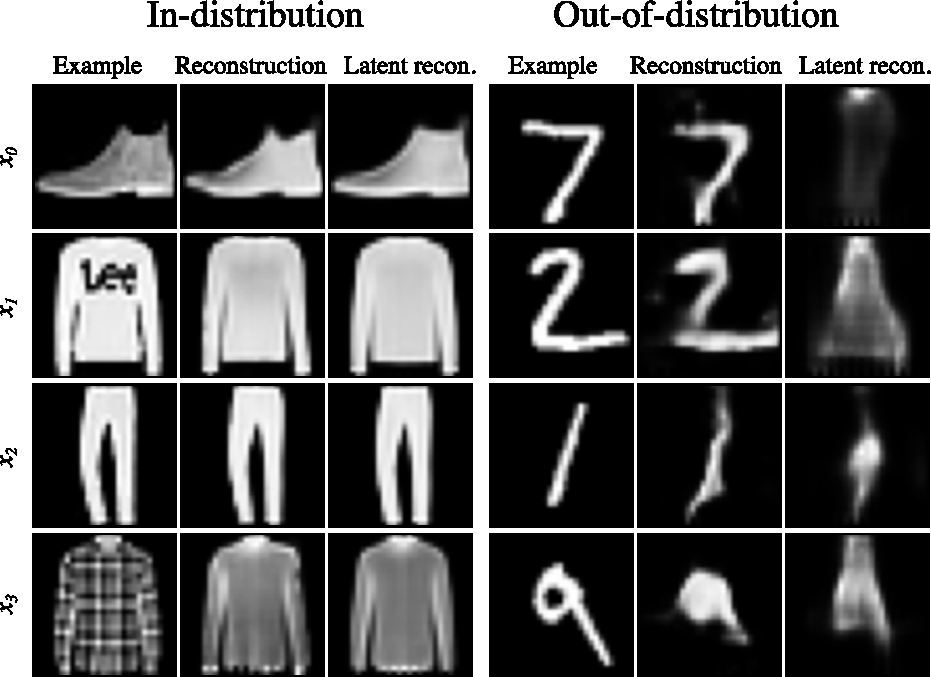
\includegraphics[width=0.7\columnwidth]{paper_hierarchical/reconstructions-front-page-4-samples-2-recons2.pdf}
    \caption[Reconstructions of a hierarchical VAE trained on FashionMNIST.]{%
        Reconstructions using a hierarchical VAE trained on FashionMNIST.
        Reconstruction quality of OOD data is comparable to in-distribution data, resulting in high likelihoods and poor OOD discrimination.
        By sampling the $k$ bottom-most latent variables from the conditional prior distribution $p(\zb_{\geq l}|\zb_{>l})$ (latent reconstructions) instead of the approximate posterior $q(\zb_{>l}|\zb_{<l})$, the model reconstructs from the training distribution resulting in lower $p(\xb|\zb)$ for OOD data.
    }
    \label{fig_hierarchical:reconstructions-fashionmnist}
\end{figure}
% First paragraph: Explains why OOD detection is important in a broad perspective
The reliability and safety of machine learning systems applied in the real-world is contingent on the ability to detect when an input is different from the training distribution. %, an anomaly.
Supervised classifiers built as deep neural networks are well-known to misclassify such \textit{out-of-distribution} (OOD) inputs to known classes with high confidence \cite{goodfellow_explaining_2015, nguyen_deep_2015}.
Several approaches have been suggested to equip deep classifiers with OOD detection capabilities \cite{hendrycks_baseline_2017, lakshminarayanan_simple_2017, hendrycks_deep_2019, devries_learning_2018}.
% However, such methods are inherently supervised and require in-distribution labels or examples of OOD data from an a priori known distribution which limit their applicability.
But, such methods are inherently supervised and require in-distribution labels or examples of OOD data limiting their applicability and generality.

% Second paragraph: Outline deep generative modeling approach and their failure
Unsupervised generative models that estimate an explicit likelihood should understand what it means to be in- and out-of-distribution without requiring labels or examples of OOD data.
By directly modeling the training distribution, such models are expected to assign low likelihoods to OOD data as it originates from regions of little or no support under the learned density \cite{bishop_novelty_1994}.
Recent advances in deep generative models \cite{kingma_autoencoding_2014, rezende_stochastic_2014, oord_pixel_2016, salimans_pixelcnn_2017, kingma_glow_2018} have enabled learning high quality generative models on complex data such as natural images, sequences including audio \cite{oord_wavenet_2016} and graphs \cite{kipf_variational_2016}.
However, recent observations have brought into question the quality of the learned density estimates by showing that they often assign higher likelihoods to OOD data than to in-distribution data \cite{nalisnick_deep_2019, choi_waic_2019}.
Many complex data distributions can be explained to a large degree by low-level features, e.g. edges in images.
However, such features do not explain high-level semantics of the data and may inhibit OOD detection \cite{ren_likelihood_2019, nalisnick_deep_2019}

\textbf{In this paper}, we examine the failure cases of deep generative models on OOD detection tasks within the context of hierarchical VAEs, and make the following contributions:
\begin{itemize}
    \item[(i)] We provide evidence that the root cause of OOD failures is that learned low-level features generalize well across datasets and dominate the estimated likelihoods.
    \item[(ii)] We then propose a fast, scalable, and fully unsupervised likelihood-ratio score for OOD detection that is explicitly developed to ensure that data should be in-distribution across all feature levels, which prevents the low-level features from dominating.
    \item[(iii)] With the likelihood-ratio score, we demonstrate state-of-the-art performance across a wide range of known OOD failure cases.
\end{itemize}


\section{Why does OOD detection fail?}\label{sec_paper_hierarchical:why-does-ood-fail}
\begin{figure}[t]
    \centering
    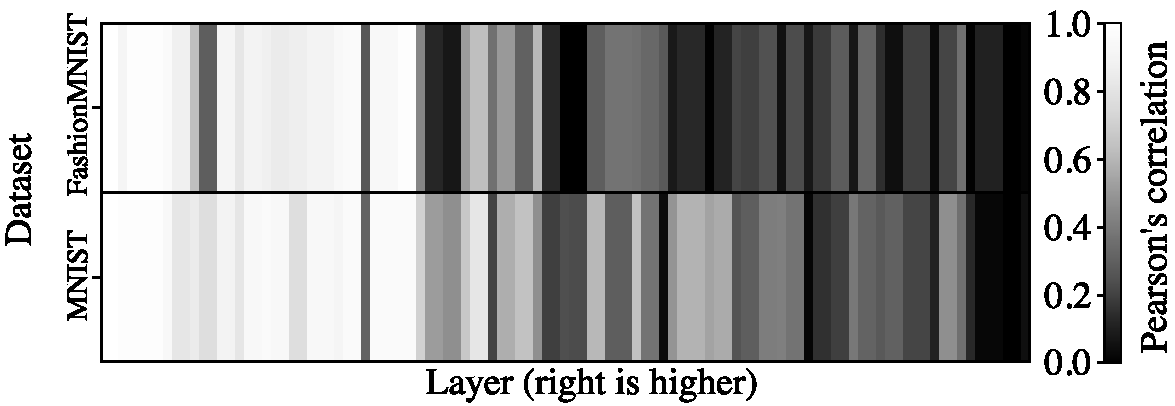
\includegraphics[width=1\columnwidth]{paper_hierarchical/feature-correlation-heatmap2.pdf}
    \vspace{0mm}
    \caption[Absolute correlations between data representations in all layers of the inference network of a hierarchical VAE trained on FashionMNIST and of another trained on MNIST.]{
    Absolute correlations between data representations in all layers of the inference network of a hierarchical VAE trained on FashionMNIST and of another trained on MNIST.
    We compute the correlation between the representations of the two different models given the same data, FashionMNIST (top) and MNIST (bottom).
    %We reduce the representations to a single number by summing over all dimensions and compute the correlation between these numbers for 256 examples.
    %To reduce de-correlation due to the stochastic latent variables, we encode using the mode of the approximate posterior distributions.
    }
    \vspace{0mm}
    \label{fig_hierarchical:correlations-heatmap}
\end{figure}

The inability to detect out-of-distribution data with deep generative models is surprising.
Before the advent of deep generative models, this was not considered a major issue for probabilistic models \cite{bishop_novelty_1994}.
Is the failure due to model pathologies or something different?

Deep learning models are generally believed to form hierarchies of representations that range from low-level features to more conceptual ones related to semantics \cite{bengio_representation_2013}.
This has also been observed within deep generative models \cite{maaloe_biva_2019, child_very_2021}.
%Recent research \cite{maaloe_biva_2019, child_very_2021, vahdat_nvae_2020}, has shown that deep latent variable models are able to learn rich hierarchical representations with increasing levels of abstraction and global structure towards the top of the hierarchy.
For image data there is a trend that the low-level features are quite similar across models (edge detectors, etc.). This raises the question to what extend such features are relevant when detecting OOD data, also suggested  by \cite{nalisnick_deep_2019} and examined for Glow and PixelCNN in \cite{schirrmeister_understanding_2020}.
To investigate, we train two hierarchical VAEs (\cref{sec_paper_hierarchical:background-hie-VAE}) on FashionMNIST and MNIST, respectively, and compute the between-models correlation of the extracted features of in-distribution data and OOD data.
The result appears in \cref{fig_hierarchical:correlations-heatmap}.
We observe that features extracted in the early layers (low-level features) correlate strongly between the two models, and that this correlation drops as we get into later layers.
This suggests that low-level features do not carry much information for OOD detection.

To shed further light on the impact of semantic versus low-level features, we look at model reconstructions of images with a hierarchical VAE (\cref{fig_hierarchical:biva-reconstructions-celeba}).
To study the feature hierarchy, we replace the inference distribution with the corresponding conditional prior in the first layers of the model to see what information is lost.
We observe that as more layers rely on the prior, more details are lost.
Sunglasses, which are uncommon, are first replaced by more common glasses, and then finally disappear.
%Likewise, a long-haired man eventually becomes woman.
This suggests that as we fall back to the conditional priors of each layer, we are pushed closer to local modes of the modeled distribution.

\begin{figure}[t]
    \centering
    %\vspace{0.17cm}
    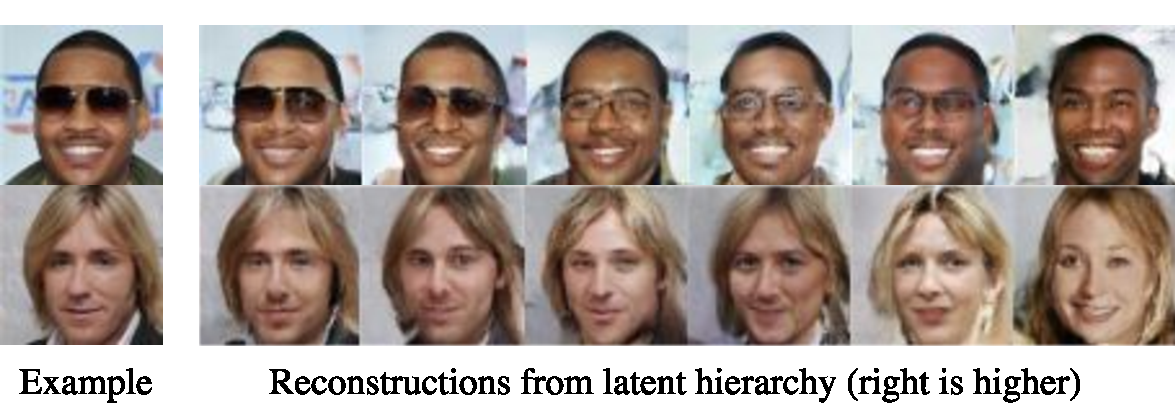
\includegraphics[width=1\columnwidth]{paper_hierarchical/biva_reconstructions.pdf}
    % https://docs.google.com/drawings/d/1UXdA3c18Oek9_env1vEB9mqOAHZ-tu0ijWmvqmapWCk/edit?usp=sharing
    \vspace{0mm}
    \caption[Reconstructions of in-distribution data (CelebA) of the BIVA model using higher latent variables.]{Reconstructions of in-distribution data (CelebA) of the BIVA model using higher latent variables  \cite{maaloe_biva_2019}.
    The higher the latent variable, the more the reconstructions fall into the mode of the learned distribution.
    It is more common to wear regular glasses than sunglasses but most common not to wear glasses at all.
    A man with long hair collapses into the mode of the more common long-haired woman.}
    \vspace{0mm}
    \label{fig_hierarchical:biva-reconstructions-celeba}
\end{figure}
Finally, we look at reconstructions of out-of-distribution data.
\cref{fig_hierarchical:reconstructions-fashionmnist} illustrates that MNIST data is surprisingly well reconstructed by a hierarchical VAE trained on FashionMNIST.
Similar results have been found elsewhere \cite{xiao_likelihood_2020}.
We repeat the previous experiment and replace inference distributions by their corresponding conditional prior, and now observe that reconstructions from higher latent layers become increasingly similar to the data on which the model was trained.
The reliance on conditional priors seems to prevent accurate reconstruction of out-of-distribution data.
Some details are lost on in-distribution data too, but the distinction between that and out-of-distribution data becomes more clear.

\textbf{These observations lead to our main hypothesis.}
The lowest latent variables in a hierarchical VAE learn generic features that can describe a wide range of data.
This enables the model to achieve high rates of compression and high likelihoods, even on out-of-distribution data as long as the learned low-level features are appropriate.
We further suggest that OOD data are in-distribution with respect to these low-level features, but not with respect to semantic ones.

\vspace{0cm}
\section{Background and related work}

\subsection{Variational autoencoders}
The variational autoencoder (VAE) \cite{kingma_autoencoding_2014, rezende_stochastic_2014} is a framework for constructing deep generative models defined by an observed variable $\mathbf{x}$ and a stochastic latent variable $\mathbf{z}$.
Typically, a neural network with parameters $\thetab$ is chosen to parameterize the generative distribution $p_\thetab(\xb,\zb)=p_\thetab(\xb|\zb)p(\zb)$, where the prior $p(\zb)$ is commonly a standard Gaussian $\mathcal{N}(\0, \Ib)$.
The true posterior $p(\zb|\xb)$ is generally not analytically tractable and is approximated by a variational distribution $q_\phib(\zb|\xb)$ parameterized via another neural network with parameters $\phib$. The approximate posterior $q_\phib(\zb|\xb)$ is most often  a diagonal covariance Gaussian.
The model parameters $\thetab$ and variational parameters $\phib$ are jointly optimized by maximizing the \textit{evidence lower bound} (ELBO),
\begin{equation}\label{eq_hierarchical:elbo}
    \log p_\thetab(\xb) \geq \mathbb{E}_{q_\phib(\zb|\xb)} \left[ \log \frac{p_\thetab(\xb,\zb)}{q_\phib(\zb|\xb)} \right] \equiv \mathcal{L}(\xb; \thetab, \phib)\ .
\end{equation}
For brevity, we will denote $\mathcal{L}(\xb; \thetab, \phib)$ as $\mathcal{L}(\xb)$ or $\mathcal{L}$. The reparameterization trick is used to backpropagate gradients through the stochastic latent variables with low variance.

The VAE is defined with a single latent variable which limits the ability to learn a high likelihood representation of complex input distributions, e.g.\ natural images.
There exists a few complementary approaches to make the VAE more flexible: (i) model a more expressive variational distribution $q_\phib(\zb|\xb)$ or prior distribution $p_\thetab(\zb)$ \cite{rezende_variational_2015, kingma_improved_2016}, (ii) model a more expressive posterior distribution $p_\thetab(\xb|\zb)$ e.g. with a autoregressive decoder \cite{oord_conditional_2016} and (iii) learn a deeper hierarchy of latent variables \cite{burda_importance_2016, sonderby_ladder_2016}.
Here, we focus on the latter.


\subsection{Hierarchical variational autoencoders}\label{sec_paper_hierarchical:background-hie-VAE}
Hierarchical VAEs are a family of probabilistic latent variable models which extends the basic VAE by introducing a hierarchy of $L$ latent variables $\zb=\zb_1, \dots, \zb_L$.
The most common generative model is defined from the top down as $p_\thetab(\xb|\zb)=p(\xb|\zb_1)p_\thetab(\zb_1|\zb_2)\cdots p_\thetab(\zb_{L-1}|\zb_L)$.
The inference model can then be defined in two ways respectively referred to as \textit{bottom-up} \cite{burda_importance_2016}
\begin{equation}
    %q_\phib(\zb|\xb)=q_\phib(\zb_1|\xb)q_\phib(\zb_2|\zb_1)\cdots q_\phib(\zb_L|\zb_{L-1})
    q_\phib(\zb|\xb) = q_\phib(\zb_1|\xb)\textstyle\prod_{i=2}^{L} q_\phib(\zb_i|\zb_{i-1})
\end{equation}
and \textit{top-down} \cite{sonderby_ladder_2016}
\begin{equation}
    % q_\phib(\zb|\xb)=q_\phib(\zb_{L}|\xb)q_\phib(\zb_{L-1}|\zb_L)\cdots q_\phib(\zb_2|\zb_1),
    q_\phib(\zb|\xb) = q_\phib(\zb_L|\xb)\textstyle\prod_{i=L-1}^{1} q_\phib(\zb_{i}|\zb_{i+1}) \ .
\end{equation}
Regardless of the choice of inference model, a hierarchical VAE is still trained using the ELBO \cref{eq_hierarchical:elbo}.

Until recently, hierarchical VAEs gave inferior likelihoods compared to state-of-the-art autoregressive \cite{ho_flow_2019} and flow-based models \cite{salimans_pixelcnn_2017}.
This was changed by \textcite{maaloe_biva_2019}, \textcite{vahdat_nvae_2020}, and \textcite{child_very_2021}, which introduced complementary methods to extend the number of latent variables to a very deep hierarchy resulting in state-of-the-art likelihood performance.

In this paper we employ a simple hierarchical VAE with bottom-up inference paths and the more powerful BIVA variant with a bidirectional (top-down and bottom-up) inference model \cite{maaloe_biva_2019}. We employ skip connections between latent variables but omit them for brevity.


\subsection{Out-of-distribution detection}\label{sec_paper_hierarchical:background-ood-detection}
% Intro to alternative scores
So far, no reliable direct likelihood-based method has been found for fully unsupervised deep generative model OOD detection.
A major line of work considers developing new scores that are more reliable than the likelihood.
This includes the \textit{typicality} test presented by \textcite{nalisnick_detecting_2019} which is an OOD detection test based on the typicality of a batch of potentially OOD examples.
This approach however requires a batch of examples from the same class (OOD or not) which limits its practical applicability.
In \textcite{ren_likelihood_2019}, the \textit{likelihood ratio} between a primary model and a background model was shown to be an effective score for OOD detection.
However, to train the background model, the in-distribution data is perturbed via a data augmentation technique that is designed with knowledge about the confounding factors between the in-distribution data and the OOD data. Furthermore, it is tuned towards high performance on a known OOD dataset.
\textcite{serra_input_2020} take a similar approach and attribute the failure to detect OOD data to the high influence of the input complexity on the likelihood and choose a generic lossless compression algorithm as the background model.
Although this method gives good results, no single best choice of compression algorithm exists for all types of OOD data, and any particular choice encodes prior knowledge about the data into the detection method.
Both these methods can be seen as correcting for low-level features of the OOD data being assigned high model likelihood by using a second model focused exclusively on these features.

Similar to these methods, the majority of the approaches to OOD detection make assumptions about the nature of the OOD data.
The assumptions encompass using labels on the in-distribution data \cite{hendrycks_baseline_2017, liang_enhancing_2018, alemi_uncertainty_2018, lee_simple_2018, lakshminarayanan_simple_2017}, examples of OOD data \cite{hendrycks_deep_2019}, augmenting in-distribution data to mimic it \cite{ren_likelihood_2019}, or assuming a certain data type \cite{serra_input_2020}.
Any of these assumptions encode implicit biases into the model about the attributes of OOD data which, in turn, might impair performance on truly unknown data examples (unknown unknowns).

% Introduce the contrast to results with VAEs
While some of these methods achieve very good results on OOD detection with autoregressive models \cite{oord_pixel_2016, salimans_pixelcnn_2017} and invertible flow-based models \cite{kingma_glow_2018}, it was recently shown that they can be much less effective for VAEs \cite{xiao_likelihood_2020} highlighting the need for a more reliable OOD score for VAEs.
Although VAEs have the same failure cases as autoregressive and flow-based models, the caveat is that the difference in the likelihood is generally not as big and reconstructions of OOD can be surprisingly good \cite{xiao_likelihood_2020}.
\textcite{xiao_likelihood_2020} alleviate this by refitting the inference network, as previously proposed by \textcite{cremer_inference_2018, mattei_refit_2018}, to a potentially OOD example and measuring the so-called \textit{likelihood regret}.
However, refitting the inference network can be computationally expensive, especially for the large hierarchical VAEs that are used to model complex data \cite{maaloe_biva_2019, vahdat_nvae_2020, child_very_2021}. Furthermore, this scales poorly to large amounts of potentially OOD examples as the optimization is done per example.

A few methods have approached OOD detection in a completely unsupervised fashion \cite{maaloe_biva_2019, choi_waic_2019, xiao_likelihood_2020}.
The work of \textcite{maaloe_biva_2019} is the most related to ours. They introduce BIVA, a deep hierarchy of stochastic latent variables with a top-down and bottom-up inference model and achieve state-of-the-art likelihood scores. 
They also provide early results indicative that a looser likelihood bound may have value in OOD detection.
In this paper, we provide an explanation of those results, and significantly improve upon them.


\section{OOD detection with hierarchical VAEs}
\subsection{A bound for semantic OOD detection}
If the lowest latent variable in the VAE hierarchy codes for a large part of the low-level features required to reconstruct the input with high accuracy, as exemplified in \cref{fig_hierarchical:reconstructions-fashionmnist}-\ref{fig_hierarchical:biva-reconstructions-celeba}, then $p_\thetab(\xb|\zb_1)$ will be high for both in- and out-of-distribution data.
Hence, any OOD detection capabilities based on the ELBO $\mathcal{L} = \mathbb{E}_{q_\phib(\zb|\xb)}[\log p_\thetab(\xb|\zb_1)] - D_{\mathrm{KL}}( q_\phib(\zb|\xb) || p(\zb))$ from \cref{eq_hierarchical:elbo} relies on the KL-term for OOD detection. For a bottom-up hierarchical VAE, the KL-term $D_{\mathrm{KL}}( q_\phib(\zb|\xb) || p(\zb))$ can be expressed by a hierarchical sum% over the hierarchy
% \begin{multline}
%     \mathcal{L}(\xb) =  \mathbb{E}_{q_\phib(\zb|\xb)} \Big[ \log p_\thetab(\xb|\zb_1) \\
%                      + \textstyle\sum_{i=1}^{L-1} \log \frac{p_\thetab(\zb_i|\zb_{i+1})}{q_\phib(\zb_i|\zb_{i-1})} 
%                      + \log \frac{p_\thetab(\zb_L)}{q_\phib(\zb_L|\zb_{L-1})} \Big] .
% \end{multline}
% \begin{multline}
%     D_{\mathrm{KL}}( q(\zb|\xb) || p(\zb)) = \\
%     \mathbb{E}_{q_\phib(\zb|\xb)} \Big[ \textstyle\sum_{i=1}^{L-1} \log \frac{p_\thetab(\zb_i|\zb_{i+1})}{q_\phib(\zb_i|\zb_{i-1})} + \log \frac{p_\thetab(\zb_L)}{q_\phib(\zb_L|\zb_{L-1})} \Big] .
% \end{multline}
\begin{equation}
    \mathbb{E}_{q_\phib(\zb|\xb)} \Big[ \textstyle\sum_{i=1}^{L-1} \log \frac{p_\thetab(\zb_i|\zb_{i+1})}{q_\phib(\zb_i|\zb_{i-1})} + \log \frac{p_\thetab(\zb_L)}{q_\phib(\zb_L|\zb_{L-1})} \Big] \ .
\end{equation}
In general, the absolute log-ratios grow with $\mathrm{dim}(\zb_i)$ as the individual log probability terms are computed by summing over the dimensionality of $\zb_i$.
This means that the value of the KL-term is dominated by terms where $\zb_i$ is high-dimensional. We refer to Appendix C for a more detailed argument.
Since hierarchical VAEs are generally constructed with a bottleneck type structure, the terms corresponding to latent variables towards the top of the hierarchy will have a vanishing influence on the value of the KL-term.
However, as the semantic information most relevant for OOD detection has a tendency to be represented in the top-most latent variables, this makes OOD detection using the regular ELBO difficult, even for state-of-the-art models.
This behavior has also been reported by \textcite{xiao_likelihood_2020}.

To shift the ELBO from primarily being based on the approximate posterior of the lowest latent variables to instead focus on the conditional prior, \textcite{maaloe_biva_2019} introduced slightly different likelihood lower bound defined as
\begin{equation}\label{eq_hierarchical:biva->k}
    \mathcal{L}^{>k} = \mathbb{E}_{p_\thetab(\zb_{\leq k}|\zb_{>k}) q_\phib(\zb_{>k}|\xb)} \left[ \log \frac{p_\thetab(\xb|\zb)p_\thetab(\zb_{>k})}{q_\phib(\zb_{>k}|\xb)} \right]
\end{equation}
where $k\in\{0,1,\dots,L\}$ (see Appendix for the derivation).
We note that $\mathcal{L}^{>0}$ is the regular ELBO (\cref{eq_hierarchical:elbo}) and that empirically we always observe that $\mathcal{L}\geq\mathcal{L}^{>k} \, \forall \, k$ although this need not hold in general.
The core idea behind this variation on the ELBO is to sample the $k$ lowest latent variables from the conditional prior $\zb_1,\dots,\zb_l \sim p_\thetab(\zb_{\leq k}|\zb_{>k})$ and only the $L-k$ highest from the approximate posterior $\zb_{k+1},\dots,\zb_L \sim q_\phib(\zb_{>k}|\xb)$.
Importantly, this has the effect that the data likelihood $p(\xb|\zb)$ is dependent on the approximate posterior through a latent variable $\zb_{k+1}$ different from $\zb_1$ for all $k \geq 1$.
Thereby, the likelihood can be evaluated with a reconstruction from each of the latent variables $\zb_k$ of the hierarchical VAE.
Hence, we can now test how well the input $\xb$ is reconstructed from each latent variable.
The notation $\mathcal{L}^{>k}$ highlights that for latent variables $\zb_{>k}$, the bound is the regular ELBO while for the latent variables $\zb_{\leq k}$, the bound is evaluated using the (conditional) prior rather than the approximate posterior as the proposal distribution.


\subsection{A likelihood-ratio score for all feature levels}
While the $\mathcal{L}^{>k}$ bound provides a score for performing semantic OOD detection, it still relies on the data space likelihood function (see equation \cref{eq_hierarchical:likelihoods-as-exact} below), which is known to be problematic for OOD detection (\cref{sec_paper_hierarchical:background-ood-detection}). To alleviate this, we phrase OOD detection as a likelihood ratio test of being \emph{semantically} in-distribution.
A standard likelihood ratio test \cite{buse_likelihood_1982} suggests to consider the ratio between the associated likelihoods, which we can approximate on a log-scale by the corresponding lower bounds $\mathcal{L}$ and $\mathcal{L}^{>k}$,
\begin{equation}\label{eq_hierarchical:llr-as-difference-in-likelihoods}
    % LLR = - 2 log(L0 / L1)
    % where L0 < L1 so log(L0 / L1) < 0 and LLR > 0
    % LLR = 2 log(L1 / L0)
    %     = 2 (log(L1) - log(L0))
    %     = 2 (ELBO - L^{>k})  % LLR^{>a,>b} where a=0
    % L1 = ELBO
    % L0 = L^{>k}
    LLR^{>k}(\xb) = \mathcal{L}(\xb) - \mathcal{L}^{>k}(\xb) \ .
\end{equation}
%This likelihood ratio contrasts the ELBO with $\mathcal{L}^{>k}$ for a variable choice of $k$.
Since, empirically, $\mathcal{L}\geq\mathcal{L}^{>k}$, the ratio is always positive as is standard for likelihood ratio tests.
A low value of $LLR^{>k}(\xb)$ means that the ELBO and $\mathcal{L}^{>k}$ are almost equally tight for the data.
On the contrary, a high value indicates that $\mathcal{L}^{>k}$ is looser on the data than the ELBO; hence, the data may be OOD.


We can gather further insights about this score if we write the regular ELBO and the $\mathcal{L}^{>k}$ bounds in the exact form that includes the intractable KL-divergence between the approximate and true posteriors,
\begin{align}
    \mathcal{L}      &= \log p_\thetab(\xb) - D_{\mathrm{KL}}\left( q_\phib(\zb|\xb) || p_\thetab(\zb|\xb)\right), \label{eq_hierarchical:likelihoods-as-exact} \\ 
    \mathcal{L}^{>k} &= \log p_\thetab(\xb) - D_{\mathrm{KL}}\left( p_\thetab(\zb_{\leq k }|\zb_{>k}) q_\phib(\zb_{>k}|\xb) || p_\thetab(\zb|\xb)\right) \nonumber \ .
\end{align}
Subtracting these cancel out the two data likelihood terms $\log p_\thetab(\xb)$ and only the KL-divergences from the approximate to the true posterior remain,
\begin{align}
    LLR^{>k}(\xb) &= - D_{\mathrm{KL}}\left( q_\phib(\zb|\xb) || p_\thetab(\zb|\xb)\right) \\
                 &\quad + D_{\mathrm{KL}}\left( p_\thetab(\zb_{\leq k}|\zb_{>k}) q_\phib(\zb_{>k}|\xb) || p_\thetab(\zb|\xb)\right) \ . \notag
\end{align}\label{eq_hierarchical:llr-as-kls}

Hence, it is clear that compared to the likelihood bound $\mathcal{L}^{>k}$, this likelihood-ratio measures divergence exclusively in the latent space whereas $\mathcal{L}^{>k}$ includes the $\log p_\thetab(\xb)$ term similar to the ELBO.
Therefore, the $LLR^{>k}$ score should be an improved method for semantic OOD detection compared to $\mathcal{L}^{>k}$.
Now, it can be noted that if we replace the regular ELBO, $\mathcal{L}$, in \cref{eq_hierarchical:likelihoods-as-exact} with the strictly tighter importance weighted bound \cite{burda_importance_2016},
\begin{equation}
    \mathcal{L}_{S} = \mathbb{E}_{q(\zb|\xb)}\left[ \log \frac{1}{N} \sum_{s=1}^{S} \frac{p(\xb, \zb^{(s)})}{q(\zb^{(s)}|\xb)} \right] \ , \label{eq_hierarchical:iw-bound}
\end{equation}
then, in the limit $S\rightarrow\infty$, we have $\mathcal{L}_{S} \rightarrow \log p_\thetab(\xb)$ and the likelihood ratio reduces to
\begin{equation}
    LLR^{>k}_{S}(\xb) \rightarrow D_{\mathrm{KL}}( p(\zb_{\leq k}|\zb_{>k}) q(\zb_{>k}|\xb) || p(\zb|\xb))
\end{equation}\label{eq_hierarchical:llr-as-kls-iwae-reduced}
which, in practice, is well-approximated for a finite $S$. We expect this importance weighted likelihood ratio to monotonically improve upon the one in \cref{eq_hierarchical:llr-as-kls} as $S$ increases and the KL-divergence in the regular ELBO that contains terms for which $\zb_i$ is high-dimensional goes to zero.


Since the scores in \cref{eq_hierarchical:llr-as-kls,eq_hierarchical:llr-as-kls-iwae-reduced} are estimated by sampling their estimators are stochastic objects with nonzero variance.
We note that $\text{Var}(\widehat{LLR}^{>k}) = \text{Var}(\hat{\mathcal{L}}) + \text{Var}(\hat{\mathcal{L}}^{>k}) - 2\, \text{Cov}(\hat{\mathcal{L}}, \hat{\mathcal{L}}^{>k})$.
Since $\log p_\thetab(\xb)$ and part of the KL divergence are identical in the expressions of $\mathcal{L}$ and $\mathcal{L}^{>k}$ we expect $\text{Cov}(\hat{\mathcal{L}}, \hat{\mathcal{L}}^{>k})$ to be positive which reduces the total variance. 
Empirical results indeed show that $\text{Var}(\widehat{LLR}^{>k})$ is larger than $\text{Var}(\hat{\mathcal{L}})$ but smaller than $\text{Var}(\hat{\mathcal{L}}^{>k})$.
%Whether this decreases the variance to below the variance of any of the two bounds, we do not know, and we believe it to be difficult to verify mathematically.
Nevertheless, the variance of the estimators is guaranteed to go to zero as the number of samples is increased.

The OOD scores considered in this research all assume that what discriminates an out-of-distribution from an in-distribution data point are semantic, high-level features. Clearly, if this is not the case and the difference instead lies in low-level statistics, the scores would likely fail. We hypothesize that a complementary bound to \cref{eq_hierarchical:biva->k}, $\mathcal{L}^{<l}$ described in Appendix E, might be useful in these cases, but leave further examination to future work.


\section{Experimental setup}

\paragraph{Tasks} We follow existing literature \cite{nalisnick_deep_2019, hendrycks_deep_2019} and evaluate our method by setting up OOD detection tasks from FashionMNIST \cite{xiao_fashionmnist_2017} to MNIST \cite{lecun_gradientbased_1998} and from CIFAR10 \cite{krizhevsky_learning_2009} to SVHN \cite{netzer_reading_2011}.
For each experiment we train our model on the train split of the former dataset and test its ability to recognize the test split of the latter dataset as OOD from the test split of the former dataset.
We use the standard train/test splits for the datasets.
More details on the datasets can be found in the Appendix.


% Our model
%\begin{wrapfigure}{R}{0.5\columnwidth}
% \begin{SCfigure}[50][t!]
\begin{figure}[t]
    %\begin{figure}
    \centering
    \resizebox{0.25\textwidth}{!}{
    \tikz{
        % inference
        % nodes
        \node[obs] (x_inf) {$\xb$};%
        \node[latent,above=.75cm of x_inf](z1_inf){$\zb_1$}; %
        \node[latent,above=.75cm of z1_inf](z2_inf){$\zb_2$}; %
        % \node[latent,above=.75cm of z2_inf](z3_inf){$\zb_3$}; %
        \node[above=of z2_inf, yshift=-1.cm] (phi) {$q_\phib(\zb|\xb)$}; 
        
        % edges
        \edge[]{x_inf}{z1_inf};
        \edge[]{z1_inf}{z2_inf};
        % \edge[]{z2_inf}{z3_inf};
        \edge[dashed, bend left]{x_inf}{z2_inf};
        % \edge[dashed, bend left]{x_inf}{z3_inf};
        
        % generative
        % nodes$
        \node[obs,right=0.75cm of x_inf] (x_gen) {$\xb$};%
        \node[latent,above=.75cm of x_gen](z1_gen){$\zb_1$}; %
        \node[latent,above=.75cm of z1_gen](z2_gen){$\zb_2$}; %
        % \node[latent,above=.75cm of z2_gen](z3_gen){$\zb_3$}; %
        \node[above=of z2_gen, yshift=-1.cm] (theta) {$p_\thetab(\xb,\zb)$}; 
        
        % edges
        % \edge[]{z3_gen}{z2_gen};
        \edge[]{z2_gen}{z1_gen};
        \edge[]{z1_gen}{x_gen};
        \edge[dashed, bend left]{z2_gen}{x_gen};
        % \edge[dashed, bend left]{z3_gen}{x_gen};
    }
    }
    \caption[Inference and generative models for a bottom-up hierarchical VAEs.]{The inference and generative models, $q_\phib$ and $p_\thetab$, for an $L=2$ layered bottom-up hierarchical VAE as the one used in our experiments.
    Dashed lines indicate deterministic skip connections which are employed in both networks. Skip connections are found to be useful for optimizing latent variable models \cite{dieng_avoiding_2019, maaloe_biva_2019}.}
    \label{fig_hierarchical:hvae-graphical-model}
    % \end{figure}
%\end{wrapfigure}
% \end{SCfigure}
\end{figure}


\paragraph{Models} For each OOD task, we train a simple bottom-up hierarchical VAE with $L$ stochastic layers which we will refer to as ``HVAE''.
To alleviate posterior collapse we include skip-connections that connect $\zb_i$ to $\zb_{i+2}$ for $i\in\{0, L-2\}$ and $\zb_0\equiv\xb$ in both the inference and generative models \cite{dieng_avoiding_2019} and employ the \textit{free bits} scheme with $\lambda=2$ \cite{kingma_improved_2016}.
We use weight-normalization \cite{salimans_weight_2016} on all weights and residual networks in the deterministic paths. 
A graphical representation of this model can be seen in \cref{fig_hierarchical:hvae-graphical-model}.
We use a Bernoulli output distribution for FashionMNIST/MNIST and a discretized mixture of logistics output distribution \cite{salimans_pixelcnn_2017} for CIFAR10/SVHN.
We use $L=3$ for grey-scale images and $L=4$ for natural images.
% For CIFAR/SVHN, we also train a BIVA model \cite{maaloe_biva_2019} with $L=10$ and similar configuration as used by the original paper\footnote{Code available at \url{github.com/larsmaaloee/BIVA} and \url{github.com/vlievin/biva-pytorch}}.
Full model details are in the Appendix.


% Baselines
\paragraph{Baselines} We group baselines into those that use prior knowledge about OOD data, ones that use labels associated with the in-distribution data and purely unsupervised approaches that do not make such assumptions.
Our method falls into the latter category.
For more information on each baseline, we refer to the original literature.


% Metrics and Evaluation
\paragraph{Evaluation} Following previous work \cite{hendrycks_baseline_2017, hendrycks_deep_2019, alemi_uncertainty_2018, ren_likelihood_2019, choi_waic_2019} we use the threshold-independent evaluation metrics of Area Under the Receiver Operator Characteristic (AUROC$\uparrow$), Area Under the Precision Recall Curve (AUPRC$\uparrow$) and False Positive Rate at 80\% true positive rate (FPR80$\downarrow$) where the arrow indicates the direction of improvement.
Note that these metrics are only computable given examples of OOD data but faced with truly OOD data (unknown unknowns), there are many ways to select thresholds to use in practice e.g.\ as the one that yields a specific tolerable false positive rate on the in-distribution test data.
To compute the metrics, we use an equal number of samples from the in-distribution and OOD datasets by including all examples in the smallest of the two sets and randomly sampling equally many from the larger. We compute the $LLR^{>k}$ score with one and $S$ importance samples denoted by $LLR^{>k}_S$.

% The value of k
\paragraph{Selection of $k$} To determine whether an example is OOD in practice, the value of $LLR^{>k}$ is computed on the in-distribution test set for all $k$ and the resulting empirical distribution is used as reference.
If for any value of $k$, the $LLR^{>k}$ score of a new input differs significantly from the empirical distribution, it is regarded OOD.
If it differs for multiple values of $k$, the value for which it differs the most is selected.
In our experiments, we consider an entire dataset at a time and report the results of $LLR^{>k}$ with the value of $k$ that yielded the highest AUROC$\uparrow$ for that dataset in a threshold-free manner.
In practice, slightly better performance may be achieved by choosing $k$ per example.
This would not exclude the use of batching in our method, since $LLR^{>k}$ is computed after the forward pass.


\section{Results}

The likelihoods for our trained models are in \cref{tab_hierarchical:bits-per-dim-ood} alongside baseline results for in-distribution and OOD data.
The main results of the paper on the OOD tasks can be seen along with comparisons to the baseline methods in \cref{tab_hierarchical:rocauc-ood}.
We note that for all our results, the value of the score ($\mathcal{L}^{>k}$ and $LLR^{>k}$) for the training and test splits of the in-distribution data was observed to have the same empirical distribution to within sampling error hence yielding an AUROC score of $\approx0.5$ as expected.
Results on additional commonly used datasets are found in Appendix G.


\begin{table}[t!]
    \centering
    \resizebox{0.8\columnwidth}{!}{%
    \begin{tabular}{lrrrrr}
        \toprule
         Method & Dataset & \multicolumn{4}{c}{Avg. bits/dim}\\
        %   & & $\log p(x)$ & $\mathcal{L}^{>k_1}$ & $\mathcal{L}^{>k_2}$ & $\mathcal{L}^{>k_3}$\\
          & & $\log p(x)$ & $\mathcal{L}^{>1}$ & $\mathcal{L}^{>2}$ & $\mathcal{L}^{>3}$\\
         \midrule
         \multicolumn{6}{c}{\textbf{Trained on FashionMNIST}} \\
         \midrule
         \multirow{2}{*}{Glow}
            & FashionMNIST & 2.96 & - & - & \\
            & MNIST & 1.83 & - & - & \\
         \multirow{2}{*}{HVAE (Ours)}
            & FashionMNIST & 0.420 & 0.476 & 0.579 & - \\
            & MNIST & 0.317 & 0.601 & 0.881 & - \\
         \midrule
         \multicolumn{6}{c}{\textbf{Trained on CIFAR10}} \\
         \midrule
         \multirow{2}{*}{Glow}
          & CIFAR10 & 3.46 & - & - & \\
          & SVHN & 2.39 & - & - & \\
         \multirow{2}{*}{HVAE (Ours)}
            & CIFAR10 & 3.74 & 17.8 & 54.3 & 75.7 \\  % log p(x) = 8010.03
            & SVHN & 2.62 & 10.2 & 64.0 & 93.9 \\
         \multirow{2}{*}{BIVA (Ours)}
          & CIFAR10 & 3.46 & 8.74 & 19.7 & 37.3 \\
          & SVHN & 2.35 & 6.62 & 25.1 & 59.0 \\
         \bottomrule
    \end{tabular}
    }
    \caption[Average bits per dimension of different datasets for generative models trained on FashionMNIST and CIFAR10.]{%
    Average bits per dimension of different datasets for models trained on FashionMNIST and CIFAR10.
    For the hierarchical models we include the $\mathcal{L}^{>k}$ bounds.
    The likelihoods of training and test splits of the in-distribution data are all cases close.
    Since we train on dynamically binarized FashionMNIST, our bits/dim are smaller than for Glow.
    As $k$ is increased for the $L^{>k}$ bound, the bound gets looser but the model eventually assigns higher likelihood to the in distribution data than to the OOD data.
    Glow refers to \textcite{kingma_glow_2018, nalisnick_deep_2019}.
    BIVA refers to our implementation of \textcite{maaloe_biva_2019}.}
    \label{tab_hierarchical:bits-per-dim-ood}
    \vspace{0mm}
\end{table}

\footnotetext{%
    \textcite{serra_input_2020} performs the best when high likelihoods are assigned to OOD data such that the overlap with in-distribution data is low.
    Performance is worse when the overlap is high, cf. \textcite[Table 1]{serra_input_2020}, as seen with complex images.}
\begin{table}[t!]
    \centering
    \resizebox*{!}{0.9\textheight}{%
    \begin{tabular}{lrrr}
        \toprule
         Method & AUROC$\uparrow$ & AUPRC$\uparrow$ & FPR80$\downarrow$ \\
         \midrule
         \multicolumn{4}{c}{\textbf{FashionMNIST (in) / MNIST (out)}} \\
         \midrule
         \multicolumn{4}{l}{\textbf{Use prior knowledge of OOD}} \\
Backgr. contrast. LR (PixelCNN) {\cite{ren_likelihood_2019}}               & $0.994$ & $0.993$ & $0.001$ \\
Backgr. contrast. LR (VAE) {\cite{choi_waic_2019}}                    & $0.924$ & - & - \\
Binary classifier {\cite{ren_likelihood_2019}}                              & $0.455$ & $0.505$ & $0.886$ \\ % 6
$p(\hat{y} | \xb)$ with OOD as noise class {\cite{ren_likelihood_2019}}     & $0.877$ & $0.871$ & $0.195$ \\ % 7
$p(\hat{y} | \xb)$ with calibration on OOD {\cite{ren_likelihood_2019}}     & $0.904$ & $0.895$ & $0.139$ \\ % 8
Input complexity ($S$, Glow) \cite{hendrycks_deep_2019}                    & $0.998$ & - & - \\
Input complexity ($S$, PixelCNN++) \cite{hendrycks_deep_2019}              & $0.967$ & - & - \\
         \multicolumn{4}{l}{\textbf{Use in-distribution data labels $y$}} \\
$p(\hat{y} | \xb)$ {\cite{ren_likelihood_2019, hendrycks_baseline_2017}}                        & $0.734$ & $0.702$ & $0.506$ \\
Entropy of $p(y | \xb)$ {\cite{ren_likelihood_2019}}                        & $0.746$ & $0.726$ & $0.448$ \\
ODIN {\cite{ren_likelihood_2019, liang_enhancing_2018}}                                       & $0.752$ & $0.763$ & $0.432$ \\
VIB \cite{alemi_uncertainty_2018, choi_waic_2019}                                          & $0.941$ & - & - \\
Mahalanobis distance, CNN {\cite{ren_likelihood_2019}}                     & $0.942$ & $0.928$ & $0.088$ \\
Mahalanobis distance, DenseNet {\cite{lee_simple_2018}}                & $0.986$ & - & - \\
Ensemble, 20 classifiers {\cite{ren_likelihood_2019, lakshminarayanan_simple_2017}}                  & $0.857$ & $0.849$ & $0.240$ \\
         \multicolumn{4}{l}{\textbf{No OOD-specific assumptions}} \\
         \multicolumn{4}{l}{\textit{- Ensembles}} \\
WAIC, 5 models, VAE {\cite{choi_waic_2019}}                          & $0.766$ & - & - \\
WAIC, 5 models, PixelCNN {\cite{ren_likelihood_2019}}                      & $0.221$ & $0.401$ & $0.911$ \\
        \multicolumn{4}{l}{\textit{- Not ensembles}} \\
Likelihood regret \cite{xiao_likelihood_2020}                               & $\mathbf{0.988}$ & - & - \\
$\mathcal{L}^{>0}$ + HVAE (ours)                    & $0.268$ & $0.363$ & $0.882$ \\
$\mathcal{L}^{>1}$ + HVAE (ours)                    & $0.593$ & $0.591$ & $0.658$ \\
$\mathcal{L}^{>2}$ + HVAE (ours)                    & $0.712$ & $0.750$ & $0.548$ \\
$LLR^{>1}$ + HVAE (ours)                            & $0.964$ & $0.961$ & $0.036$ \\
$LLR^{>1}_{250}$ + HVAE (ours)                      & $0.984$ & $\mathbf{0.984}$ & $\mathbf{0.013}$ \\
         \midrule
         \multicolumn{4}{c}{\textbf{CIFAR10 (in) / SVHN (out)}} \\
         \midrule
         \multicolumn{4}{l}{\textbf{Use prior knowledge of OOD}} \\
Backgr. contrast. LR (PixelCNN) {\cite{ren_likelihood_2019}}               & $0.930$ & $0.881$ & $0.066$ \\
Backgr. contrast. LR (VAE) {\cite{xiao_likelihood_2020}}                    & $0.265$ & - & - \\
Outlier exposure {\cite{hendrycks_deep_2019}}                              & $0.984$ & - & - \\
Input complexity ($S$, Glow) \cite{serra_input_2020}                   & $0.950$ & - & - \\
Input complexity ($S$, PixelCNN++) \cite{serra_input_2020}             & $0.929$ & - & - \\
Input complexity ($S$, HVAE) (Ours) \cite{serra_input_2020}\footnotemark & $0.833$ & $0.855$ & $0.344$ \\
         \multicolumn{4}{l}{\textbf{Use in-distribution data labels $y$}} \\
Mahalanobis distance {\cite{lee_simple_2018}}                          & $0.991$ & - & -  \\
         \multicolumn{4}{l}{\textbf{No OOD-specific assumptions}} \\
         \multicolumn{4}{l}{\textit{- Ensembles}} \\
WAIC, 5 models, Glow {\cite{choi_waic_2019}}                          & $1.000$ & - & - \\
WAIC, 5 models, PixelCNN {\cite{ren_likelihood_2019}}                      & $0.628$ & $0.616$ & $0.657$ \\
         \multicolumn{4}{l}{\textit{- Not ensembles}} \\
Likelihood regret \cite{xiao_likelihood_2020}                               & $0.875$ & - & - \\
$LLR^{>2}$ + HVAE (ours)                            & $0.811$ & $0.837$ & $0.394$ \\
$LLR^{>2}$ + BIVA (ours)                            & $\mathbf{0.891}$ & $\mathbf{0.875}$ & $\mathbf{0.172}$ \\
         \bottomrule
    \end{tabular}%
    }
    \caption[AUROC, AUPRC, and FPR80 of generative models for OOD detection (MNIST/FashionMNIST and SVHN/CIFAR10).]{%
        AUROC$\uparrow$, AUPRC$\uparrow$ and FPR80$\downarrow$ for OOD detection for a FashionMNIST model using scores on the FashionMNIST test set as reference. We bold the best results within the "No OOD-specific assumptions" group since we only compare directly to those.
        HVAE (ours) refers to our hierarchical bottom-up VAE.
        BIVA (ours) refers to our implementation of the hierarchical BIVA model \cite{maaloe_biva_2019}.
    }
    \label{tab_hierarchical:rocauc-ood}
\end{table}


\subsection{Likelihood-based OOD detection}
% \begin{sidewaysfigure}
\begin{figure}
    %\captionstyle{centerlast}
    \centering
    \begin{subfigure}[l]{0.48\columnwidth}
        \centering
        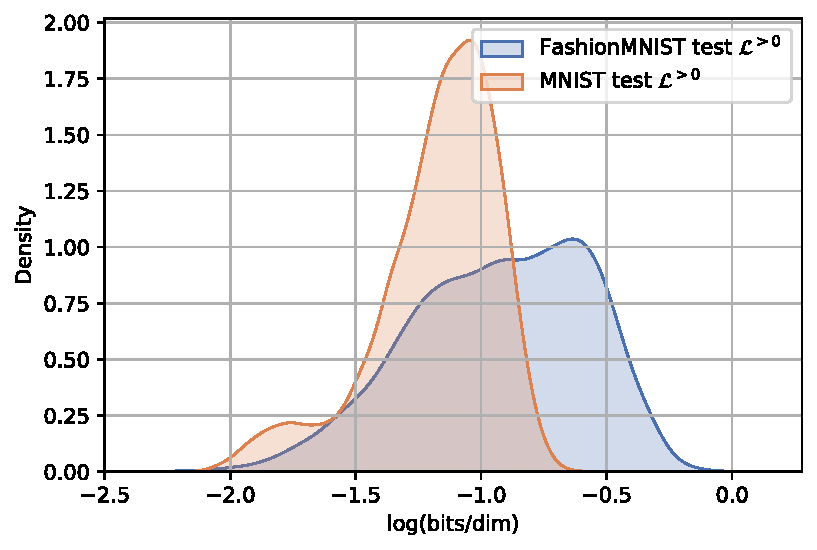
\includegraphics[width=1\columnwidth]{paper_hierarchical/densities-FashionMNIST-test-MNIST-test-bpp-k-0_sohau.pdf}
        \caption{}
        \label{fig_hierarchical:FMNIST-elbo-k0}
    \end{subfigure}
    % \hfill
    \begin{subfigure}[c]{0.48\columnwidth}
        \centering
        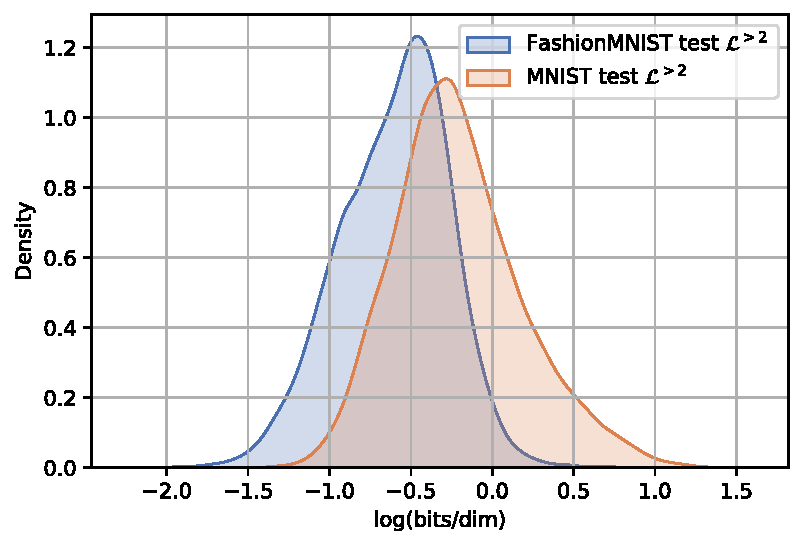
\includegraphics[width=1\columnwidth]{paper_hierarchical/densities-FashionMNIST-test-MNIST-test-bpp-k-2_sohau.pdf}
        \caption{}
        \label{fig_hierarchical:FMNIST-elbo-k2}
    \end{subfigure}
    % \hfill
    \begin{subfigure}[r]{0.48\columnwidth}
        \centering
        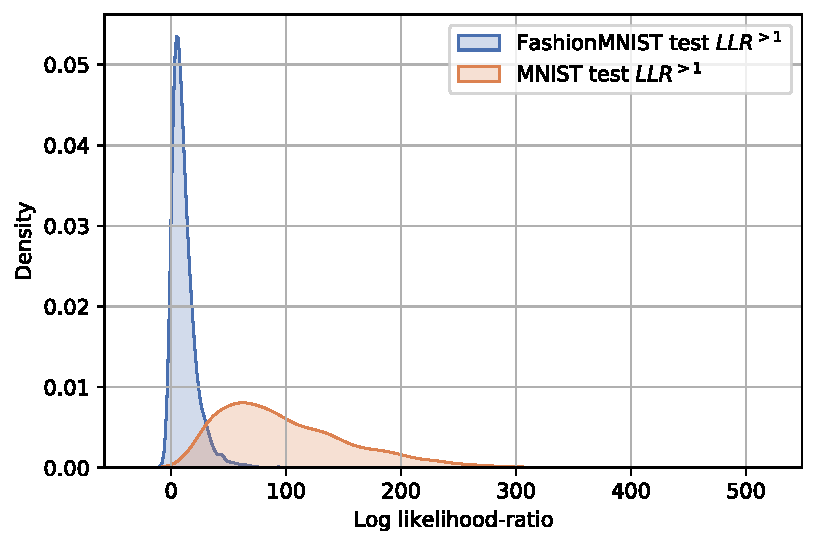
\includegraphics[width=1\columnwidth]{paper_hierarchical/densities-FashionMNIST-test-MNIST-test-LLR-0-1_sohau.pdf}
        \caption{}
        \label{fig_hierarchical:FMNIST-llr}
    \end{subfigure}
    \caption[Empirical densities of FashionMNIST (in-distribution) and MNIST (OOD) using the raw likelihood and $\mathcal{L}^{>2}$ bound.]{%
    Empirical densities of FashionMNIST (in-distribution) and MNIST (OOD) using the raw likelihood \subref{fig_hierarchical:FMNIST-elbo-k0}, the $\mathcal{L}^{>2}$ bound \subref{fig_hierarchical:FMNIST-elbo-k2} and the $LLR^{>1}$ score \subref{fig_hierarchical:FMNIST-llr}. All densities are computed using the HVAE model.
    For the regular likelihood MNIST is very clearly more likely on average than the FashionMNIST test data while with the $\mathcal{L}^{>2}$ bound separation is better but significant overlap remains.
    The $LLR^{>1}$ provides a high degree of separation. Likelihoods are reported in units of the natural log of the number of bits per dimension.
    }
    \label{fig_hierarchical:FMNIST-ood-densities}
\end{figure}
% \end{sidewaysfigure}

We first report the results of the different variations of the $\mathcal{L}^{>k}$ bound for OOD detection. 
We reconfirm the results of \textcite{nalisnick_deep_2019} by observing that our hierarchical latent variable models also assign higher $\mathcal{L}^{>0}$ to the OOD dataset in the FashionMNIST/MNIST and CIFAR10/SVHN cases resulting in an AUROC$\uparrow$ inferior to random (\cref{tab_hierarchical:rocauc-ood}).
Switching the in-distribution data for the OOD data in both cases result in correctly detecting the OOD data; an asymmetry also reported by \textcite{nalisnick_deep_2019}.
\cref{fig_hierarchical:FMNIST-elbo-k0} shows the density of $\mathcal{L}^{>0}$ in bits per dimension \cite{theis_note_2016} by the model trained on FashionMNIST when evaluated on the FashionMNIST and MNIST test sets.
We observe a high degree of overlap, with less separation of the OOD data compared to similar results of autoregressive and flow-based models, like \textcite{xiao_likelihood_2020}.


We then evaluate the looser $\mathcal{L}^{>k}$ \cref{eq_hierarchical:biva->k} for $k\in\{1,L\}$.
\cref{fig_hierarchical:FMNIST-elbo-k2} shows the result for $\mathcal{L}^{>2}$, which yielded the highest AUCROC$\uparrow$, only slightly better than random.
Like \textcite{maaloe_biva_2019}, we see that increasing the value of $k$ generally leads to improved OOD detection.
However, we also observe that the two empirical distributions never cease to overlap.
Importantly, depending on the OOD dataset, the amount of remaining overlap can be high which limits the discriminatory power of the likelihood-based $\mathcal{L}^{>k}$ bound.
This is in-line with the pathological behavior of the raw likelihood of latent variable models when used for OOD detection \cite{xiao_likelihood_2020}.
Since a high degree of overlap also seems present in \textcite{maaloe_biva_2019}, and we see the same problem for our BIVA model trained on CIFAR10, we do not expect this to be due to the less expressive HVAE.


\subsection{Likelihood-ratio-based OOD detection}
\begin{figure}
    \centering
    \begin{subfigure}[l]{0.495\columnwidth}
        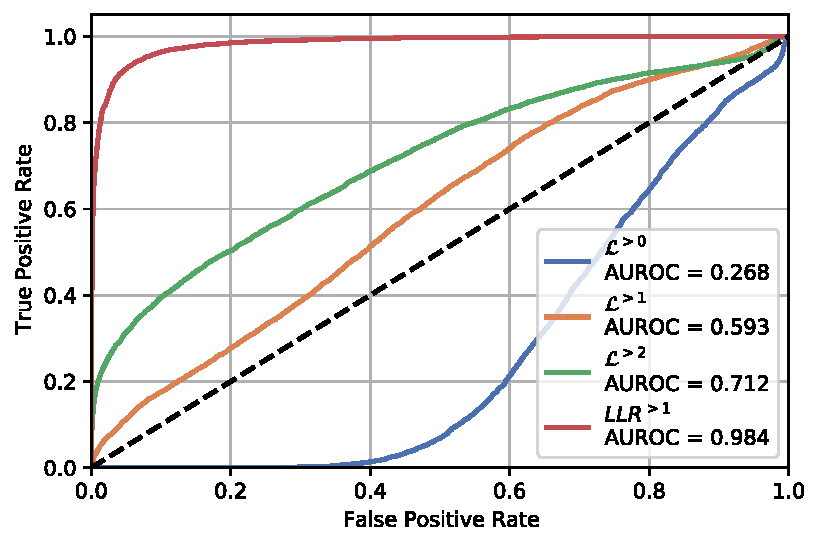
\includegraphics[width=1\columnwidth]{paper_hierarchical/roc-FashionMNIST-test-MNIST-test-ll-and-llr-IW250_sohau.pdf}
        \caption{}
        % \caption{ROC curves with AUROC score for detecting MNIST as OOD with the HVAE model trained on FashionMNIST.
        % A ROC curve is plotted for each of the $\mathcal{L}^{>k}$ bounds including the ELBO along with one for the best-performing log likelihood-ratio $LLR^{>1}$.}
        \label{fig_hierarchical:FMNIST-roc-llr}
    \end{subfigure}
    \hfill
    \begin{subfigure}[r]{0.495\columnwidth}
        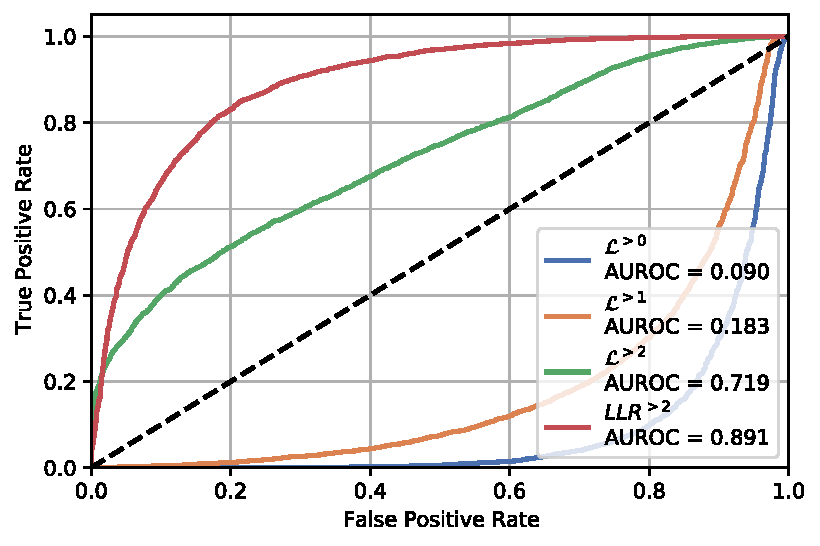
\includegraphics[width=1\columnwidth]{paper_hierarchical/roc-biva-CIFAR10-SVHN-ll-and-llr_sohau.pdf}
        \caption{}
        % \caption{ROC curves with AUROC score for detecting SVHN as OOD with the BIVA model trained on CIFAR10.
        % A ROC curve is plotted for each of the $\mathcal{L}^{>k}$ bounds including the ELBO along with one for the best-performing log likelihood-ratio $LLR^{>2}$.}
        \label{fig_hierarchical:CIFAR10-roc-llr}
    \end{subfigure}
    \caption[ROC curves for out of distribution detection (MNIST/FashionMNIST and SVHN/CIFAR10).]{%
        ROC curves with AUROC score for detecting \subref{fig_hierarchical:FMNIST-roc-llr} MNIST as OOD with the HVAE model trained on FashionMNIST and \subref{fig_hierarchical:CIFAR10-roc-llr} SVHN as OOD with the BIVA model trained on CIFAR10. 
        A ROC curve is plotted for each of the $\mathcal{L}^{>k}$ bounds including the ELBO along with one for the best-performing log likelihood-ratio $LLR^{>1}$.
    }
\end{figure}
We now move to the likelihood ratio-based score.
We find that $LLR^{>k}$ separates the OOD MNIST data from in-distribution FashionMNIST to a higher degree than the likelihood estimates as can be seen by the empirical densities of the score in \cref{fig_hierarchical:FMNIST-llr}.
We note that the likelihood ratio between the ELBO and the $\mathcal{L}^{>k}$ bound provides the highest degree of separation of MNIST and FashionMNIST as measured by the AUROC$\uparrow$ for $k=1$ smaller than $L$.
This is not surprising since the value of $k$ that provides the maximal separation to the reference in-distribution dataset need not be the one for which $\mathcal{LLR}^{>k}$ is overall maximal for the OOD dataset.
We also visualize the ROC curves resulting from using the $LLR^{>k}$ score for OOD detection on both FashionMNIST/MNIST and CIFAR10/SVHN and compare it to the ROC curves resulting from the different $\mathcal{L}^{>k}$ bounds in Figures \ref{fig_hierarchical:FMNIST-roc-llr} and \ref{fig_hierarchical:CIFAR10-roc-llr}, respectively.
On both datasets we see significantly better discriminatory performance when using the $LLR^{>k}$ score.

\cref{tab_hierarchical:rocauc-ood} shows that BIVA improves upon the HVAE model for OOD detection on CIFAR while \cref{tab_hierarchical:bits-per-dim-ood} shows that the BIVA model also improves upon the HVAE in terms of likelihood.
We hypothesize that models larger than our implementation of BIVA, with better likelihood scores may perform even better \cite{maaloe_biva_2019, vahdat_nvae_2020, child_very_2021}.


\subsection{Comparison to baselines}
\paragraph{Performance} \cref{tab_hierarchical:rocauc-ood} summarize our results compared to baselines based on the commonly used AUROC$\uparrow$, AUPRC$\uparrow$ and FPR80$\downarrow$ metrics.
Our method outperforms other generative model-based methods such as WAIC \cite{choi_waic_2019} with Glow model and performs similarly to the likelihood regret method of \cite{xiao_likelihood_2020}.
Furthermore, our method performs similarly to the background constrative likelihood ratio method of \textcite{ren_likelihood_2019} on FashionMNIST/MNIST but contrary to the failure of that method on CIFAR10/SVHN reported by \cite{xiao_likelihood_2020}, our method performs very well on this task too.
Our approach outperforms all supervised approaches that use in-distribution labels or synthetic examples of OOD data derived from the in-distribution data including ODIN \cite{liang_enhancing_2018} and the predictive distribution of a classifier $p(\hat{y}|\xb)$ trained and evaluated in various ways (see \textcite{ren_likelihood_2019}).

\paragraph{Runtime} For a full evaluation of a single example across all feature levels of a model with $L$ stochastic layers, our method requires $L-1$ forward passes through the inference and generative networks as well as computing the likelihood ratio, of which the forward passes are dominant.
For a typical forward pass that is linear in the input dimensionality, $D$, and the number of stochastic layers, $L$, this amounts to computation of $\mathcal{O}(DL)$.
Compared to some related work that either requires an $M>1$ sized batch of inputs of which either all or none are OOD \cite{nalisnick_detecting_2019} or cannot be applied to batches due to the required per-example optimization \cite{xiao_likelihood_2020}, our method additionally is applicable to batches of any size that may consist of both OOD and in-distribution examples which provides drastic speed-ups via vectorization and parallelization.
Furthermore, the method of \textcite{xiao_fashionmnist_2017} requires refitting the inference network of a VAE which can be computationally demanding.
Compared to the likelihood ratio proposed in \textcite{ren_likelihood_2019}, our method requires training only a single model on a single dataset.


\section{Discussion}
Deep generative models are state-of-the-art density estimators, but the OOD failures reported in recent years have raised concerns about the limitations of such density estimates. Recent work on improving OOD detection has largely sidestepped this concern by relying on additional assumptions that strictly should not be needed for models with explicit likelihoods.
While the engineering challenge of building reliable OOD detection schemes is important, it is of more fundamental importance to understand \emph{why} the naive likelihood test fails.
We have provided evidence that low-level features of the neural nets dominate the likelihood, which gives a \emph{cause} to the \emph{why}.
The fact that a simple score for measuring the importance of semantic features yield state-of-the-art results on OOD detection without access to additional information gives validity to our hypothesis.

The findings from, amongst others, \textcite{nalisnick_deep_2019, serra_input_2020} have a clear relation to information theory and compression. 
Semantically complex in-distribution data yields models with diverse low-level feature sets that enable generalization across datasets.
Simpler datasets can only yield models with less diverse low-level feature sets compared to complex training data.
Hence, there can be an asymmetry where the likelihoods of simple OOD data can be high for a model trained on complex data, but not the other way around.
Loosely put, the minimal number of bits required to losslessly compress data sampled from some distribution is the entropy of the generating process \cite{shannon_mathematical_1948, mackay_information_2003}.
\textcite{townsend_practical_2019} recently showed that VAEs can be used for lossless compression at rates superior to more generic algorithms.

We also note that since the hierarchical VAE is a probabilistic graphical latent variable model, it lends itself very naturally to manipulation at the feature level \cite{kingma_semi-supervised_2014, maaloe_auxiliary_2016, maaloe_semi-supervised_2017}.
This property sets it apart from other generative models that do not explicitly define such a hierarchy of features.
This in turn enables reliable OOD detection with our methodology while making no explicit assumptions about the nature of OOD data and only using a single model. This has not been achieved with autoregressive or flow-based models.

\section{Conclusion}
In this paper we study unsupervised out-of-distribution detection using hierarchical variational autoencoders.
We provide evidence that highly generalizeable low-level features contribute greatly to estimated likelihoods resulting in poor OOD detection performance.
We proceed to develop a likelihood-ratio based score for OOD detection and define it to explicitly ensure that data must be in-distribution across all feature levels to be regarded in-distribution.
This ratio is mathematically shown to perform OOD detection in the latent space of the model, removing the reliance on the troublesome input-space likelihood.
We point out that contrary to much recent literature on OOD detection, our approach is fully unsupervised and does not make assumptions about the nature of OOD data.
Finally, we demonstrate state-of-the-art performance on a wide range of OOD failure cases.


\section*{Acknowledgements}
This research was partially funded by the Innovation Fund Denmark via the Industrial PhD Programme (grant no.\@ 0153-00167B). JF and SH were funded in part by the Novo Nordisk Foundation (grant no.\@ NNF20OC0062606) via the Center for Basic Machine Learning Research in Life Science (MLLS, \hyperlink{https://www.mlls.dk}{https://www.mlls.dk}). JF was further funded by the Novo Nordisk Foundation (grant no.\@ NNF20OC0065611) and the Independent Research Fund Denmark (grant no.\@ 9131-00082B). SH was further funded by VILLUM FONDEN (15334) and the European Research Council (ERC) under the European Union’s Horizon 2020 research and innovation programme (grant agreement no. 757360).

% }
\part[supervised learning]{supervised learning}
\part[discussion and conclusions]{discussion and conclusions}
%!TEX root = ../thesis.tex

\chapter[discussion]{Discussion}\label{chp:discussion}
% ~5 pages
%
% OUTLINE:
% - paper-hierarchical:
%   - Suitability of VAEs for representation learning (minimization of mutual information and sensitivity to implicit prior such as architecture)
% - paper-benchmarking
%   - Inferiority of probabilistic methods compared to self"=supervised learning. 
% - 

The rapid progress of machine learning that started about a decade ago with the 2012 ImageNet competition and the work of \textcite{krizhevsky_imagenet_2012} all but slowed down during the course of this project. 
Following the papers by \textcite{choi_waic_2019,nalisnick_detecting_2019,hendrycks_deep_2019}, the field of out-of-distribution detection saw a surge of interest that has since grown yearly, while self"=supervised learning for speech has continued to advance with works such as CPC \parencite{oord_representation_2018}, wav2vec 2.0 \parencite{baevski_wav2vec_2020} and data2vec \parencite{baevski_data2vec_2022}. 

Having focused on VAEs for out-of-distribution detection in \cref{part:unsupervised-uncertainty-estimation} and on self"=supervised methods for representation learning in \cref{part:self-supervised-speech-representation-learning}, this discussion will bridge a gap between the two approaches and consider how VAEs might be enabled to learn representations more competitive with self"=supervised methods. 
Furthermore, since the work in \cref{part:medical-applications} only had limited focus on uncertainty, we will also present and discuss the use of calibration techniques for the stroke recognition model drawing connections to how such systems are perceived and used in practice. 


\section{Representation learning with variational autoencoders}
%
In this thesis we studied two different approaches to speech representation learning: VAEs in \cref{chp:paper-hierarchical,chp:paper-modelagnostic,chp:paper-benchmarking} and self"=supervised methods in \cref{chp:paper-review}. 
As we saw, the probabilistic formulation of VAEs provides benefits for their application to uncertainty quantification, although competitive methods that use self"=supervised foundation models have also been proposed \textcite{xiao_we_2021,hendrycks_using_2019,bergman_classificationbased_2020}. Self"=supervised methods are generally superior when it comes to performance on downstream tasks. While this of course depends on the task and the amount and type of unlabeled and labeled data, self"=supervised methods for speech are commonly evaluated on downstream tasks that are harder and more complex than those used for VAEs. For instance, between \cref{tab: phoneme recognition (PER),tab:unsupervisedASR} self"=supervised methods can be seen to outperform VAEs for phoneme recognition while self"=supervised methods are also reported for word-level speech recognition. 
In the following, we will discuss potential directions of future research that might help shed light on why VAEs representations underperform on downstream tasks and how they might be improved.


\paragraph{Designing the latent space} 
Architectural improvements and hierarchies of latent variables are two related, and interesting, approaches to learning more semantic features in VAEs. 
Some success has been demonstrated in the image domain with models like BIVA \parencite{maaloe_biva_2019}, NVAE \parencite{vahdat_nvae_2020}, and VD-VAE \parencite{child_very_2021}, with up to 78 stochastic layers, achieving tight likelihoods and high-quality samples, although limited effort has put towards using such models for downstream tasks. 
For speech, a hierarchical model operating on multiple temporal scales, such as the Clockwork VAE \parencite{saxena_clockwork_2021} adapted for speech in \cref{chp:paper-benchmarking}, might help better capture dependencies at longer ranges and encode more semantic features. 
For instance, phonetic content for pronunciation might be learned at lower layers, speaker identity at the upper layers, and semantic features, such as word-meaning, in between. 
Although some work has successfully separated speaker identity from content by modifying the latent variables and their dependencies \parencite{hsu_unsupervised_2017}, models that can learn a deep hierarchy of features for speech remains an open challenge. The work presented in \cref{chp:paper-benchmarking} represents an effort to make progress towards such a model. 


\paragraph{Adding a few labels} 
Another way to improve the representations learned in VAEs is via semi-supervised learning. 
Here, a few labels are used to inform which patterns that are learned from a large, mostly unlabeled, data set. 
This is usually done by defining a new stochastic variable as the target and deriving a semi-supervised version of the ELBO that accommodates using the labels when they are available, or marginalizing the target variable when they are not. The VAE is then trained on the labeled and unlabeled data simultaneously. 

Although VAEs are strong models for semi-supervised learning \parencite{kingma_semi-supervised_2014,kingma_improved_2016,maaloe_biva_2019}, self"=supervised methods have established themselves as superior for most tasks in this setting \cite{baevski_wav2vec_2020,jiang_speech_2021, liu_learning_2023}. 
Despite being theoretically appealing, joint objectives for semi-supervised learning in VAEs have practical drawbacks. By training on labeled and unlabeled data simultaneously, semi-supervised VAEs are often less flexible than are self"=supervised methods that divide the training into two separate phases. By first fitting a general foundation model in an expensive pre"=training phase it can then later be fine"=tuned for many downstream tasks, at relatively low cost. 
VAEs, on the other hand, must often learn the labeled downstream tasks while simultaneously training on the unlabeled data. This is computationally expensive, but also requires retraining with the unlabeled data, when new supervised data becomes available or a new task is added. 


\paragraph*{Approximating less}
VAE are inherently approximate. Training is performed on a lower bound of the likelihood and inference is variational, amortized and for non-hierarchical models, mean field. As a consequence, the gradient itself is estimated inexactly, usually by only one posterior sample, leading to non-negligible variance. 
For that reason, it seems plausible that using tighter bounds and reducing gradient variance improve representation learning in VAEs. 
Importance weighting the ELBO \parencite{burda_importance_2016} provides a tight bound on the likelihood, reduces gradient variance, and induces a complex implicit posterior distribution. 
Its use has become standard when reporting likelihood benchmarks but as we described in \cref{sec:variational-autoencoders}, \textcite{rainforth_tighter_2019} demonstrated that using it during training introduces high gradient variance for the inference network hurting its ability to learn useful representations. Later works largely solved this issue \parencite{roeder_sticking_2017,tucker_doubly_2019,bauer_generalized_2021} and showed that the reduced variance leads to improved likelihoods. 

Despite much of this progress being prior to the latest, very large hierarchical VAEs, such as BIVA \parencite{maaloe_biva_2019}, NVAE \parencite{vahdat_nvae_2020}, and VD-VAE \parencite{child_very_2021}, these models are all trained with the single-sample ELBO using regularly reparameterized gradient estimator. Instead, these models rely on advanced inference networks \parencite{maaloe_biva_2019} and architectural improvements \parencite{vahdat_nvae_2020, child_very_2021} to overcome the challenges of training hierarchical VAEs. 
This seems to indicate that there might be untapped potential in consolidating the work on low-variance gradient estimators and advanced architectures and inference networks.


\paragraph{Masking} 
As discussed in \cref{chp:paper-review}, masking is one of the driving techniques behind the success of self"=supervised methods for speech \parencite{devlin_bert_2018,baevski_wav2vec_2020}. By removing tokens from the input or an early feature extraction layer and tasking a model with inferring their representations, models are forced to learn how neighboring tokens relate to those masked. Depending on the size of the mask, these dependencies can be more or less semantic in nature. For instance, the wav2vec 2.0 model is well-known to learn representations that have high similarity with word identity and meaning \parencite{pasad_layerwise_2021}. 

In comparison, reconstruction in VAEs is done from latent variables that are inferred from the full, unmasked input. Since all information is generally available, this might allow the encoder and decoder models to perform well for reconstruction, even with no, or limited, use of contextual dependencies. Furthermore, VAE reconstruction almost always targets the direct input in order to learn the distribution over the training data and to enable generating new samples. However, compared to many self"=supervised methods that target intermediate, learned representations, this forces VAEs to encode all aspects of the input that are important to its distribution. As we saw in \cref{chp:paper-hierarchical}, this will generally include low-level features that are necessary for accurate input reconstruction. Such features require large latent space representations and model capacity \parencite{vahdat_nvae_2020,child_very_2021}, but are usually of lesser interest for downstream tasks \parencite{baevski_wav2vec_2020}.

Since the ELBO does not immediately allow for masking as part of the training, it has been only sparsely examined for VAEs. Specifically, masking has seen the most attention for VAEs within missing data imputation. In this setting, the input is partially observed, and often represented as a segmentation into observed and missing parts via a mask that indicates where the data is missing. The model is then trained to infer the latent variable from the observed data and reconstruction also deals only with the observed data. 
By comparison to self"=supervised approaches that use masking for representation learning, the missing data setting of VAEs focuses on reconstructing the observed data rather than the missing, which might not lead to the same benefits in representation learning. 

The idea of using VAEs to impute missing data was already examined in the seminal paper by \textcite{rezende_stochastic_2014}. Here the model was trained with fully observed data and used to impute data in an iterative sampling approach post hoc, leaving the learned representations unchanged.
Previous work that trains on partially observed data has largely focused on the ability of these models to yield high-quality imputations within the tabular and image data domains and have not probed for the effects on the learned latent representation \parencite{mattei_miwae_2019, ipsen_not-miwae_2021}. 

Including masked objectives into the principled probabilistic framework of VAEs might require creative thinking, but it seems likely that relaxing the requirement of exact input reconstruction and enforcing the need of encoding (and decoding) contextual information could lead the way for future types of VAEs to learn representations that are competitive with self"=supervised methods.


\paragraph{Giving up?}



\parencite{tomczak_trouble_2022}
\parencite{huszar_is_2017}

\lesstodo[inline]{Discuss whether VAEs are even suitable for representation learning due to them minimizing a mutual information term in the ELBO (derive this form).}
\lesstodo[inline]{Discuss sensitivity to ``implicit" prior such as architecture (and probably optimization method and other). Include reference to \parencite{huszar_is_2017} discussing the usefulness of using a maximum likelihood objective for representation learning in generative models.}




\lesstodo[inline]{Out-of-distribution detection on speech?}






% \subsection{Uncertainty estimation with self-supervised methods}
% %

% \textcite{pasad_layerwise_2021} found that layers 6-7 hold the most information about phonetic content and word identity and meaning for \texttt{wav2vec2-base}. 
% For \texttt{wav2vec2-large} the phonetic content is highest in layers 11 and 18-19 with a drop in between, while word identity and meaning are highest between layers 12 and 18. 


% Uncertainty of representations versus uncertainty of downstream task outputs. 
% % \textcite{wickstrom_relax_2023} propose a method for quantifying uncertainty based on 




% \section{\Cref{chp:paper-review} revisited: \dots} \label{sec:discussion-paper-review}

% \lesstodo[inline]{Are self"=supervised speech representations useful for unsupervised uncertainty estimation? \parencite{nava_stateconsistency_2021, nava_uncertaintyaware_2021} Within robotics but not really related.}
% % Since the main focus within self"=supervised learning has been on improving downstream task performance, very limited work, if any, has investigated self"=supervised representations in terms of uncertainty estimation. 
% % However, in the context of medical applications where data can be abundant but labels are sparse, unsupervised uncertainty estimation is a very interesting direction for future work.
% \lesstodo[inline]{OOD data: Generalization or detection (https://arxiv.org/pdf/2110.11334.pdf)?}




\section{\Cref{chp:paper-retrospective} revisited: Calibration}

\begin{figure}
    \centering
    \begin{subfigure}[c]{0.49\columnwidth}
        \centering
        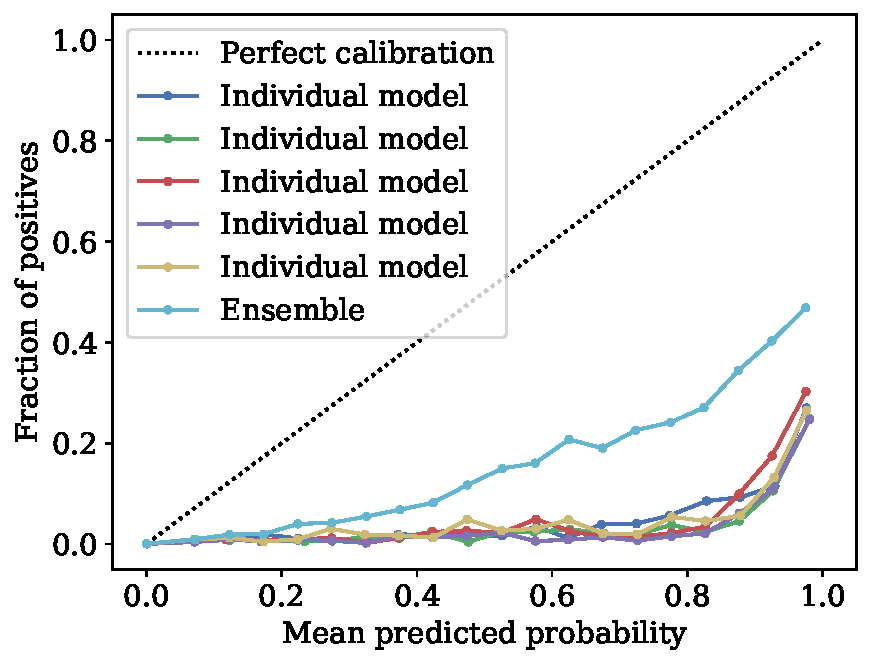
\includegraphics[width=1\columnwidth]{paper_retrospective_calibration_plots/calibration_curve_ensemble_and_all_models_uncalibrated.pdf}
        % \caption{}
        % \label{fig_discussion:calibration_curve_ensemble_and_all_models_uncalibrated}
    \end{subfigure}
    \hfill
    \begin{subfigure}[c]{0.49\columnwidth}
        \centering
        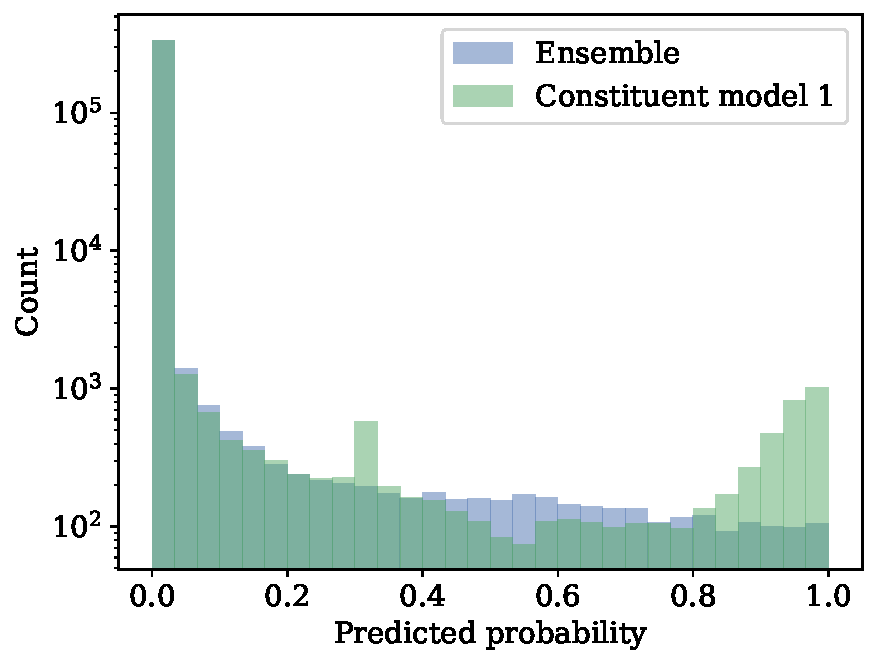
\includegraphics[width=1\columnwidth]{paper_retrospective_calibration_plots/histogram_ensemble_and_single_model.pdf}
        % \caption{}
        % \label{fig_discussion:histogram_ensemble_and_single_model}
    \end{subfigure}
    \caption[Calibration curve for the uncalibrated stroke recognition ensemble and empirical distribution of predicted probabilities.]{ Calibration curve for the uncalibrated stroke recognition ensemble (left) and the histogram of predicted probabilities (right) for the test set. We use the ensemble that achieved the median F1-score reported in \cref{fig_retrospective:figure1-roc-curve} and \cref{tab_retrospective:table3-occlusion-analysis}.}
    \label{fig_discussion:retrospective-paper-calibration-curve-of-uncalibrated-model}
\end{figure}

Our work on stroke recognition in \cref{chp:paper-retrospective} focuses on the predictive performance of the ensemble model and an analysis of feature importance, but does not explicitly consider uncertainty estimation. 
As we discussed in \cref{subsec:model-calibration}, such a model can be calibrated to predict probabilities that are aligned with the empirical probability of the model being correct on some validation set. Here we present and discuss model calibration for the ensemble model. 

We compute the calibration curve by sorting the probabilities predicted on the test set into a number of bins spanning the range from zero to one. For each bin $b$, we compute the mean predicted probability $\bar{p}$ and the fraction of examples for which the model predicted correctly $r_{b}$. The calibration curve is the drawn from the $\{(\bar{p}_{b}, r_{b})\}_b$ pairs. For any given bin, a perfectly calibrated model would have the same fraction of correct predictions as that bin's mean value, $\bar{p}_{b} = r_{b}\,\forall\,b$. 

The calibration curve for the uncalibrated stroke recognition ensemble and its constituent models is plotted in \cref{fig_discussion:retrospective-paper-calibration-curve-of-uncalibrated-model} along with a histogram of its predicted probabilities. The miscalibration issue that we previously discussed is clearly visible as a strong overconfidence for both ensemble and constituents, although the ensemble is much better calibrated than its constituents. Since the ensemble's output probability is computed as the harmonic mean of the five constituent model probabilities, it can never exceed the maximum probability predicted between the constituent models. This property tends to make ensemble probabilities less extreme and, since the constituent models are overconfident, this results in better calibration (see also the histogram in \cref{fig_discussion:retrospective-paper-calibration-curve-of-uncalibrated-model}). 

\begin{figure}
    \centering
    \begin{subfigure}[c]{0.49\columnwidth}
        \centering
        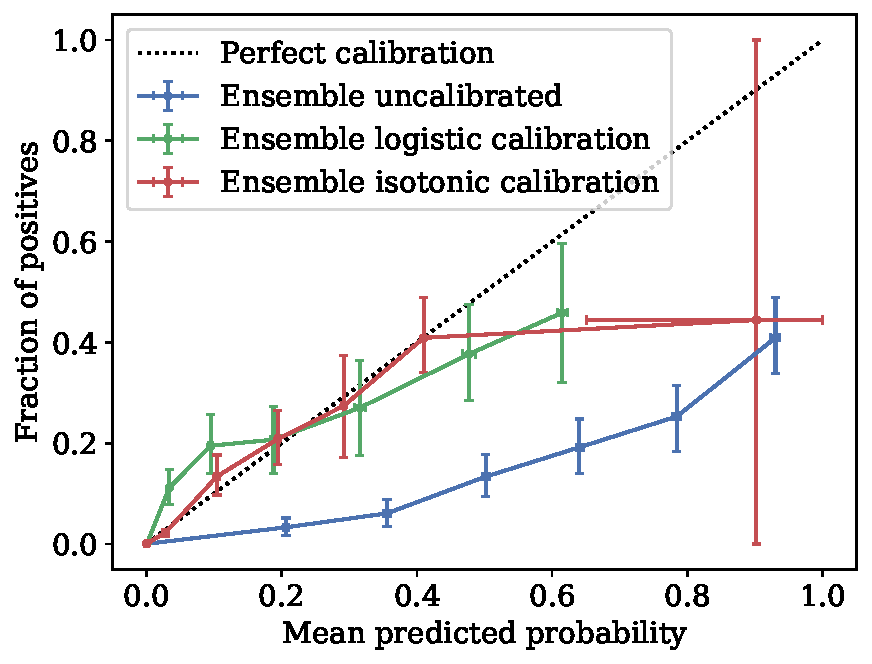
\includegraphics[width=1\columnwidth]{paper_retrospective_calibration_plots/calibration_curves_ensemble_with_cis.pdf}
    \end{subfigure}
    \hfill
    \begin{subfigure}[c]{0.49\columnwidth}
        \centering
        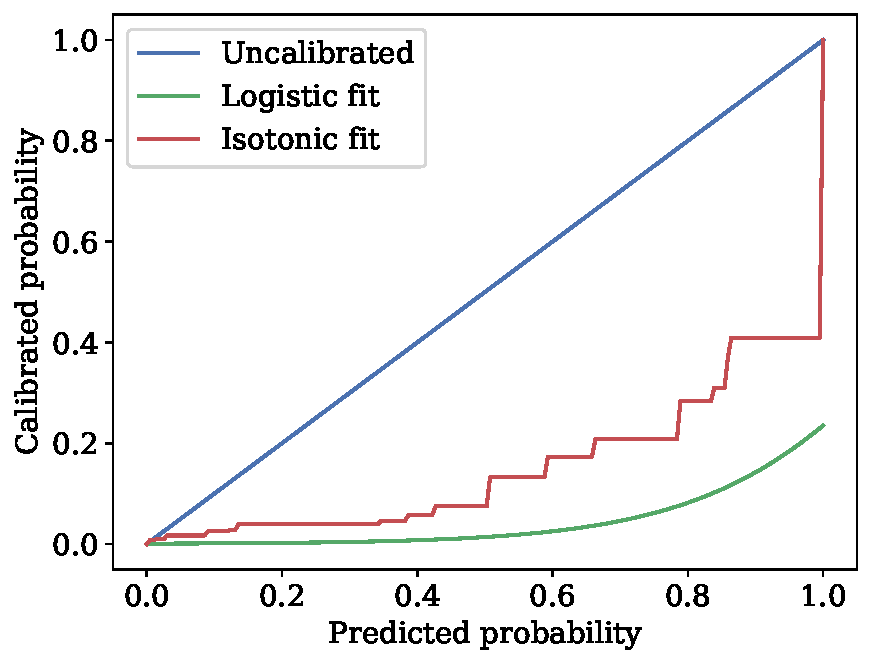
\includegraphics[width=1\columnwidth]{paper_retrospective_calibration_plots/calibration_fits_ensemble.pdf}
    \end{subfigure}    
    \caption[Calibration fits and curves for the stroke recognition ensemble using Platt-scaling and isotonic regression for calibration.]{ Calibration curves using sigmoid and isotonic calibration fits for the stroke recognition ensemble model (left) and the calibration fits (right) for the test set. We use the ensemble that achieved the median F1-score reported in \cref{fig_retrospective:figure1-roc-curve} and \cref{tab_retrospective:table3-occlusion-analysis}.}
    \label{fig_discussion:retrospective-paper-calibration-curve-sigmoid-isotonic}
\end{figure}

To calibrate the ensemble model, we can use methods such as Platt-scaling \parencite{platt_probabilistic_1999} or isotonic regression \parencite{zadrozny_transforming_2002}. 
In either case, we fit a simple regression model (logistic or isotonic) to the predicted probabilities and the target labels on the validation set and use it to adjust the probabilities predicted on the test set. We show the resulting calibration curves on the left in \cref{fig_discussion:retrospective-paper-calibration-curve-sigmoid-isotonic} and the logistic and isotonic fits on the right with 95\% bootstrap confidence intervals on the bin centers ($x$ error) and fraction of positives ($y$ error). 
% In \cref{fig_discussion:retrospective-paper-calibration-curve-sigmoid-isotonic} we have done so for the ensemble model and visualize the results on the test set. 
% On the left, we plot the resulting calibration curves and on the right we show the logistic and isotonic fits. 
We see that both methods result in quite good calibrations\footnote{Brier scores on test set: Uncalibrated = $0.003500$, logistic = $0.001807$, isotonic = $0.001774$. Relative improvement in Brier score compared to uncalibrated (Brier skill score): Logistic = $0.4830$, isotonic = $0.4924$.} and that the predicted probabilities are shifted towards smaller values. 
Since stroke cases have low prevalence, high probability is predicted only for a few examples (see histogram in \cref{fig_discussion:retrospective-paper-calibration-curve-of-uncalibrated-model}). This leads to a lack of data for the calibration fits at high predicted probabilities which can be seen to result in poor generalization to the test set, especially for the nonparametric isotonic regression.

% Brier scores:  {'uncalibrated': 0.0034955788687128925, 'logistic': 0.0018072483306197486, 'isotonic': 0.0017744177396100578, 'average': 0.0021955477869598783}
% BSS uncalibrated reference:  {'logistic': 0.48299025755205005, 'isotonic': 0.4923822902432705}
% BSS mean reference:  {'logistic': 0.17685766561145932, 'isotonic': 0.1918109229282361}

\begin{figure}
    \centering
    \begin{subfigure}[c]{0.49\columnwidth}
        \centering
        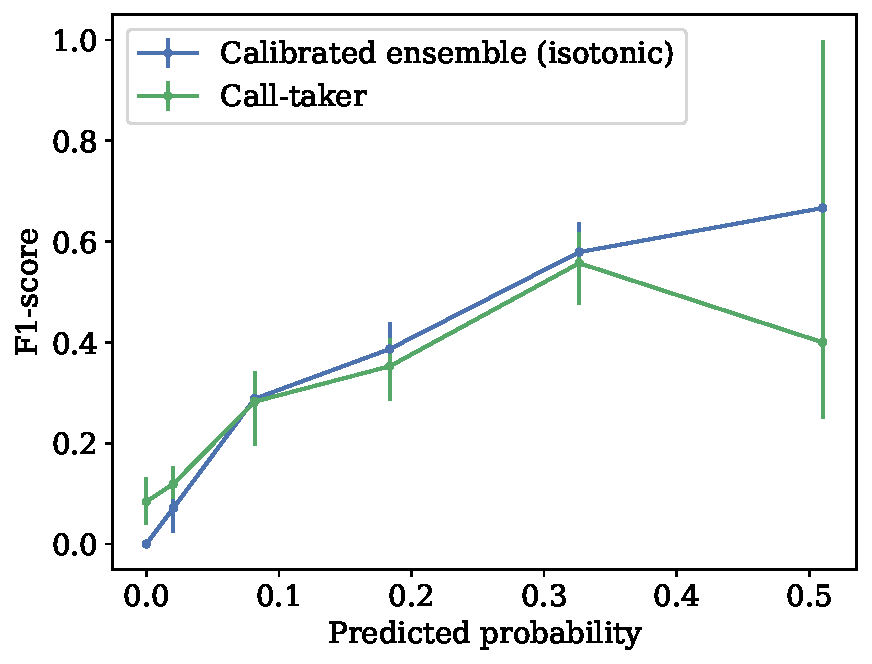
\includegraphics[width=1\columnwidth]{paper_retrospective_calibration_plots/f1_score_vs_predicted_probability_ensemble_calltaker_with_cis.pdf}
    \end{subfigure}
    \hfill
    \begin{subfigure}[c]{0.49\columnwidth}
        \centering
        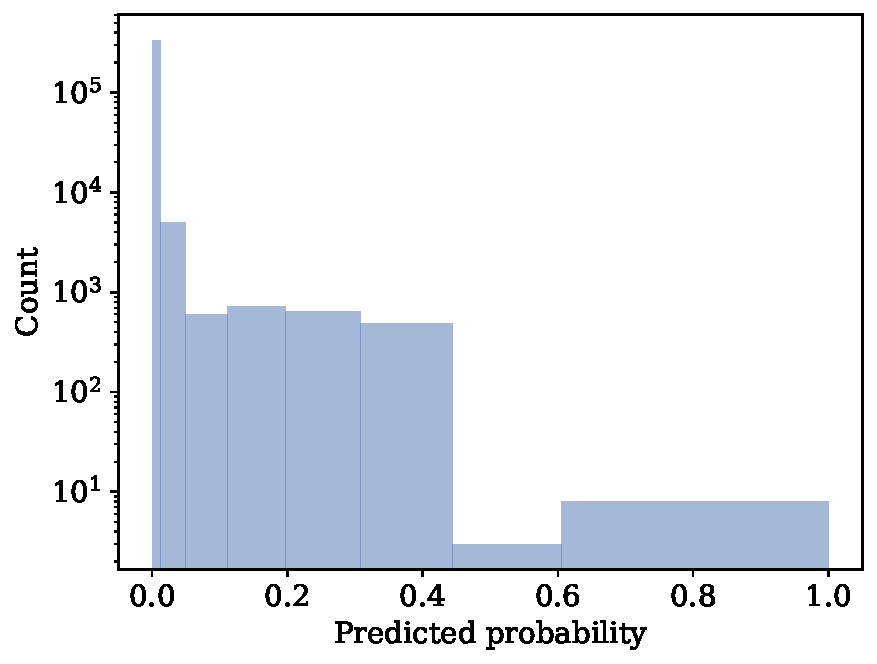
\includegraphics[width=1\columnwidth]{paper_retrospective_calibration_plots/predicted_probability_histogram.pdf}
    \end{subfigure}    
    \caption[Comparison of F1-score of stroke recognition ensemble and call-takers as function of predicted probability.]{ Comparison of the F1-score of the stroke recognition ensemble and call-takers. The F1-score is computed on subsets of the test dataset made by binning on the predicted probabilities of the calibrated ensemble. We see that the relative performance improvement of the ensemble over call-takers is higher towards more certain predictions. We use the ensemble that achieved the median F1-score reported in \cref{fig_retrospective:figure1-roc-curve} and \cref{tab_retrospective:table3-occlusion-analysis}.}
    \label{fig_discussion:retrospective-paper-f1-performance-vs-predicted-probability}
    % \begin{subfigure}[c]{0.49\columnwidth}
    %     \centering
    %     \includegraphics[width=1\columnwidth]{paper_retrospective_calibration_plots/precision_vs_predicted_probability_ensemble_calltaker_with_cis.pdf}
    %     % \caption{}
    %     % \label{fig_discussion:calibration_curve_ensemble_and_all_models_uncalibrated}
    % \end{subfigure}    
    % % \hfill
    % \begin{subfigure}[c]{0.49\columnwidth}
    %     \centering
    %     \includegraphics[width=1\columnwidth]{paper_retrospective_calibration_plots/recall_vs_predicted_probability_ensemble_calltaker_with_cis.pdf}
    %     % \caption{}
    %     % \label{fig_discussion:histogram_ensemble_and_single_model}
    % \end{subfigure}
\end{figure}

Clinicians in intensive care units and emergency departments have been found to strongly agree that a singular focus on overall accuracy cannot alone ensure sustained trust in a model \cite{tonekaboni_what_2019}. Clinicians expect an alert to present a prediction that aligns with patient status. Despite expert-agreed thresholds for when alerts should be triggered, however, many alerts may not be aligned since class imbalance and ambiguous information in many predictive problems in healthcare can lead to models with relatively low predictive precision \parencite{umscheid_development_2015, cite14, cite15, wenstrup_retrospective_2023}. In turn, this is likely to lead to alarm fatigue \parencite{embi_evaluating_2012} and can undermine the sustained use and endorsement by clinicians of such systems \parencite{guidi_clinician_2015}. 
The stroke recognition ensemble presented in \cref{chp:paper-retrospective} is not exempt from this risk. With a precision of $24.9\%$ (95\% confidence interval $24.3-25.5\%$) it will on average be wrong three out of four times it predicts a stroke. This unfortunately risks alarm fatigue among its potential users diminishing its effect in practice.

% If the stroke recognition ensemble were to be deployed in a randomized controlled trial, s
Calibrated probabilities in the alerts presented to users might be a way to alleviate alarm fatigue. Calibrated probabilities would allow users to discern between certain and uncertain predictions and also enable the system to present users only with predictions that have at least a certain probability of being correct. Similar approaches have been suggested by clinicians and interviews indicate that predictive uncertainty is perceived by experts as a sort of explanation that complements the prediction \cite{tonekaboni_what_2019}. In \cref{fig_discussion:retrospective-paper-f1-performance-vs-predicted-probability} we show the F1-score of the ensemble model and the call-takers computed on subsets of the data created by binning the calibrated probabilities. We note that, as might be expected, both call-taker and ensemble model performance increase with increased model certainty. This indicates that selecting, based on certainty, which predictions to present to users might indeed help build trust in the system and ensure a practical impact. 


% \lesstodo[inline]{Maybe mention MultiQT paper \parencite{havtorn_multiqt_2020}.}

%!TEX root = ../thesis.tex

\chapter[conclusions and outlook]{Conclusions and outlook}\label{chp:conclusion}
% ~3 pages

\textbf{\Cref{chp:introduction}} introduced the motivational cases of automated medical coding and stroke recognition and used them to exemplify the importance of out"=of"=distribution detection, and, by extension, representation learning. In the context of these cases, we discussed possible machine learning system designs for decision support and considered potential sources of uncertainty and ideal model behavior. 
The cases form a reference point for the thesis as a whole, connecting its contributions within out"=of"=distribution detection and representation learning back to practical applications. 
In this conclusion, we will review the studies presented in previous chapters in the context of the discussion of \cref{chp:discussion} and the recent progress in the field, and point to interesting directions of future research. 
As \textbf{\cref{chp:main-contributions}} already details the contributions made by this thesis, we will not reiterate them in detail in this conclusion. 

% \textbf{\cref{chp:introduction}} laid out how progress-driving technological development has always come with new challenges and risks of error - whether via misuse, misunderstanding or inherent limitations. We emphasized that machine learning comes with these same types of risk, in some cases amplifying their impacts, and argued that uncertainty estimation is a key component in ensuring that systems are safe and reliable in practice. 

% The chapter also provided some background for the research project by introducing the health tech company Corti, with which with project has been defined and carried out, and the motivational cases of recognition of stroke cases in emergency calls (\cref{subsec:motivation-stroke-recognition}) and automated medical coding (\cref{subsec:motivation-medical-coding}). Using these cases, we exemplified how uncertainty might arise in practice and how quantifying it might improve the usefulness of machine learning systems built for the tasks.
% Finally, we drew connections between machine learning reliability (\cref{sec:machine-learning-reliability}) and model calibration (\cref{subsec:model-calibration}) and defined the aleatoric, epistemic, and predictive types of uncertainty (\cref{subsec:understanding-uncertainty}). 

% Along with the technical background provided in
% This introduction formed the basis of 


\vspace{1em}
\textbf{\Cref{chp:technical-background}} provided in-depth technical background that could only be covered briefly by the individual studies. 
We first introduced uncertainty as a concept in the context of information and probability theory (\cref{sec:uncertainty-information-theory}). We then defined the task of out-of-distribution detection and reviewed existing work on the problem (\cref{sec:out-of-distribution-detection}). Finally, we provided technical background for variational autoencoders (\cref{sec:variational-autoencoders}).

\vspace{1em}
\textbf{\Cref{chp:paper-hierarchical}} showed how hierarchical variational autoencoders can fail at likelihood"-based OOD detection due to an overemphasis on low-level features that generalize between different data distributions. 
In other words, the latent representations of high-dimensional data from different distributions overlap, especially for latent variables low in the hierarchy.
By exploiting that VAEs tend to learn more abstract features at latent variables high in the hierarchy, we were able to define a likelihood-ratio score that focused more on features unlikely to be shared between datasets and performed much better for OOD detection. 
In line with our discussion in \cref{sec_discussion:representation-learning-with-vaes}, these findings show that VAEs can indeed learn useful latent representations, although good performance, at least for OOD detection, might require selecting an appropriate subset of latent representations to use. 
Similar variations among features learned at different layers have also been identified for self"=supervised models and speech representations \parencite{pasad_layerwise_2021}. 
To obtain good downstream task performance, this suggests that, besides seeking to improve representations overall, future research effort should also be directed towards finding good methods for selecting relevant subsets of latent variables in a given hierarchical VAE for a certain task.
% - VAEs can learn useful representations, but it can be hard to impose the appropriate constraints that enable this.
% - VAEs can learn representations that are useful for OOD detection, but good performance might require selecting an appropriate subset of feature dimensions to use for discriminating.
% Our work shows that a promising direction of future research is into how to select which dimensions are the most discriminatory.

% In this work we hypothesize that the likelihood estimate of variational autoencoders is a poor score for out-of-distribution due to an overemphasis on low-level features that generalize between distributions. 
% We further hypothesize that a well-formed hierarchy of latent variables provides a tool that can be used to select which features to emphasize for out-of-distribution detection and, hence, a way to improve the performance of variational autoencoders on this task. 
% We proceed to provide empirical and theoretical evidence that low-level features do indeed dominate the likelihood score and propose a new method for out-of-distribution detection using hierarchical variational autoencoders based on a likelihood-ratio score that requires data to be in-distribution across all feature-levels. 
% The proposed method is computationally efficient, fully unsupervised, and performs well on several out-of-distribution detection benchmarks. 

\vspace{1em}
\textbf{\Cref{chp:paper-modelagnostic}} took a different approach to OOD detection than \cref{chp:paper-hierarchical} and focused on developing a model-agnostic method. 
We showed that by phrasing OOD detection as a statistical testing problem and combining different tests, orthogonal properties of the individual tests could be leveraged to improve the OOD detection performance over any single test.
%
The formulation of OOD detection as a statistical test also allows for better guarantees for such systems in practice. For instance, as also discussed in \cref{chp:paper-modelagnostic}, the statistical framework enables false positive rate control which is a valuable property in many practical applications especially if they involve high-risk actions such as in medical decision support. 


% In this follow-up work to \cref{chp:paper-hierarchical}, we note that the set of methods proposed for out-of-distribution detection using generative models is quite large and that many are tailored for specific model types, which suggests that it is possible to develop a model-agnostic approach. We hypothesize that by phrasing the task as a statistical testing problem and combining different tests, the method's efficacy can be improved and weaknesses inherent to any particular test can be alleviated. 
% From this hypothesis, we combine a classical parametric test with the recently introduced typicality test to develop a method applicable to any differentiable  generative model with explicit likelihood, and show that this leads to a more accurate out-of-distribution test. 
% Finally, we discuss the benefits of casting out-of-distribution detection as a statistical testing problem, for instance enabling false positive rate control. This property is valuable in many practical applications, especially in high-risk settings such as medical decision-making.



\vspace{1em}
\textbf{\Cref{chp:paper-brief}} provided an overview of unsupervised neural speech representation learning. Such approaches have recently matched supervised methods on many tasks and represent a significant advance in low-resource settings, such as speech recognition for minority languages. 
We found that for the purpose of learning good representations in an unsupervised manner, self-supervised learning seems to have better inductive biases, or at least pose a more forgiving learning problem, than do VAEs. As discussed in \cref{chp:paper-brief,sec_discussion:representation-learning-with-vaes}, this likely relates more to inductive biases imposed by implicit constraints in the optimization problem and architecture than to the underlying formalism. 
For instance, in discussion about the weaknesses of VAE-based approaches (\cref{sec_discussion:representation-learning-with-vaes}) we concluded that their challenges could not be directly attributed to the maximum marginal likelihood objective. Indeed, the masked pre-training objective widely used for successful self"=supervised methods has also been identified to correspond to a maximum marginal likelihood objective \parencite{moreno-munoz_masked_2023}. 

This also leaves potential for future work to improve the ability of VAEs to learn useful representations. As discussed in \cref{chp:paper-brief,sec_discussion:representation-learning-with-vaes}, promising approaches include adopting masked objectives for VAE training, improving architectural designs to impose better inductive biases, and incorporating advances in gradient estimators more widely \parencite{rainforth_tighter_2019,roeder_sticking_2017,tucker_doubly_2019,bauer_generalized_2021}, especially works on large VAE models \parencite{maaloe_biva_2019,vahdat_nvae_2020,child_very_2021}. 

% As we discussed in \cref{chp:discussion}, there are many interesting avenues of future research for improving the ability of VAEs to learn useful representations, including better gradient estimates and masked objectives.

% In this chapter, we present a comprehensive overview of unsupervised neural representation learning for speech. Previous research is categorized into self"-supervised methods and probabilistic latent variable models and described in a common notation. This description assists in developing a model taxonomy that shapes a discussion of the models' representational power, the associated learning strategies, and the methods used to evaluate them. The discussion points to interesting avenues of future research. 

% Chapter 6 presented an overview of unsupervised neural speech representation learning. As emphasized in the overview, the wav2vec 2.0 framework [13], and masked pre-training in general, represent a breakthrough in low-resource speech recognition. The challenge associated with obtaining training data for conversational speech recognition, as discussed in section 1.2.1, has become much smaller. Even when no labeled in-domain data is available, this framework offers a viable solution [112].

% The general idea for masked pre-training may seem simple; reconstruct masked parts of the input or another representation, given context. However, this methodology aligns very well with the general definition of semantics presented in section 1.4: "semantic properties of a lexical item are fully reflected in appropriate aspects of the relations it contracts with actual and potential contexts" ([63], p. 1). Thus, from a philosophical point-of-view, it may be difficult to see how the field should move on from here. Of course, context is more than just the neighboring words in a speech segment. The next wave of representation learning for speech incorporates multiple modalities, such as video [244, 245] or text [18]. Furthermore, how to construct targets for pre-training these models and how that affects the learned features is an avenue that warrants more research. This is of particular interest in the speech domain, where the input codes for speaker identity and emotional state, as well as the semantic content of the utterance.

\vspace{1em}
\textbf{\Cref{chp:paper-benchmarking}} conducted a comprehensive evaluation of stochastic and deterministic generative models, focusing on their model likelihood. 
The chapter also introduced a novel hierarchical VAE type model for speech, by drawing inspiration from the Clockwork VAE \parencite{saxena_clockwork_2021}. 
Despite the limitations of VAEs for representation learning as compared to self"=supervised methods (\cref{chp:discussion}), for sequence data, hierarchical VAE models that operate on multiple temporal scales provide a natural framework for encoding distinct feature categories. 
For instance, pronunciation features might be learned at lower layers, speaker identity at upper layers, and semantic features in intermediate layers. Despite successful attempts at isolating speaker identity from content in some existing work \parencite{hsu_unsupervised_2017}, developing VAE models with the capacity to learn a deep hierarchy of features for speech persists. The model presented in \cref{chp:paper-benchmarking} is an attempt at this challenge.
% Despite the current limitations, VAEs possess a unique ability to learn a distribution over the training data, requiring them to encode diverse aspects of the dataset. This inclusivity, while potentially redundant for certain tasks, proves advantageous for others that benefit from a wide array of features. 

\vspace{1em}
\textbf{\Cref{chp:paper-automated}} examined existing works on automated medical coding and found that in many cases training was suboptimal and evaluation standards were biased. We performed a revised comparison of the selected models and provided updated conclusions on the relative performance of models, and the impact of rare codes and long discharge note documents. 

The practical impact of the work of \cref{chp:paper-automated}, and the work in the field of medical coding in general, depend on a number of factors. 
Much of the field has focused on the MIMIC datasets which originate from the emergency department and ICU of a single hospital. These datasets have enabled much of the progress in the field, but their singular data source also reduces the generality of the derived results and risks biasing the directions of research deemed most impactful \parencite{tengReviewDeepNeural2022, venkateshAutomatingOverburdenedClinical2023,johnsonMIMICIIIFreelyAccessible2016,johnsonMIMICIVFreelyAccessible2023}. 
Furthermore, the complexity and multi-label nature of medical coding has lead to a high prevalence of label errors in MIMIC-III \parencite{searleExperimentalEvaluationDevelopment2020}. While difficult to remove entirely, having multiple diverse datasets would also alleviate the risk that the biases of such errors lead to misguided conclusions. Besides gathering more data, improved evaluation methods, such as human-in-the-loop, could be useful to increase the reliability of results. 

A common weakness of medical coding models is that performance varies widely between classes. The long-tailed distribution of code-frequency is particularly challenging and leads to underperformance on rare codes. Practical applications could still benefit from such models though. By limiting model predictions to a subset of codes for which they perform well, practitioners could focus on harder to code cases. This selection of cases in practical applications of medical coding could also benefit from research into selective prediction \parencite{geifman_selective_2017}. 
Although pre"=training is an obvious approach to improve performance when little data is available, compared to the effect of pre"=training in other domains \parencite{mohamed_selfsupervised_2022, linPretrainedTransformersText2021,baevski_wav2vec_2020,devlin_bert_2018,dosovitskiy_image_2021}, the improvements observed by using pre"=trained models for medical coding have been limited \parencite{jiDoesMagicBERT2021,gaoLimitationsTransformersClinical2021,michalopoulosICDBigBirdContextualEmbedding2022,pascualBERTbasedAutomaticICD2021,zhangBERTXMLLargeScale2020}. This suggests an untapped potential for future research into more targeted pre"=training for medical coding. 

While our work in \cref{chp:paper-automated} focused on unimodal medical coding models, it is highly likely that future state-of-the-art models will augment discharge summaries with multi-modal inputs such as medical code descriptions, synonyms, and hierarchies \parencite{kimReadAttendCode2021, mullenbachExplainablePredictionMedical2018, vuLabelAttentionModel2020, caoHyperCoreHyperbolicCograph2020, baoMedicalCodePrediction2021, yuanCodeSynonymsMatter2022,caoHyperCoreHyperbolicCograph2020, xieEHRCodingMultiscale2019}. 
This is particularly useful since coding standards are updated regularly. 
The ICD standard for instance sees revisions and new codes added yearly, with local adoption following national guidelines \parencite{centerfordiseasecontrolandpreventioncdc_international_2023}. 
Leveraging such modalities will enable adapting models to updated coding standards without having to gather large amounts of new data. 


% The use of supportive systems for medical coding in practice relies on 

% - Errors in the gold-standard data: \textcite{searleExperimentalEvaluationDevelopment2020} investigated the quality of the human annotations in MIMIC-III and concluded that 35\% of the common codes were under-coded. Such errors and subjectivity in manual medical coding make model training and evaluation challenging and suggests that additional evaluation methods using, e.g., a human-in-the-loop, could be useful to increase the reliability of results. 

% Future directions
% - Avoiding predicting several mutually exclusive classes, which is a general problem for multi-label classification.

% - research should focus on improving performance on rare codes while, in the shorter term, developing methods to detect codes that are too challenging for automated coding and, therefore, should be coded manually

% - Fully leveraging pre"=training (while PLM-ICD outperforms the other models in this paper, the improvements are limited compared to the effect of pre"=training in other domains \parencite{mohamed_selfsupervised_2022, linPretrainedTransformersText2021,baevski_wav2vec_2020,devlin_bert_2018,dosovitskiy_image_2021}) 
% Notably, there have been several unsuccessful attempts at using pre"=trained transformers for medical coding \parencite{jiDoesMagicBERT2021,gaoLimitationsTransformersClinical2021,michalopoulosICDBigBirdContextualEmbedding2022,pascualBERTbasedAutomaticICD2021,zhangBERTXMLLargeScale2020}

% - Generalization to other hospitals. discharge summaries from outpatient care are often easier to code than summaries from inpatient care as they are shorter with fewer codes per document \parencite{zhangBERTXMLLargeScale2020, liuEffectiveConvolutionalAttention2021, tsengAdministrativeCostsAssociated2018}





\vspace{1em}
\textbf{\Cref{chp:paper-retrospective}} studied how machine learning might be used to improve decision-making at emergency services in relation to stroke detection. 
We saw that a model was able to improve significantly on the stroke recognition ability of call-takers alone and that the features it used were sensible and related to symptoms and descriptions of stroke. 

In \cref{sec: discussion-stroke-recognition-uncertainty}, we discussed how calibrating the predictive uncertainty of the stroke model is likely to be necessary to ensure sustained use of such a model in practice. In \cref{fig_discussion:retrospective-paper-f1-performance-vs-predicted-probability}, we noted that, as expected, model performance measured by F1-score increased with increasing model certainty which underlines the likely usefulness of uncertainty estimates in better matching practitioner expectations of the predictive performance. 
Nonetheless, basic metrics of model performance might still be obstacles for its practical usefulness. Specifically, the rarity of stroke cases lead to relatively high false positive rate and low precision, likely to induce alarm fatigue among its users. Similar effects are likely to have influenced the practical impact of a similar system for cardiac arrest detection which also showed significant improvements in a retrospective study \parencite{cite14}. Although the model later matched the retrospective results in a prospective study, it did not ultimately result in improved call-taker performance \parencite{cite15}. 

Nevertheless, the strong retrospective performance of the stroke recognition model indicates that there is significant potential for augmenting the medical interview to allow better recognizing stroke cases. 
Possible improvements to the system could include using the audio signal to detect speech-related symptoms such mumbling or slurring, or integrating with electronic health-records to cross-reference with patient history. 
Even so, directly predicting the diagnosis from the conversation is not the only path towards practical impact. By suggesting informative questions to the medical professional, a system could also help guide the course of conversation to avoid missing important details and keep an overview, and to in turn improve the performance of the model. 
Ultimately, machine learning has proven capable of contributing meaningfully to medical conversations aiming to improve patient outcomes. Future work seems poised to make a significant positive impact on the healthcare industry over the years to come. 


% Explore the utilization of audio data 
% in conjunction with EHR information to gain a comprehensive understanding of the patient's condition.


% Suggesting Questions:

% Integrate the ML system into the interview framework to dynamically suggest relevant questions based on the ongoing conversation. This approach leverages the model's retrospective success, guiding clinicians to inquire about specific symptoms or risk factors that may contribute to more accurate stroke identification.

% Fact/Sanity-Checking with Electronic Health Record (EHR):

% Establish a seamless connection between the ML model and the patient's EHR to perform real-time fact-checking during the interview. This ensures the accuracy of the information provided by the patient, enhancing the reliability of the diagnostic process.

% Improved Understanding of the Patient Using Audio and EHR:

% Explore the utilization of audio data in conjunction with EHR information to gain a comprehensive understanding of the patient's condition. By analyzing speech patterns, tone, and content, the ML model can contribute valuable insights to the diagnostic process. Additionally, cross-referencing this audio data with EHR details enhances the model's ability to discern subtle indicators of stroke risk or occurrence.


% - Suggesting questions
% - Fact/sanity-checking with electronic health-record
% - For improved understanding of the patient: Using audio directly, using electronic health-record, 



% easily see its retrospective performance transferred to practical impact, but its 

% Directly predicting the diagnosis from the conversation may not be the best path 

% There are many promising paths forward. 








% %!TEX root = ../thesis.tex
\chapter{Introduction}

\begin{itemize}
    \item \textup{Upright shape}
    \item \textit{Italic shape}
    \item \textsl{Slanted shape}
    \item \textsc{Small Caps shape}
    \item \textmd{Medium series}
    \item \textbf{Bold sereies}
    \item \textrm{Roman family}
    \item \textsf{Sans serif family}
    \item \texttt{Typewriter family}
\end{itemize}

I love to write special characters like øæå indside my \TeX{} document. Also á, à, ü, û, ë, ê, î, ï could be nice. So waht about the ``π'' chracter. What about ° é ® † ¥ ü | œ π ‘ @ ö ä ¬ ∆ ‹ « © ƒ ∂ ß ª Ω … ç √ ∫ ñ µ ‚ · ¡ “ £ ∞ ™ [ ] ≠ ± '.

Some dashes - – —, and the latex form - -- ---
\begin{equation*}
    x = \mathtt{x}, \mathbf{x}, \mathit{x}, x_{1_{2_{3_{4}}}}^{1^{2^{3^{4}}}} \cdot hello * \text{hello world} ⋅ \text{my world} · \text{third world} ⊗ t
\end{equation*}

Lorem ipsum dolor sit amet, consectetur adipisicing elit, sed do eiusmod tempor incididunt ut labore et dolore magna aliqua. Ut enim ad minim veniam, quis nostrud exercitation ullamco laboris nisi ut aliquip ex ea commodo consequat. Duis aute irure dolor in reprehenderit in voluptate velit esse cillum dolore eu fugiat nulla pariatur. Excepteur sint occaecat cupidatat non proident, sunt in culpa qui officia deserunt mollit anim id est laborum \parencite{adams1980hitchhiker}.

Mauris id quam non magna fermentum malesuada id mattis lorem. In a dapibus neque. Etiam lacus dui, malesuada ac eleifend imperdiet, imperdiet ut ipsum. Vestibulum id ultricies est. Phasellus augue mauris, semper a luctus vel, faucibus in risus. Fusce commodo augue quis elit sagittis non viverra turpis bibendum. Nunc placerat sem non sapien malesuada malesuada ullamcorper orci luctus \parencite{adams1980hitchhiker}. Morbi pharetra ligula integer mollis mi nec neque ultrices vitae volutpat leo ullamcorper. In at tellus magna. Curabitur quis posuere purus. Cum sociis natoque penatibus et magnis dis parturient montes, nascetur ridiculus mus. Suspendisse tristique placerat feugiat. Aliquam vitae est at enim auctor ultrices eleifend a urna. Donec non tincidunt felis. Maecenas at suscipit orci. See \cref{myFigure}.
\begin{figure}
    \centering
        \missingfigure[figwidth=6cm]{}
    \caption[Short caption to special figure.]{This is my special figure. Aliquam ultricies, arcu quis tempor rhoncus, tellus nisl tempus justo, condimentum tempor erat odio ac purus. Integer quis ipsum felis. Aliquam volutpat, leo ac consequat egestas, lectus lacus adipiscing quam, id iaculis dolor quam in erat. Phasellus tempor interdum arcu quis vestibulum}
    \label{myFigure}
\end{figure}

Fusce id suscipit sem. Aliquam venenatis nibh nec nisl luctus vel consectetur neque dapibus. Nulla feugiat egestas turpis, ac viverra eros cursus sit amet. Cras tincidunt felis vel tellus ultrices condimentum. Quisque vehicula, arcu vitae interdum dignissim, purus tortor cursus libero, sit amet accumsan quam magna in neque. Phasellus luctus leo odio. Aliquam ultricies, arcu quis tempor rhoncus, tellus nisl tempus justo, condimentum tempor erat odio ac purus. Integer quis ipsum felis. Aliquam volutpat, leo ac consequat egestas, lectus lacus adipiscing quam, id iaculis dolor quam in erat. Phasellus tempor interdum arcu quis vestibulum. Pellentesque sit amet augue purus. See \cref{myTable}.

\begin{table}
    \caption{This is a caption to the table}
    \centering
        \begin{tabular}{c | r l}
            h & h & h \\
            e & e & e \\
        \end{tabular}
    \label{myTable}
\end{table}

\section{Torquent Arcu}
Curabitur condimentum suscipit arcu, sit amet convallis urna pellentesque ac. Quisque fringilla tincidunt risus nec accumsan. Curabitur vel sagittis ante. Integer eget placerat leo. Class aptent taciti sociosqu ad litora torquent per conubia nostra, per inceptos himenaeos. Vestibulum quis risus in nulla fermentum pellentesque dictum et erat. Nulla vel pretium nunc. Integer tortor lorem, suscipit sit amet ultricies non, porta at metus. Sed pharetra, ante facilisis interdum porta, mi dolor fringilla quam, ac porttitor urna dolor quis massa. Proin viverra semper tincidunt. Vivamus pulvinar pharetra condimentum. Pellentesque rutrum mollis tellus ac scelerisque.

\begin{figure}
    \centering
        \subbottom[1 pass]{
            \missingfigure[figwidth=6cm]{}
            \label{twoFigures1}
        }
        ~
        \subbottom[5 passes]{
            \missingfigure[figwidth=6cm]{}
            \label{twoFigures2}
        }
        \caption{loop performance comparison}
    \label{twoFigures}
\end{figure}

\subsection{Vestibulum}
Mauris luctus sollicitudin vestibulum. Class aptent taciti sociosqu ad litora torquent per conubia nostra, per inceptos himenaeos \cref{twoFigures2}. Duis eu nisl nec turpis porttitor bibendum eget sed orci. Aliquam consequat lorem a dui viverra porta facilisis augue rutrum. Cras luctus tellus in lectus egestas eu consequat magna cursus. Aenean aliquam neque a nibh elementum ornare. Integer eleifend imperdiet commodo. Morbi auctor, dui vel laoreet congue, purus est accumsan augue, sit amet feugiat neque nisl vel lorem. Curabitur ante sem, lacinia id adipiscing quis, viverra tristique nulla. Pellentesque ullamcorper pellentesque metus varius facilisis. Cras ac dui id odio tempor scelerisque. Curabitur a egestas risus. Pellentesque quis velit in sapien accumsan auctor. Phasellus aliquam, sapien eget lobortis volutpat, libero metus porttitor nisl, sed hendrerit urna dolor nec mi. See \cref{fibonacci}.

\begin{adjustwidth*}{0cm}{-0.4cm}
\begin{lstlisting}[language=Python,caption=Fibonacci,label=fibonacci]
# This is a comment
import easy
str = "I am a string"
str2 = "Now i have an awsome string with ´ '' `` which are not TeX'ed"
str3 = "What about awsome unicode characters? Like “, π, ”, Ω, ç. \" This"
def fib(n):
    if n == 0:
        return 0
    elif n == 1:
        return 1
    else:
        return fib(n-1) + fib(n-2)
str4 = "Yes it is possible with 80 charactes. Which this string proves. Wiiii."
str5 = "It adjusts according to the spine"
\end{lstlisting}
\end{adjustwidth*}

\section{Luctus}
Praesent et pellentesque arcu. Phasellus venenatis mi eu lorem convallis et iaculis ante aliquet. Aenean rhoncus placerat metus, vel convallis leo suscipit eu. Integer dapibus venenatis commodo. Cras laoreet faucibus sem nec luctus. Class aptent taciti sociosqu ad litora torquent per conubia nostra, per inceptos himenaeos. Cras consectetur lacinia dolor at gravida. Phasellus ipsum arcu, vulputate fermentum ultricies eget, tempor eu odio. Aenean accumsan vestibulum risus a mattis. See it on \cref{modifiedminibatch}.

\begin{algorithm}
\caption{Modified mini-batch $K$-means} \label{modifiedminibatch}
\begin{algorithmic}[1]
\State Given: $K$, mini-batch size $B$, iterations $T$, dataset $X$, correlation~matrix~$\mathrm{P}$.
\State Initialize $C = \{\mathbf{c}^{(1)}, \mathbf{c}^{(2)}, \ldots, \mathbf{c}^{(K)}\}$ with random $\mathbf{x}$'es picked from $X$.
\State $A \gets B \cdot T$ sorted random indexes to $X$, denoted $a_1, a_2, \ldots, a_{B\cdot T}$.
\State $X' \gets \{\mathbf{x}^{(a_1)}, \mathbf{x}^{(a_2)}, \ldots, \mathbf{x}^{(a_{B\cdot T})}\}$ \Comment{Cache all points}
\State $\textbf{size} \gets 0$
\For {$i = 1$ to $T$}
    \State $M \gets B$ examples picked randomly from $X'$
    
    \For{$\mathbf{x} \in M$} \Comment{\textit{Assignment step}}
        \State $\textbf{d}[\textbf{x}] \gets f(C,\mathbf{x}, \mathrm{P})$ \Comment{Cache closest center}
    \EndFor
    
    \For {$\mathbf{x} \in M$} \Comment{\textit{Update step}}
        \State $\textbf{c} \gets \textbf{d[x]}$ \Comment{Get cached center for current \textbf{x}}
        \State $\textbf{size}[\textbf{c}] \gets \textbf{size}[\textbf{c}] + 1$ \Comment{Update cluster size}
        \State $\eta \gets \frac{1}{\textbf{size}[\textbf{c}]}$       \Comment{Get learning rate}
        \State $\textbf{c} \gets (1 - \eta)\textbf{c}+\eta\textbf{x}$ \Comment{Take gradient step}
    \EndFor
\EndFor
\State \Return {$C$, \textbf{size}}
\end{algorithmic}
\end{algorithm}

Fusce id suscipit sem. Aliquam venenatis nibh nec nisl luctus vel consectetur neque dapibus. Nulla feugiat egestas turpis, ac viverra eros cursus sit amet. Cras tincidunt felis vel tellus ultrices condimentum. Quisque vehicula, arcu vitae interdum dignissim, purus tortor cursus libero, sit amet accumsan quam magna in neque. Phasellus luctus leo odio. Aliquam ultricies, arcu quis tempor rhoncus, tellus nisl tempus justo, condimentum tempor erat odio ac purus. Integer quis ipsum felis. Aliquam volutpat, leo ac consequat egestas, lectus lacus adipiscing quam, id iaculis dolor quam in erat. Phasellus tempor interdum arcu quis vestibulum. Pellentesque sit amet augue purus. 
\begin{figure}[htbp]
    \centering
        \missingfigure[figwidth=6cm]{}
    \caption{This is the caption I wrote}
    \label{fig:label}
\end{figure}
Curabitur condimentum suscipit arcu, sit amet convallis urna pellentesque ac. Quisque fringilla tincidunt risus nec accumsan. Curabitur vel sagittis ante. Integer eget placerat leo. Class aptent taciti sociosqu ad litora torquent per conubia nostra, per inceptos himenaeos. Vestibulum quis risus in nulla fermentum pellentesque dictum et erat. Nulla vel pretium nunc. Integer tortor lorem, suscipit sit amet ultricies non, porta at metus. Sed pharetra, ante facilisis interdum porta, mi dolor fringilla quam, ac porttitor urna dolor quis massa. Proin viverra semper tincidunt. Vivamus pulvinar pharetra condimentum. Pellentesque rutrum mollis tellus ac scelerisque.

\section{Sollicitudin vestibulum}
Mauris luctus sollicitudin vestibulum. Class aptent taciti sociosqu ad litora torquent per conubia nostra, per inceptos himenaeos. Duis eu nisl nec turpis porttitor bibendum eget sed orci. Aliquam consequat lorem a dui viverra porta facilisis augue rutrum. Cras luctus tellus in lectus egestas eu consequat magna cursus. Aenean aliquam neque a nibh elementum ornare. Integer eleifend imperdiet commodo. Morbi auctor, dui vel laoreet congue, purus est accumsan augue, sit amet feugiat neque nisl vel lorem. Curabitur ante sem, lacinia id adipiscing quis, viverra tristique nulla. Pellentesque ullamcorper pellentesque metus varius facilisis. Cras ac dui id odio tempor scelerisque. Curabitur a egestas risus. Pellentesque quis velit in sapien accumsan auctor. Phasellus aliquam, sapien eget lobortis volutpat, libero metus porttitor nisl, sed hendrerit urna dolor nec mi.

Praesent et pellentesque arcu. Phasellus venenatis mi eu lorem convallis et iaculis ante aliquet. Aenean rhoncus placerat metus, vel convallis leo suscipit eu. Integer dapibus venenatis commodo. Cras laoreet faucibus sem nec luctus. Class aptent taciti sociosqu ad litora torquent per conubia nostra, per inceptos himenaeos. Cras consectetur lacinia dolor at gravida. Phasellus ipsum arcu, vulputate fermentum ultricies eget, tempor eu odio. Aenean accumsan vestibulum risus a mattis.

\begin{adjustwidth*}{0cm}{-0.4cm}
\begin{lstlisting}[language=Python,caption=Fibonacci2,label=Fibonacci2]
# This is a comment
import easy
str = "I am a string"
str2 = "Now i have an awsome string with ´ '' `` which are not TeX'ed"
str3 = "What about awsome unicode characters? Like “, π, ”, Ω, ç. \" This"
def fib(n):
    if n == 0:
        return 0
    elif n == 1:
        return 1
    else:
        return fib(n-1) + fib(n-2)
str4 = "Yes it is possible with 80 charactes. Which this string proves. Wiiii."
str5 = "It adjusts according to the spine"
\end{lstlisting}
\end{adjustwidth*}
% %!TEX root = ../thesis.tex
%\chapter{Long chapter title with $\pi$ $π$ or π}
%\chapter{Long chapter title with \texorpdfstring{$\pi$ $π$ or π}{π π or π}}
\chapter{Long chapter \texorpdfstring{$\phi \land \sigma$}{phi and sigma} title with π, very long title, and also \texorpdfstring{$math = \sigma$}{math = sigma}}

Sans serif testing:
\begin{itemize}
    \item \textsf{$\pi$}
    \item \textsf{$π$}
    \item \textsf{π}
    \item \textsf{\emph{italic}}
    \item \textsf{\textbf{\emph{bold italic}}}
    \item \textsf{\textbf{bold}}
    \item \textsf{\texttt{teletype}}
    \item $\mathsf{Math\ Sans\ Serif}$
    \item \textsf{Text Sans Serif}
\end{itemize}


% \chapter{Font tests}

\noindent\textbf{Serif testingÆ}
\begin{itemize}
    \item Serif
    \item \emph{italic}
    \item \textbf{bold}
    \item \textbf{\emph{bold italic}}
    \item \texttt{teletype}
    \item $Math\ serif$
\end{itemize}


\noindent\textbf{Sans serif testing:}
\begin{itemize}
    \item \textsf{Sans serif}
    \item \textsf{\emph{italic}}
    \item \textsf{\textbf{bold}}
    \item \textsf{\textbf{\emph{bold italic}}}
    \item \textsf{\texttt{teletype}}
    \item $\mathsf{Math\ sans\ serif}$
\end{itemize}


\noindent\textbf{Small caps testing:}
\begin{itemize}
    \item \textsc{Small caps}
    \item \textsc{\emph{italic}}
    \item \textsc{\textbf{bold}}
    \item \textsc{\textbf{\emph{bold italic}}}
    \item \textsc{\texttt{Small caps teletype}}
    \item $\textsc{Math\ small\ caps}$
\end{itemize}


\textbf{Teletype:}
\begin{itemize}
    \item \texttt{Teletype}
    \item \texttt{\emph{italic}}
    \item \texttt{\textbf{bold}}
    \item \texttt{\textbf{\emph{bold italic}}}
    \item $\mathtt{Math\ teletype}$
\end{itemize}

% \chapter{Layouts}

\begin{figure}
\listdiagram
\caption{The \LaTeX{} parameters which define typesetting and layout of lists.} 
\label{fig:layout-list}
\end{figure}


% \begin{figure}
% \oddpagelayoutfalse
% \pagediagram
% \caption{Left-hand page layout parameters}
% \label{fig:layout-left-page}
% \end{figure}

% \begin{figure}
% \oddpagelayouttrue
% \pagediagram
% \caption{Right-hand page layout parameters}
% \label{fig:layout-right-page}
% \end{figure}


\begin{figure}
\oddpagelayoutfalse
\twocolumnlayoutfalse
\stockdiagram
\caption{Left-hand page major layout parameters for \file{memoir} class}
\label{fig:layout-left-memoir}
\end{figure}

\begin{figure}
\oddpagelayouttrue
\twocolumnlayoutfalse
\stockdiagram
\caption{Right-hand page major layout parameters for \file{memoir} class}
\label{fig:layout-right-memoir}
\end{figure}

\part[Appendices]{Appendices}
\appendix
%!TEX root = ../Thesis.tex
\chapter{An Appendix}
Lorem ipsum dolor sit amet, consectetur adipisicing elit, sed do eiusmod tempor incididunt ut labore et dolore magna aliqua. Ut enim ad minim veniam, quis nostrud exercitation ullamco laboris nisi ut aliquip ex ea commodo consequat. Duis aute irure dolor in reprehenderit in voluptate velit esse cillum dolore eu fugiat nulla pariatur. Excepteur sint occaecat cupidatat non proident, sunt in culpa qui officia deserunt mollit anim id est laborum.

\backmatter
\printbibliography

\end{document}
